% \subsection{Backup slides}
% \begin{frame}{Backup slide}
% \end{frame}
%
% \begin{frame}{Code}
% 	Code and presentations (as CI artifacts) available at: \url{https://gitlab.cern.ch/hschrein/lhcb_presentation}
% \end{frame}

\subsection{Predictions with targets}
\begin{frame}{Compare predictions with targets (3 convolutional layers)}
  \begin{columns}[c]
    \column{.5\textwidth}
        \begin{center}
            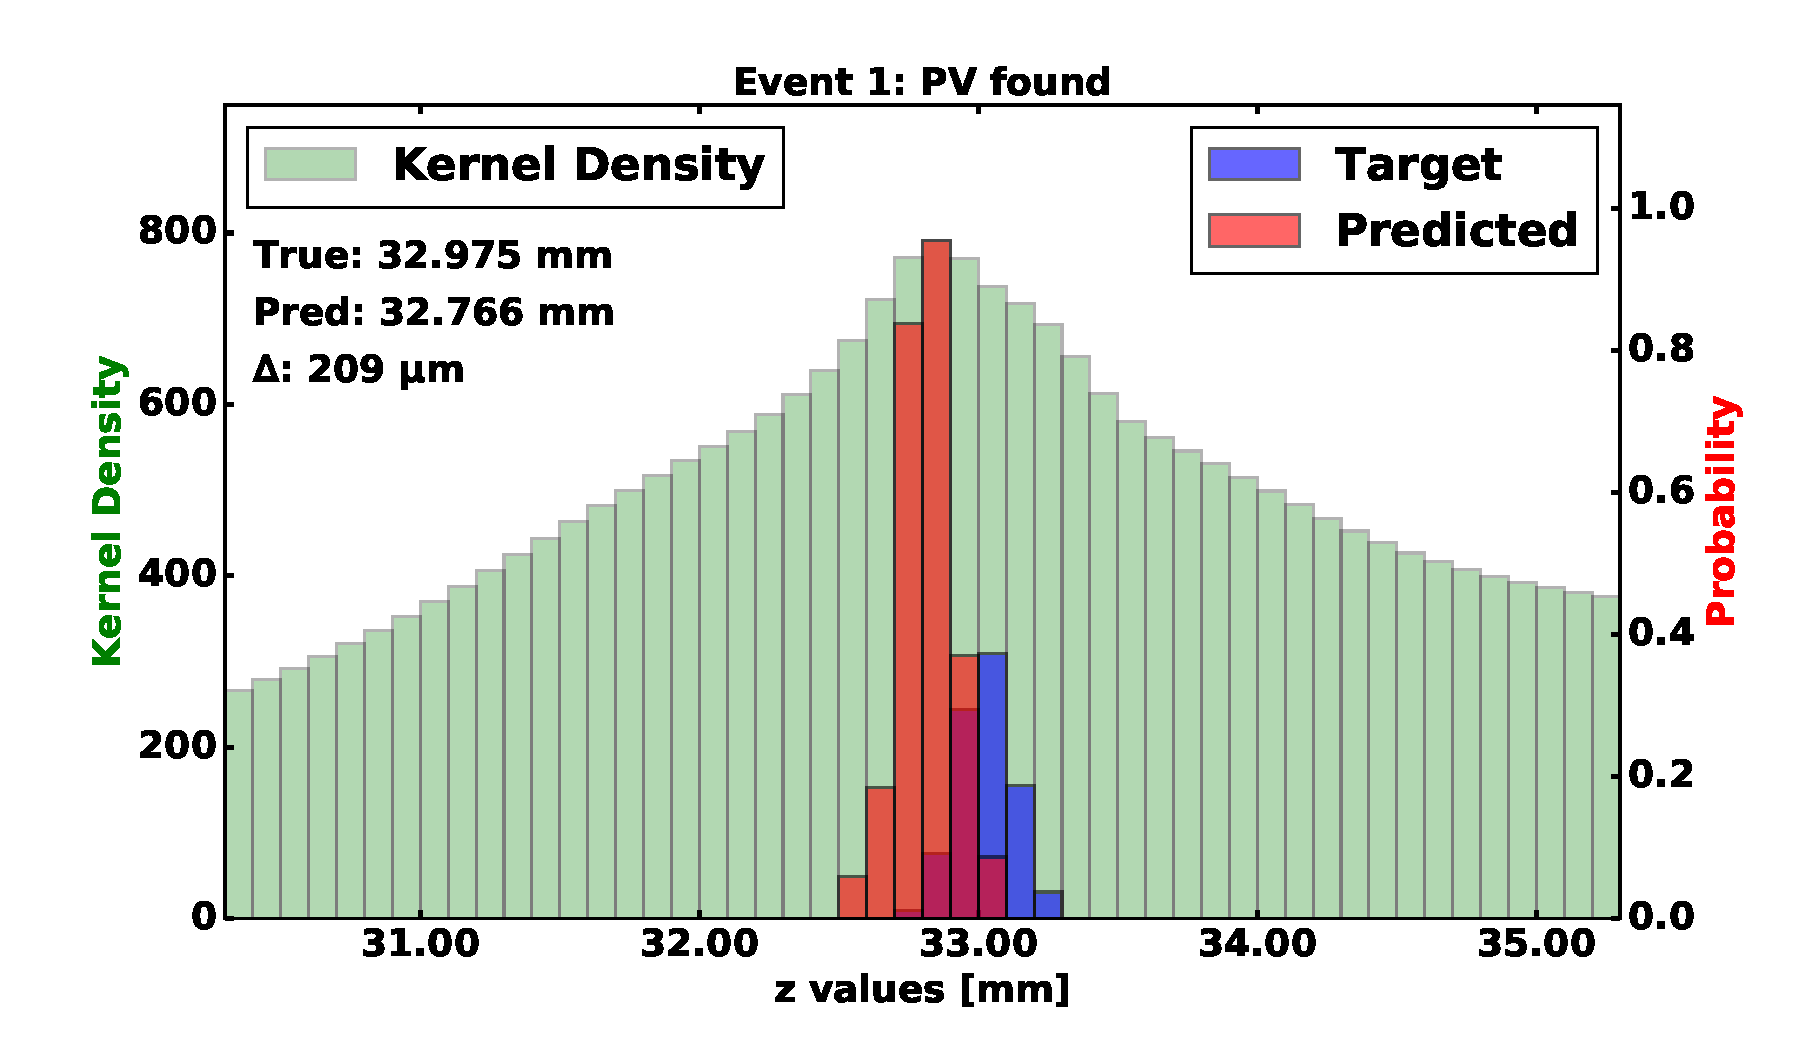
\includegraphics[width=1\textwidth,height=0.45\textwidth, trim=18 0 18 0]{images/120000_3layer_04.pdf}

            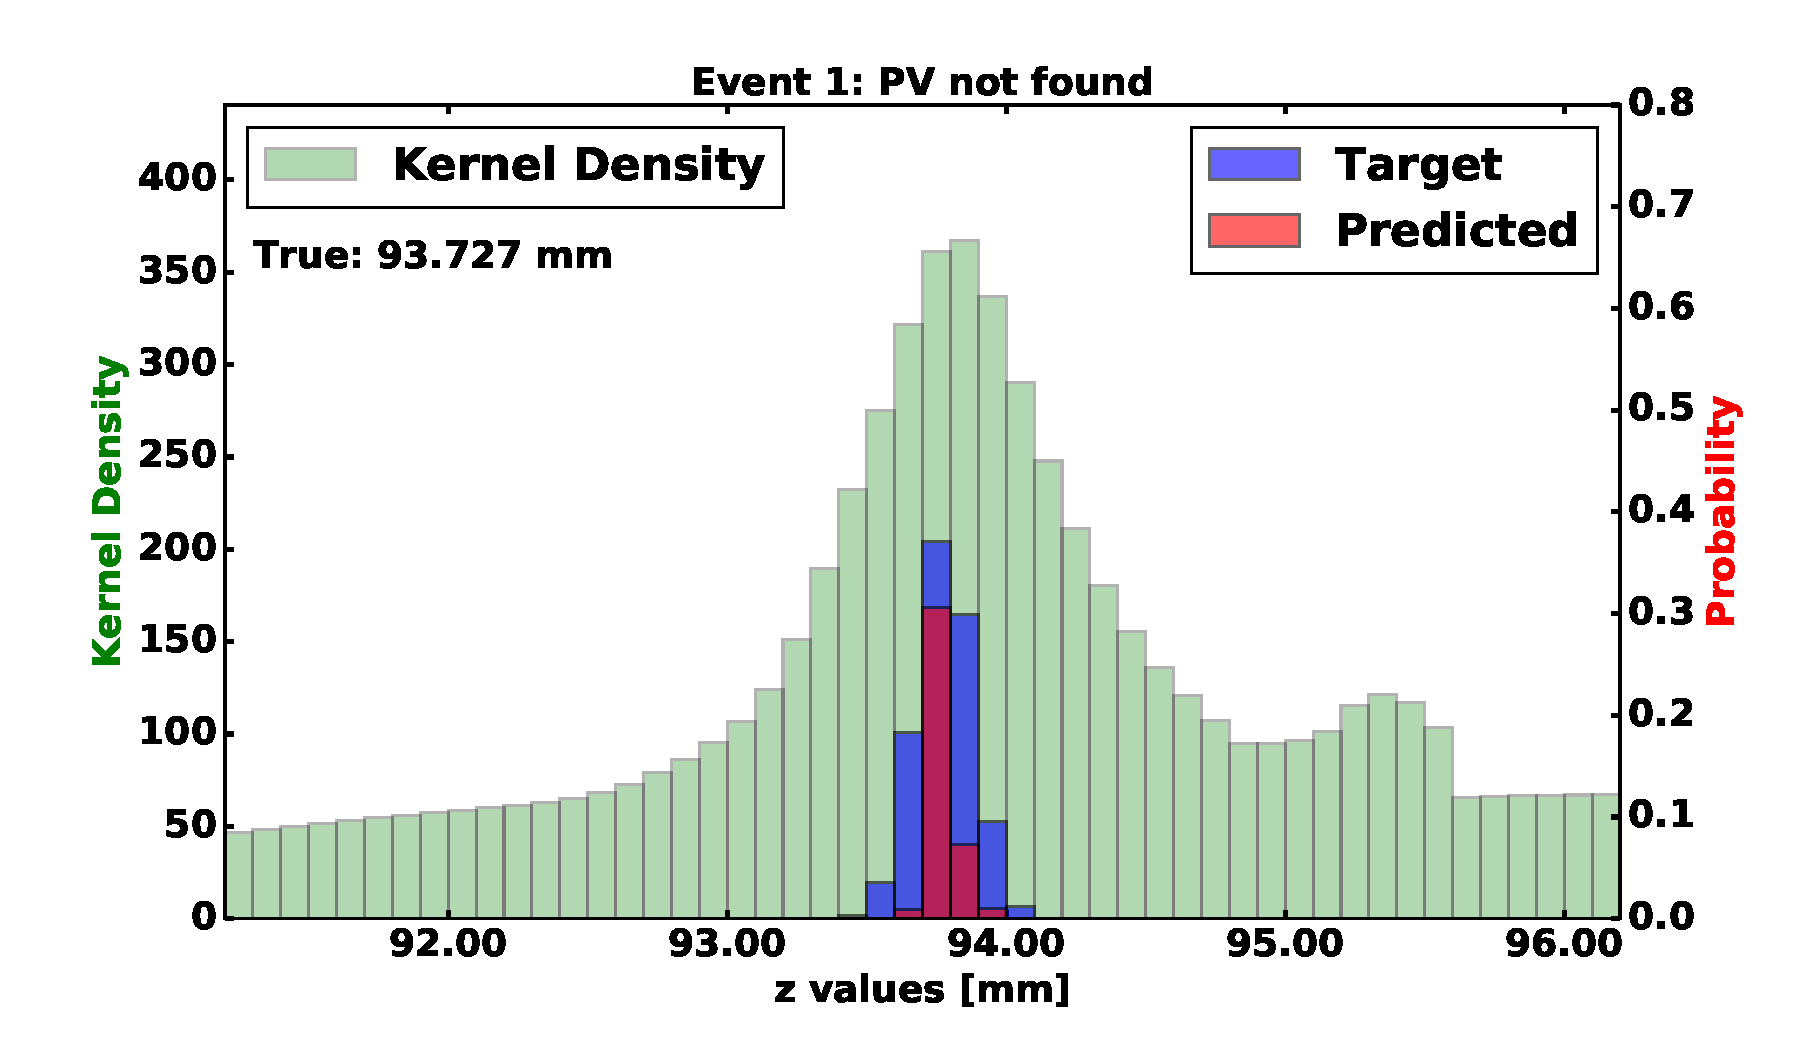
\includegraphics[width=1\textwidth, height=0.45\textwidth,trim=18 0 18 0]{images/120000_3layer_05.pdf}

        \end{center}
    \column{.5\textwidth}
        \begin{center}
           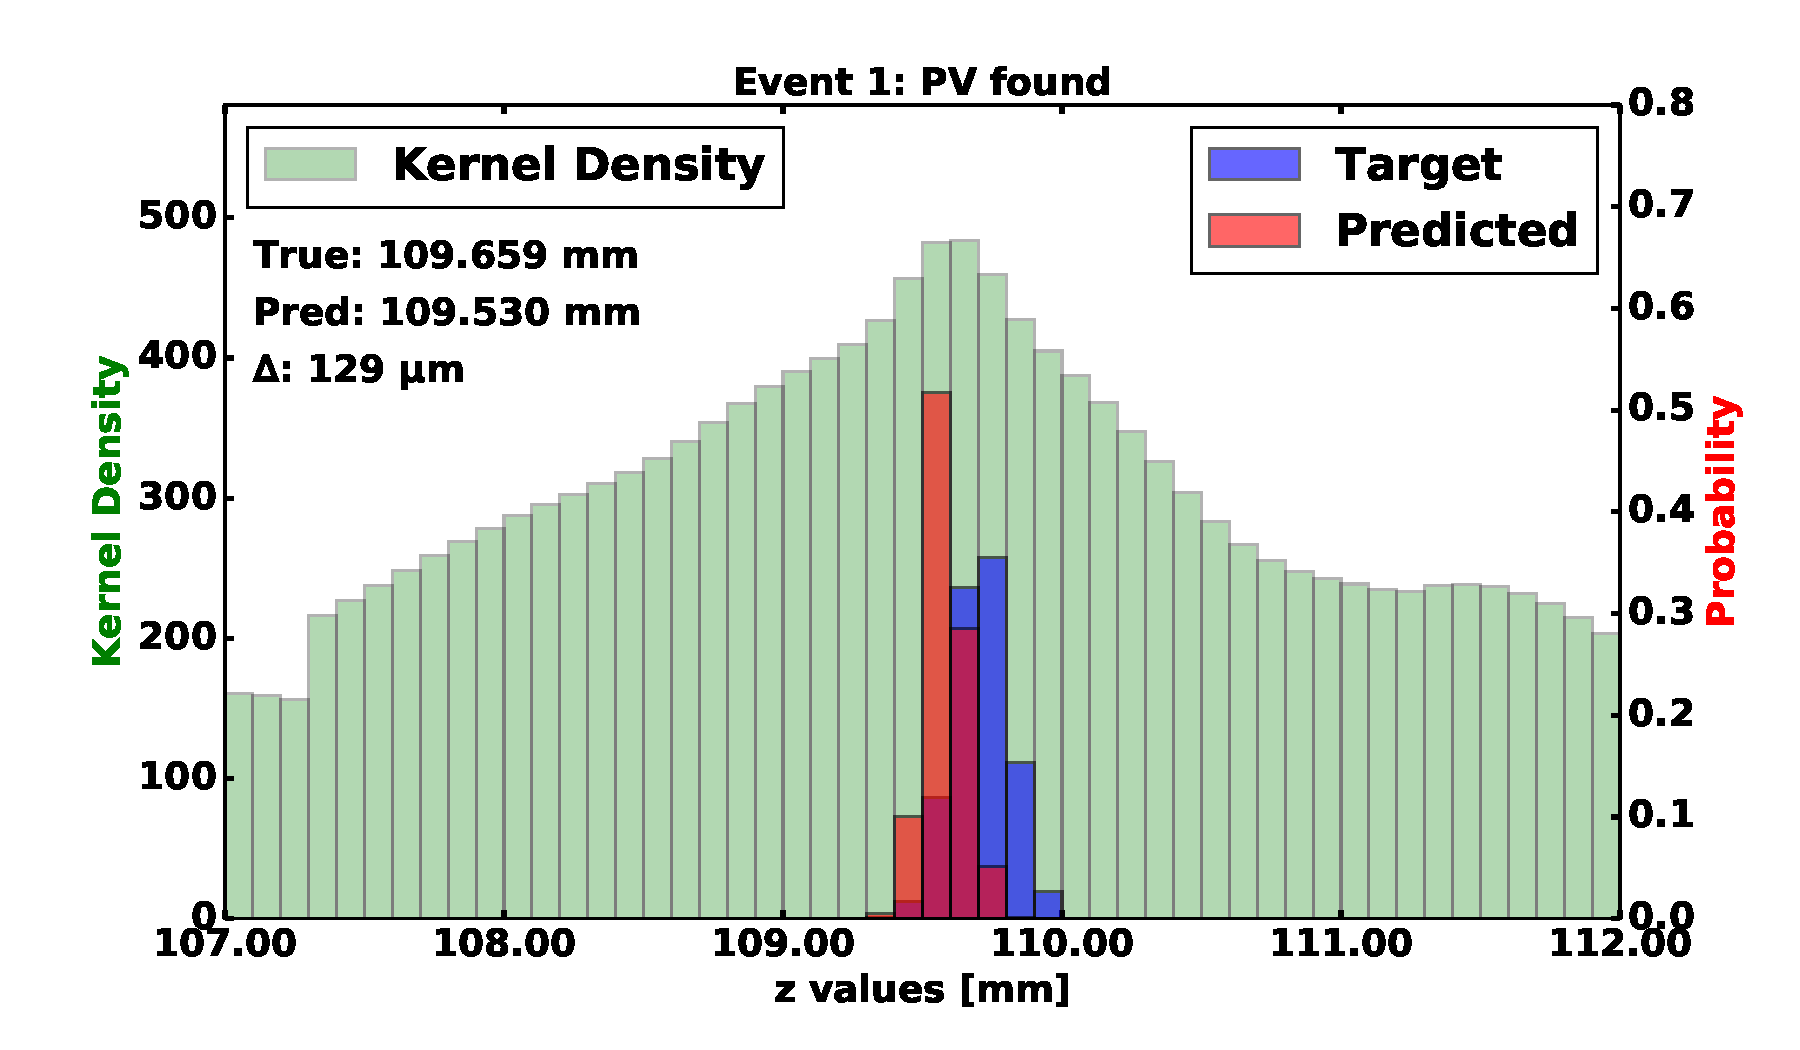
\includegraphics[width=1\textwidth, height=0.45\textwidth, trim=18 0 18 0]{images/120000_3layer_06.pdf}

           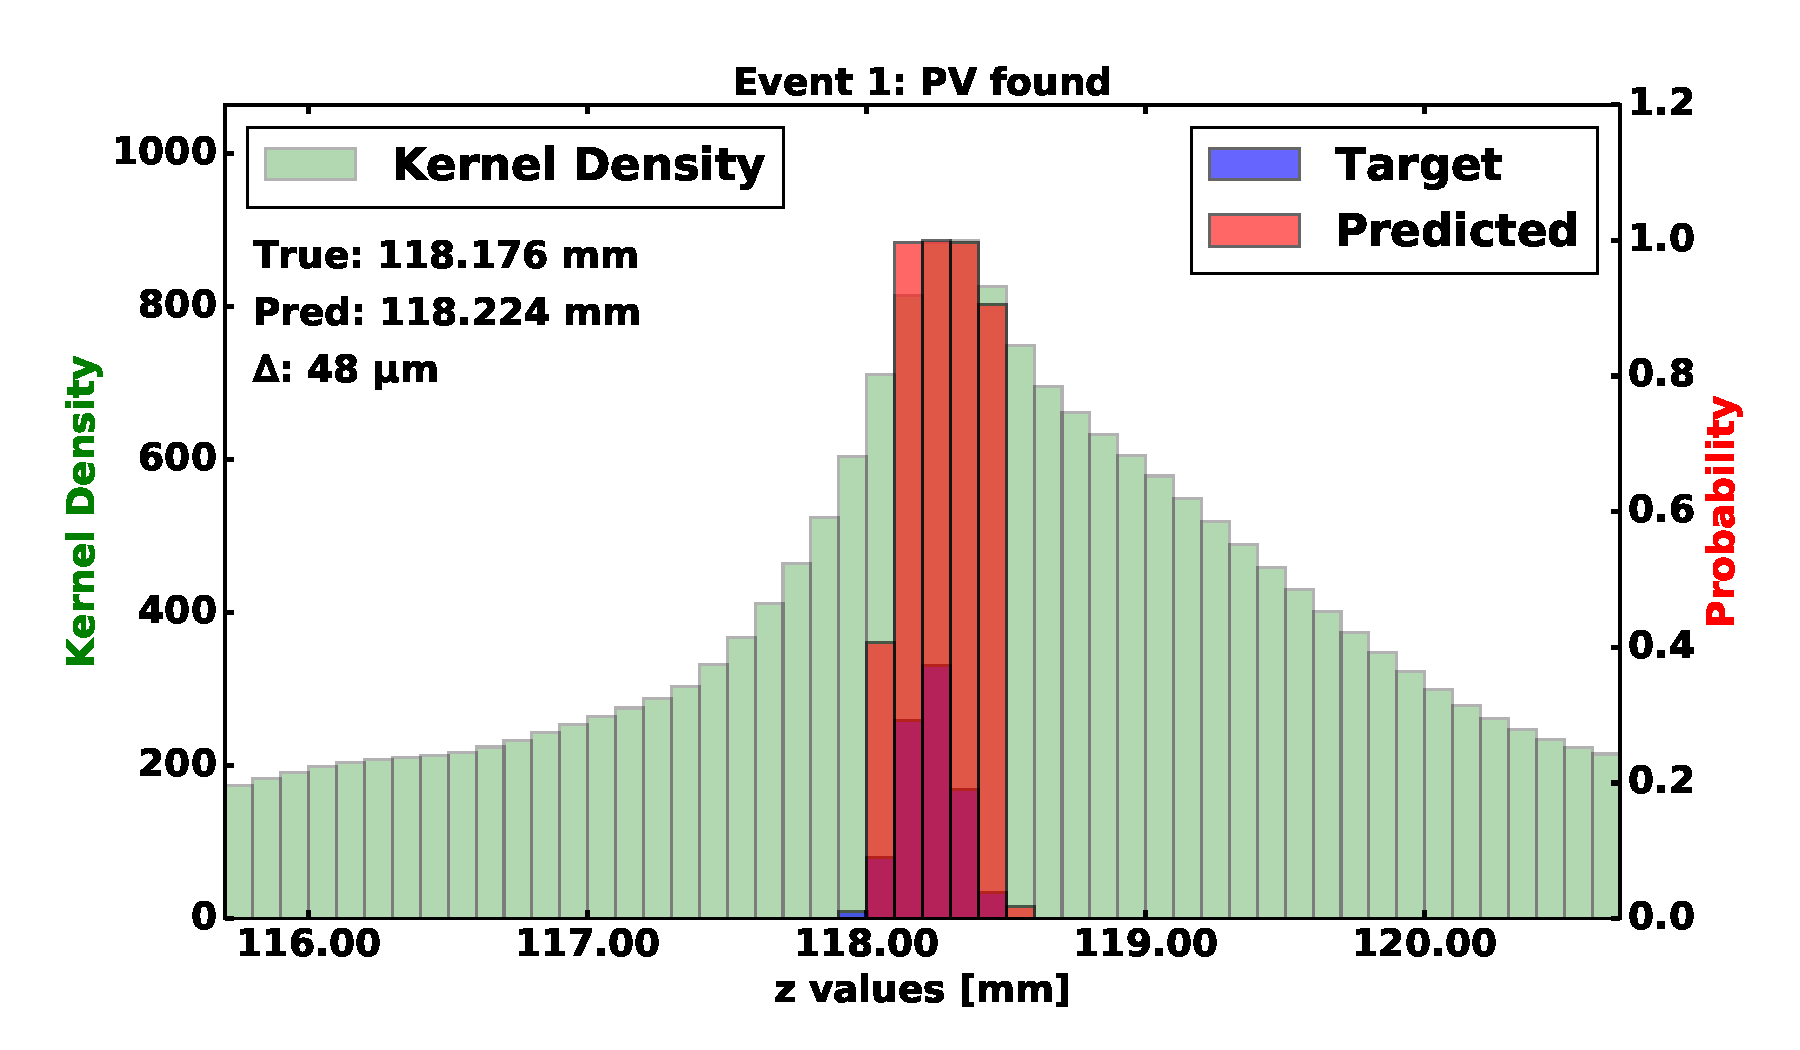
\includegraphics[width=1\textwidth, height=0.45\textwidth, trim=18 0 18 0]{images/120000_3layer_07.pdf}
       \end{center}
  \end{columns}
\end{frame}

\begin{frame}{Compare predictions with targets (3 convolutional layers)}
  \begin{columns}[c]
    \column{.5\textwidth}
        \begin{center}
            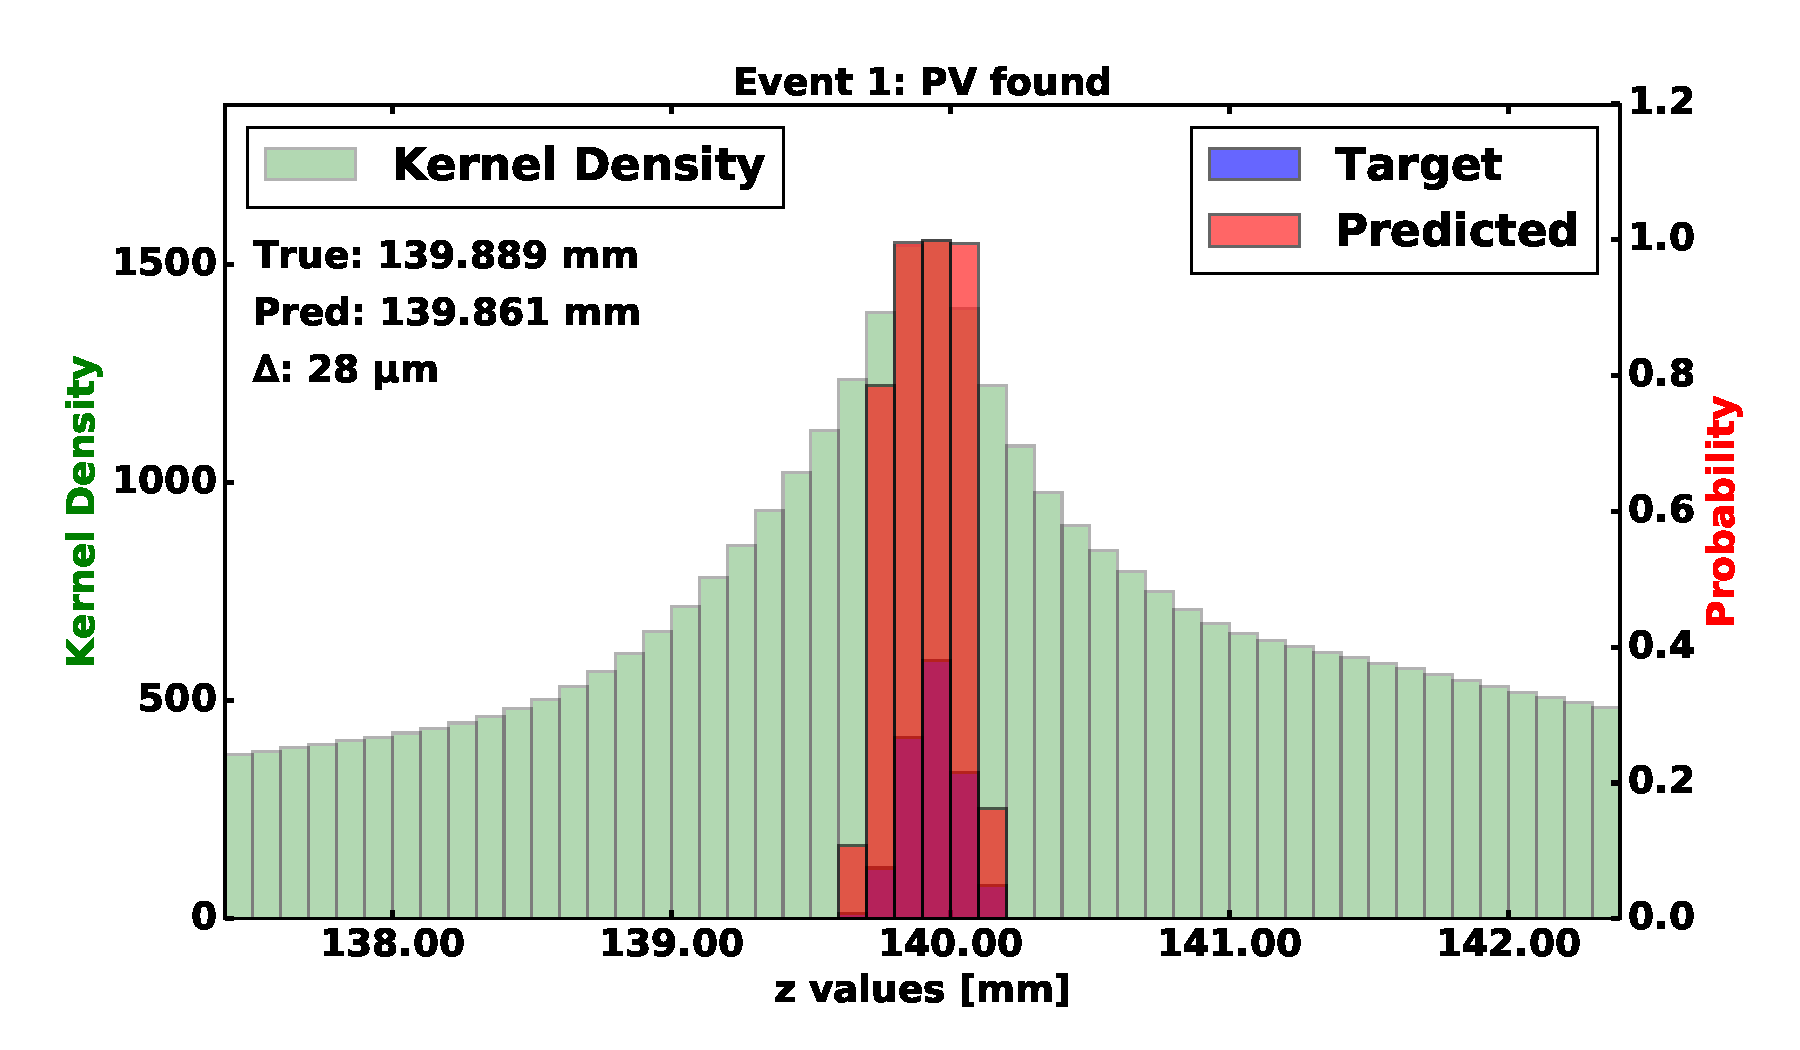
\includegraphics[width=1\textwidth,height=0.45\textwidth, trim=18 0 18 0]{images/120000_3layer_08.pdf}

            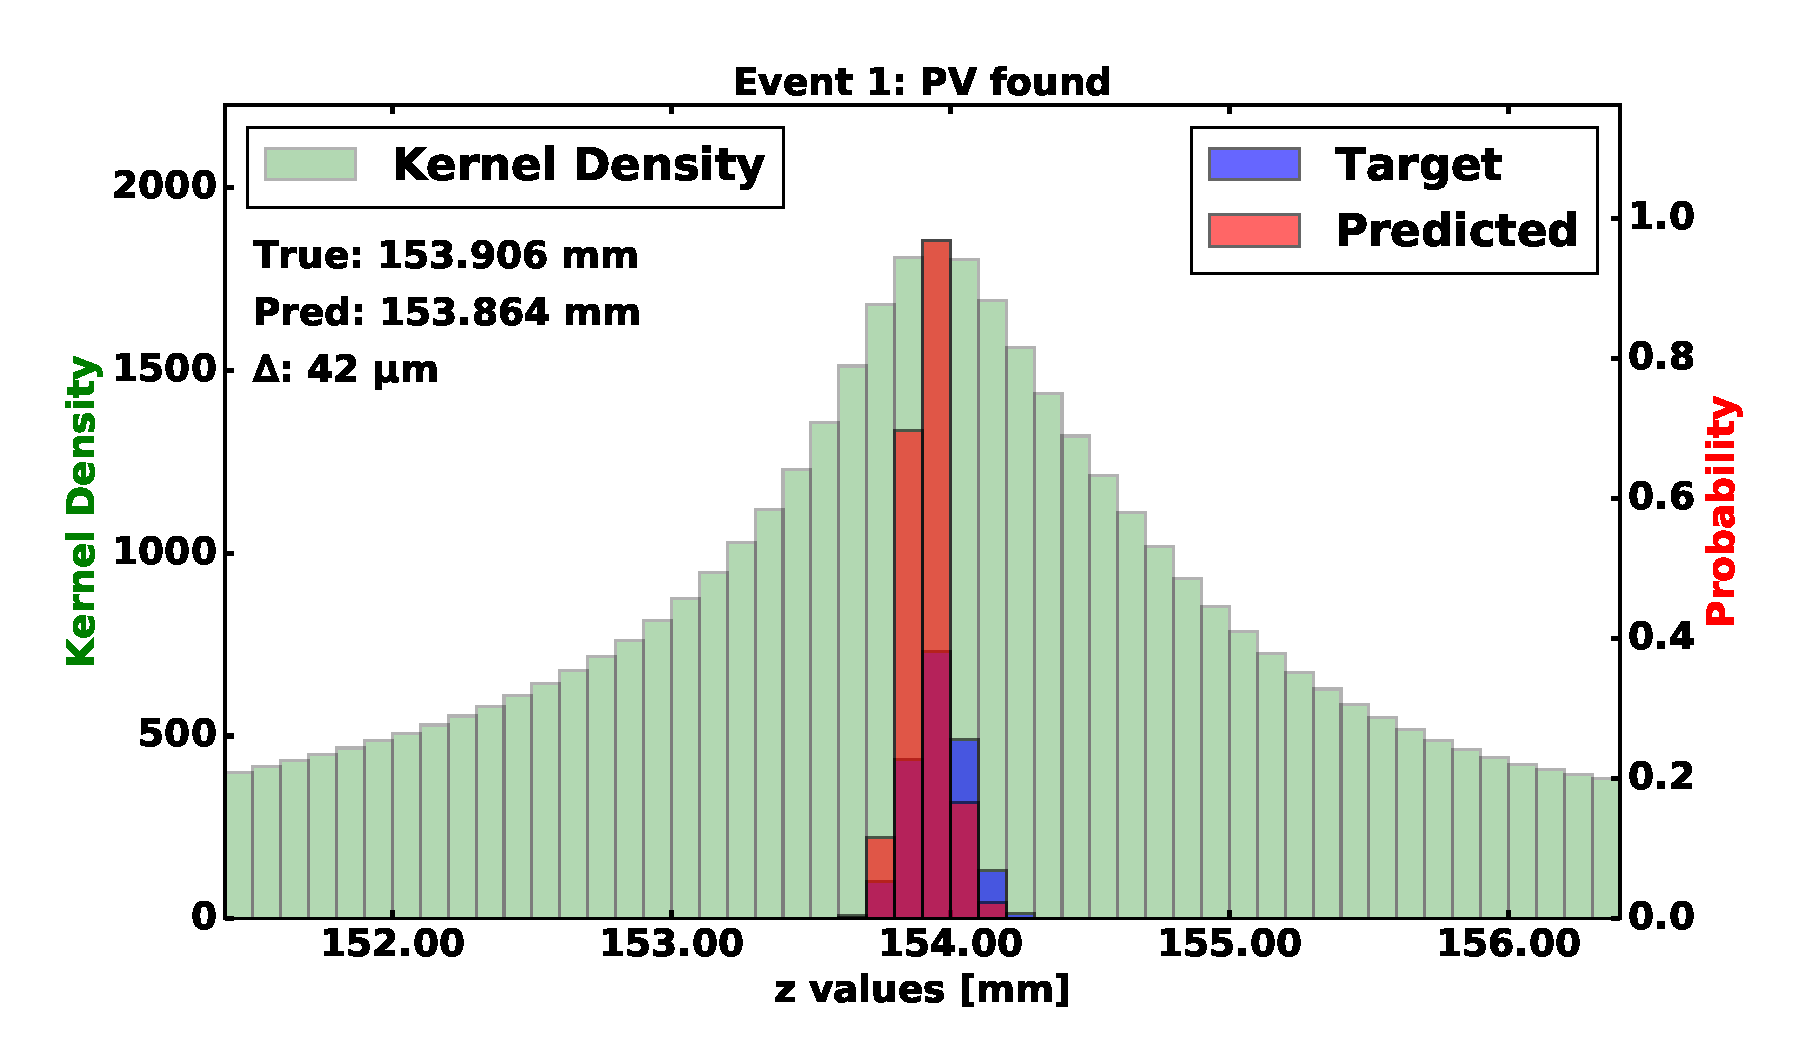
\includegraphics[width=1\textwidth, height=0.45\textwidth,trim=18 0 18 0]{images/120000_3layer_09.pdf}

        \end{center}
    \column{.5\textwidth}
        \begin{center}
           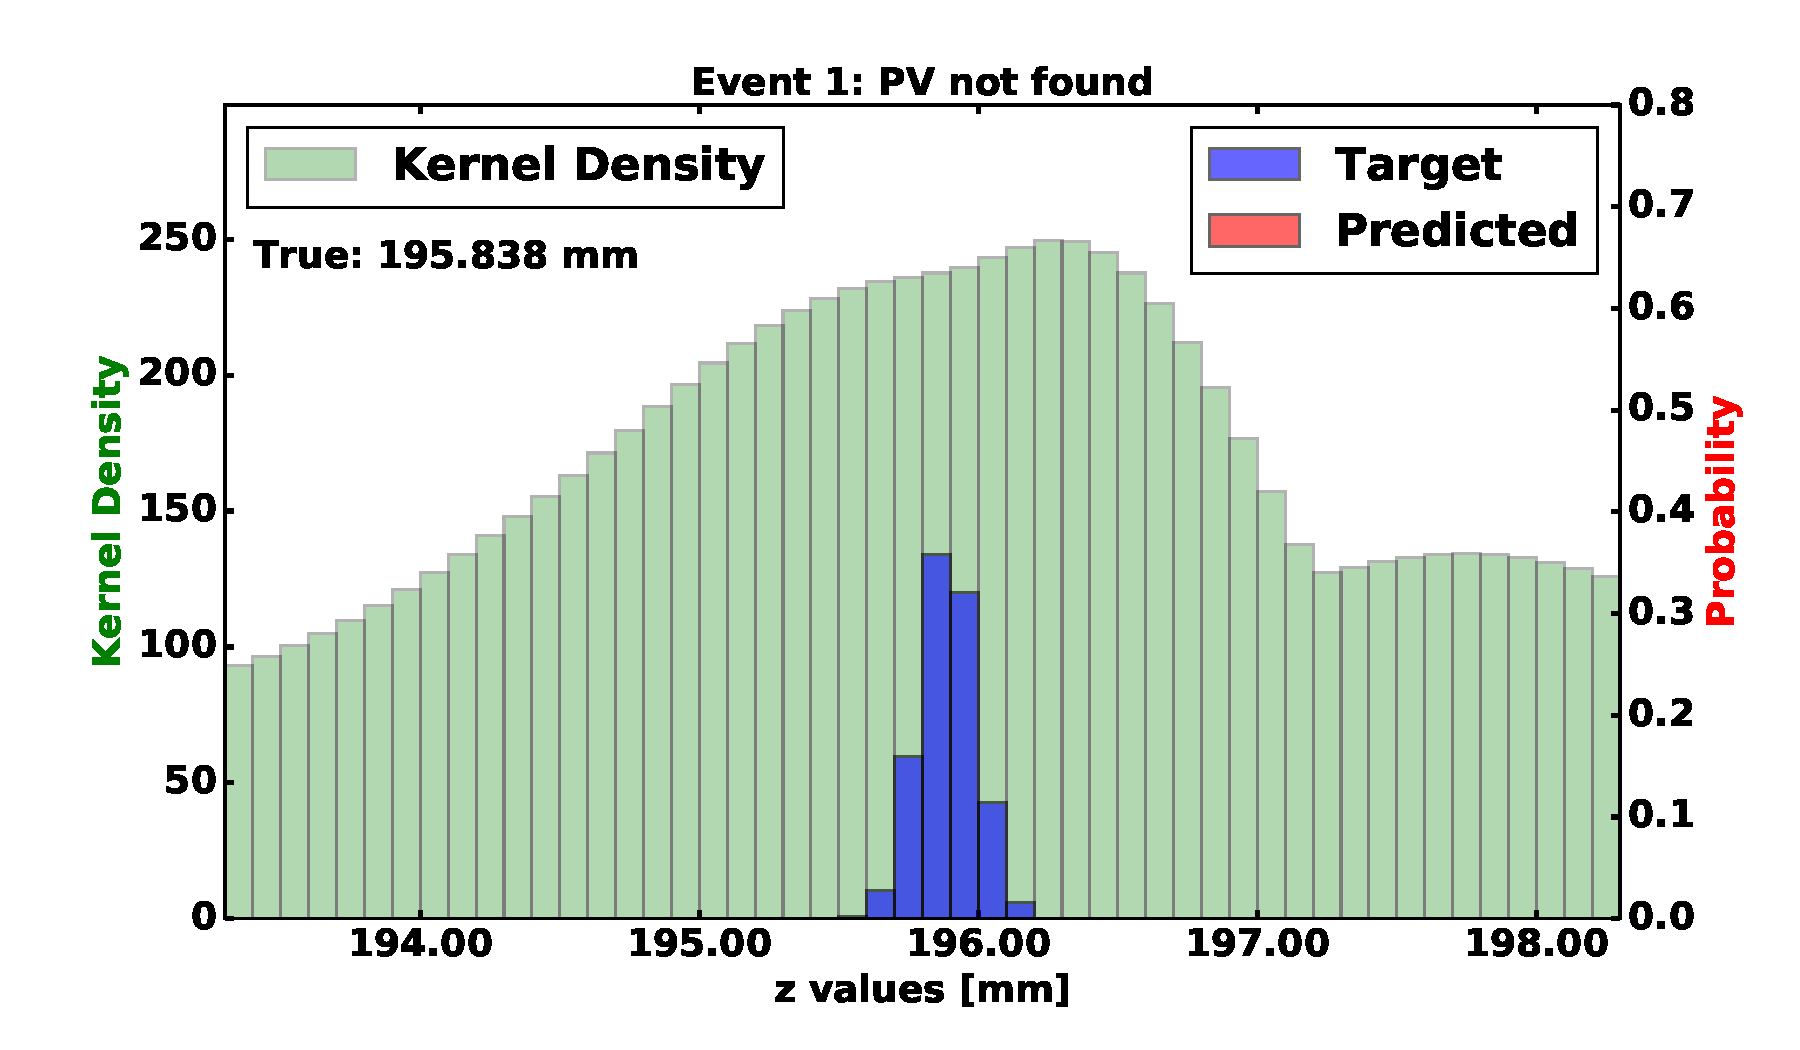
\includegraphics[width=1\textwidth, height=0.45\textwidth, trim=18 0 18 0]{images/120000_3layer_10.pdf}

           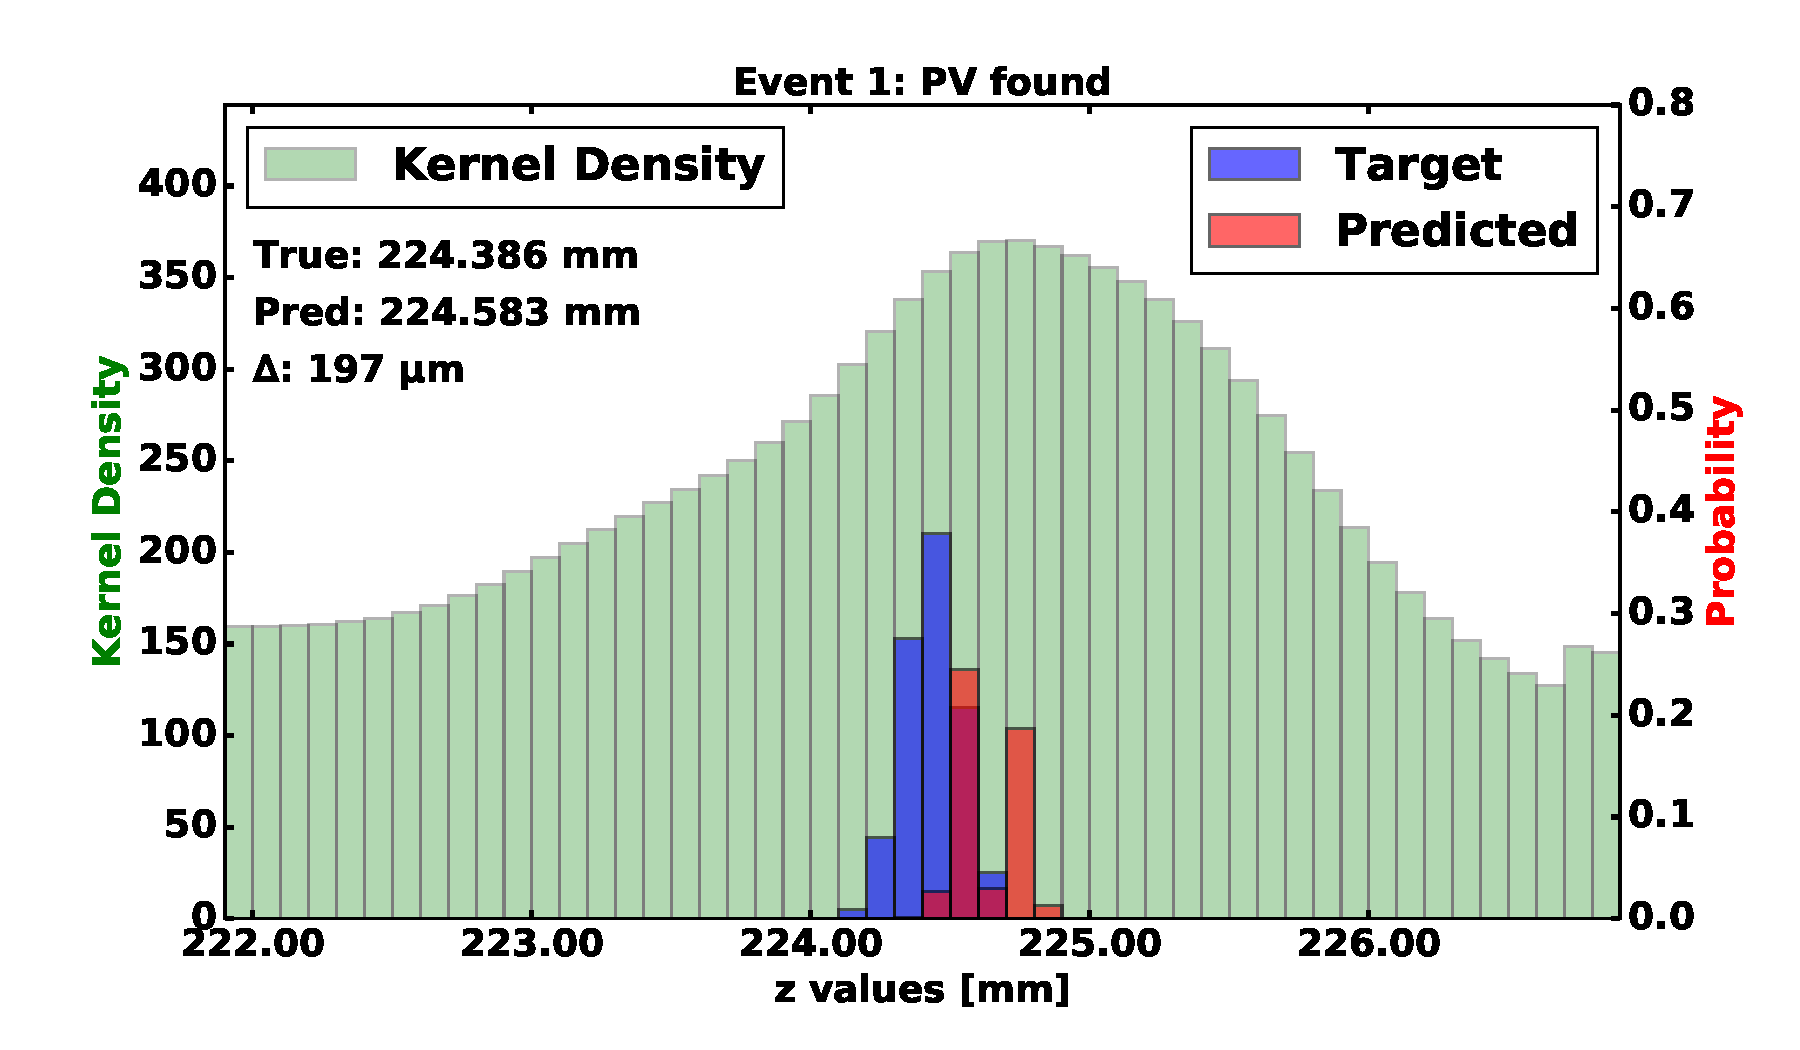
\includegraphics[width=1\textwidth, height=0.45\textwidth, trim=18 0 18 0]{images/120000_3layer_11.pdf}
       \end{center}
  \end{columns}
\end{frame}

\subsection{More predictions with targets}

\begin{frame}{More predictions with targets (3 CVN layers)}
  \begin{columns}[c]
    \column{.5\textwidth}
        \begin{center}
            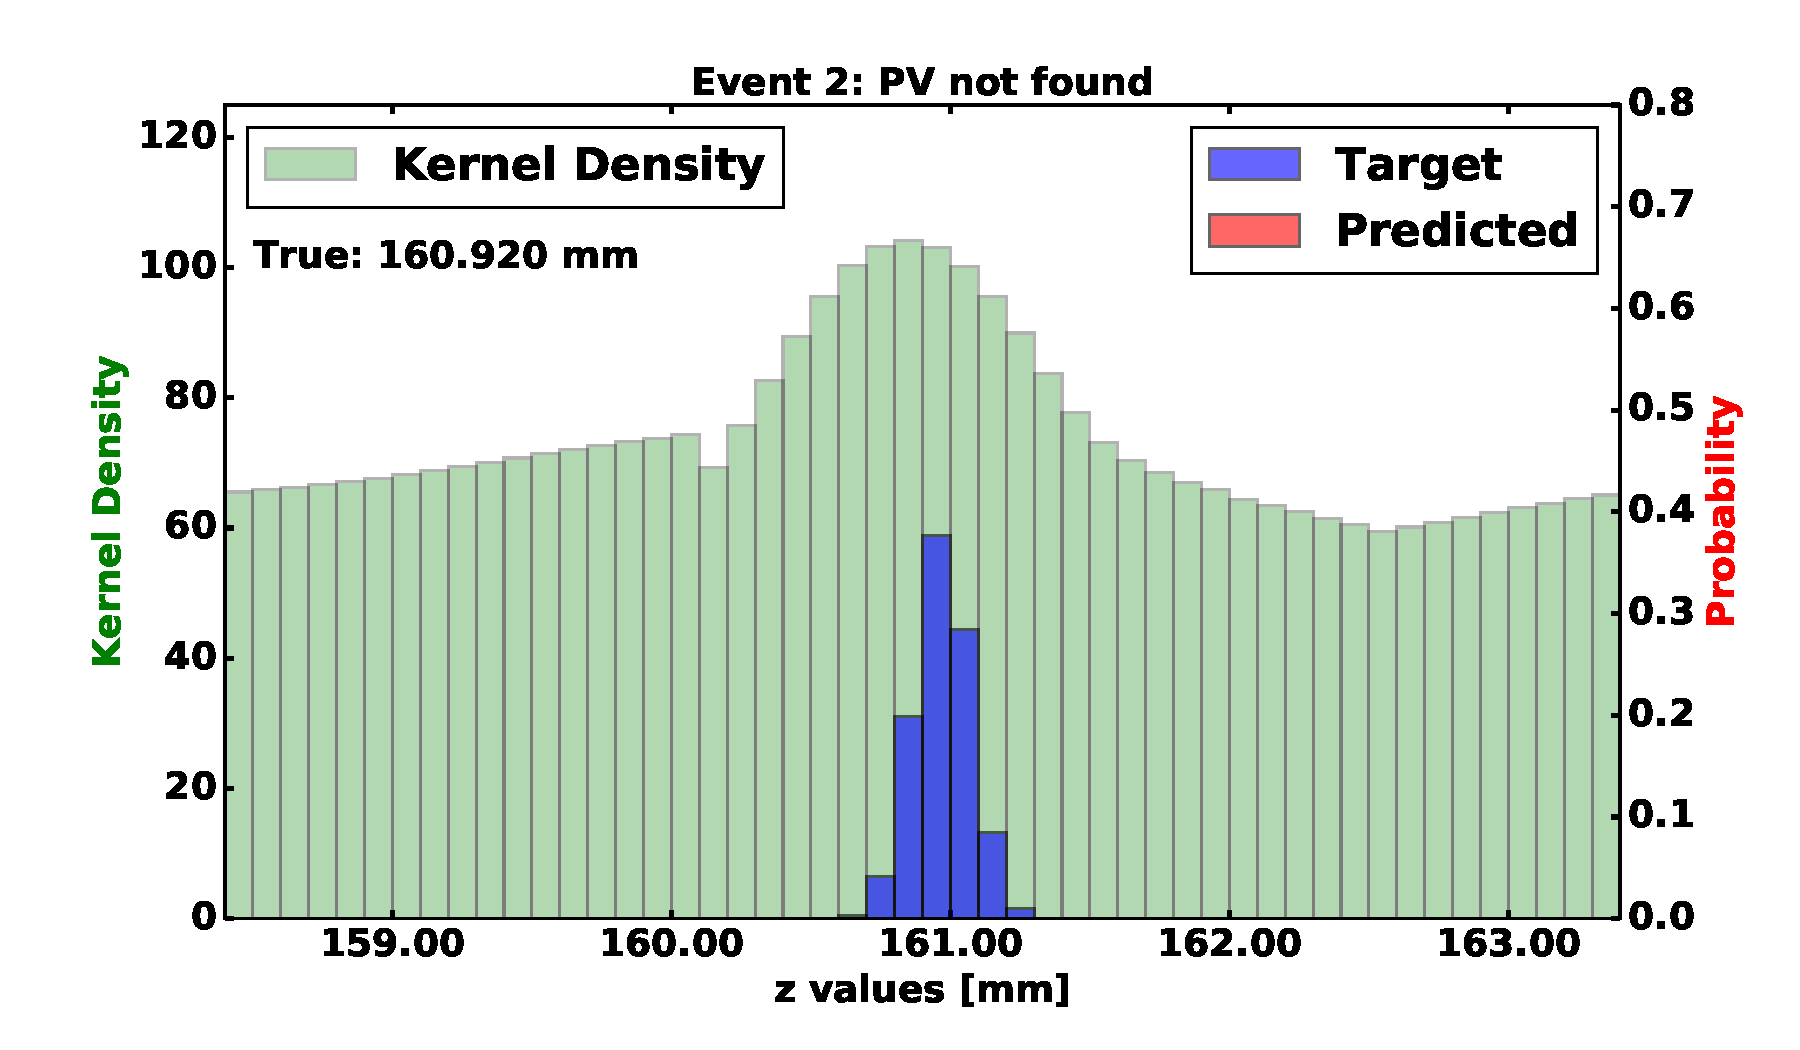
\includegraphics[width=1\textwidth,height=0.45\textwidth, trim=18 0 18 0]{images/120000_3layer_16.pdf}

            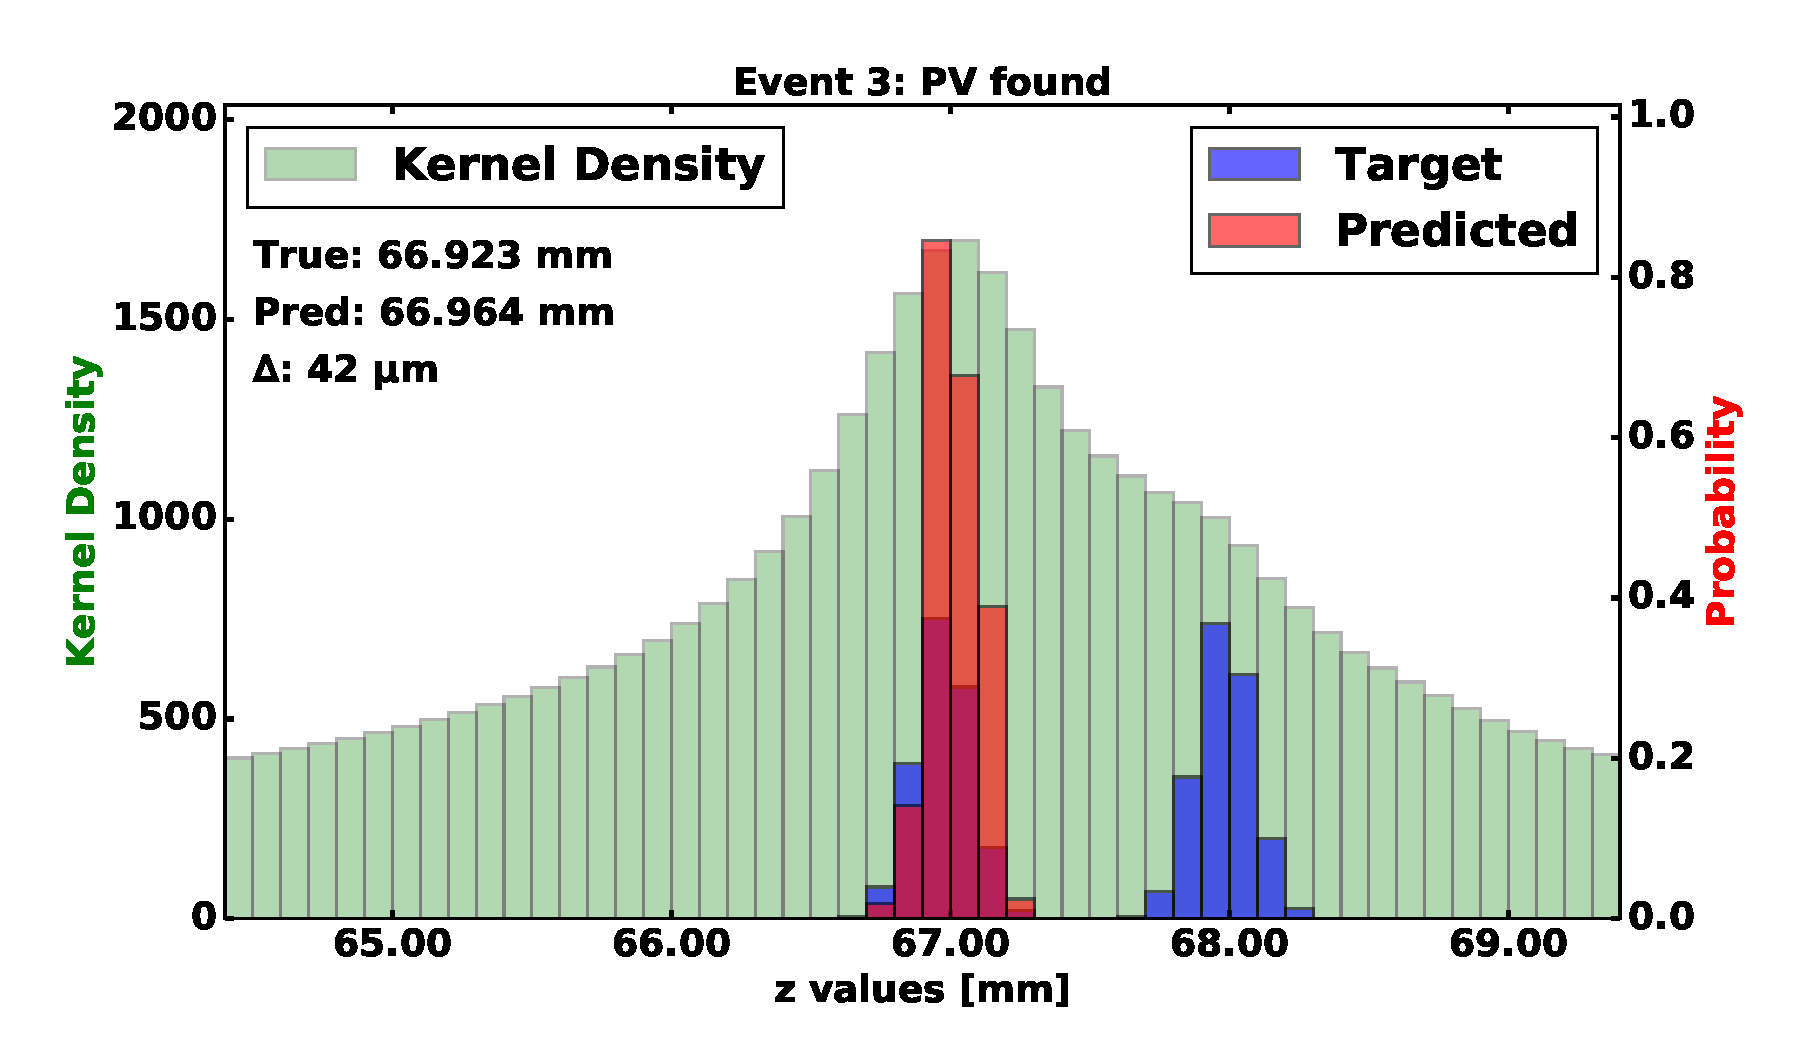
\includegraphics[width=1\textwidth, height=0.45\textwidth,trim=18 0 18 0]{images/120000_3layer_17.pdf}

        \end{center}
    \column{.5\textwidth}
        \begin{center}
           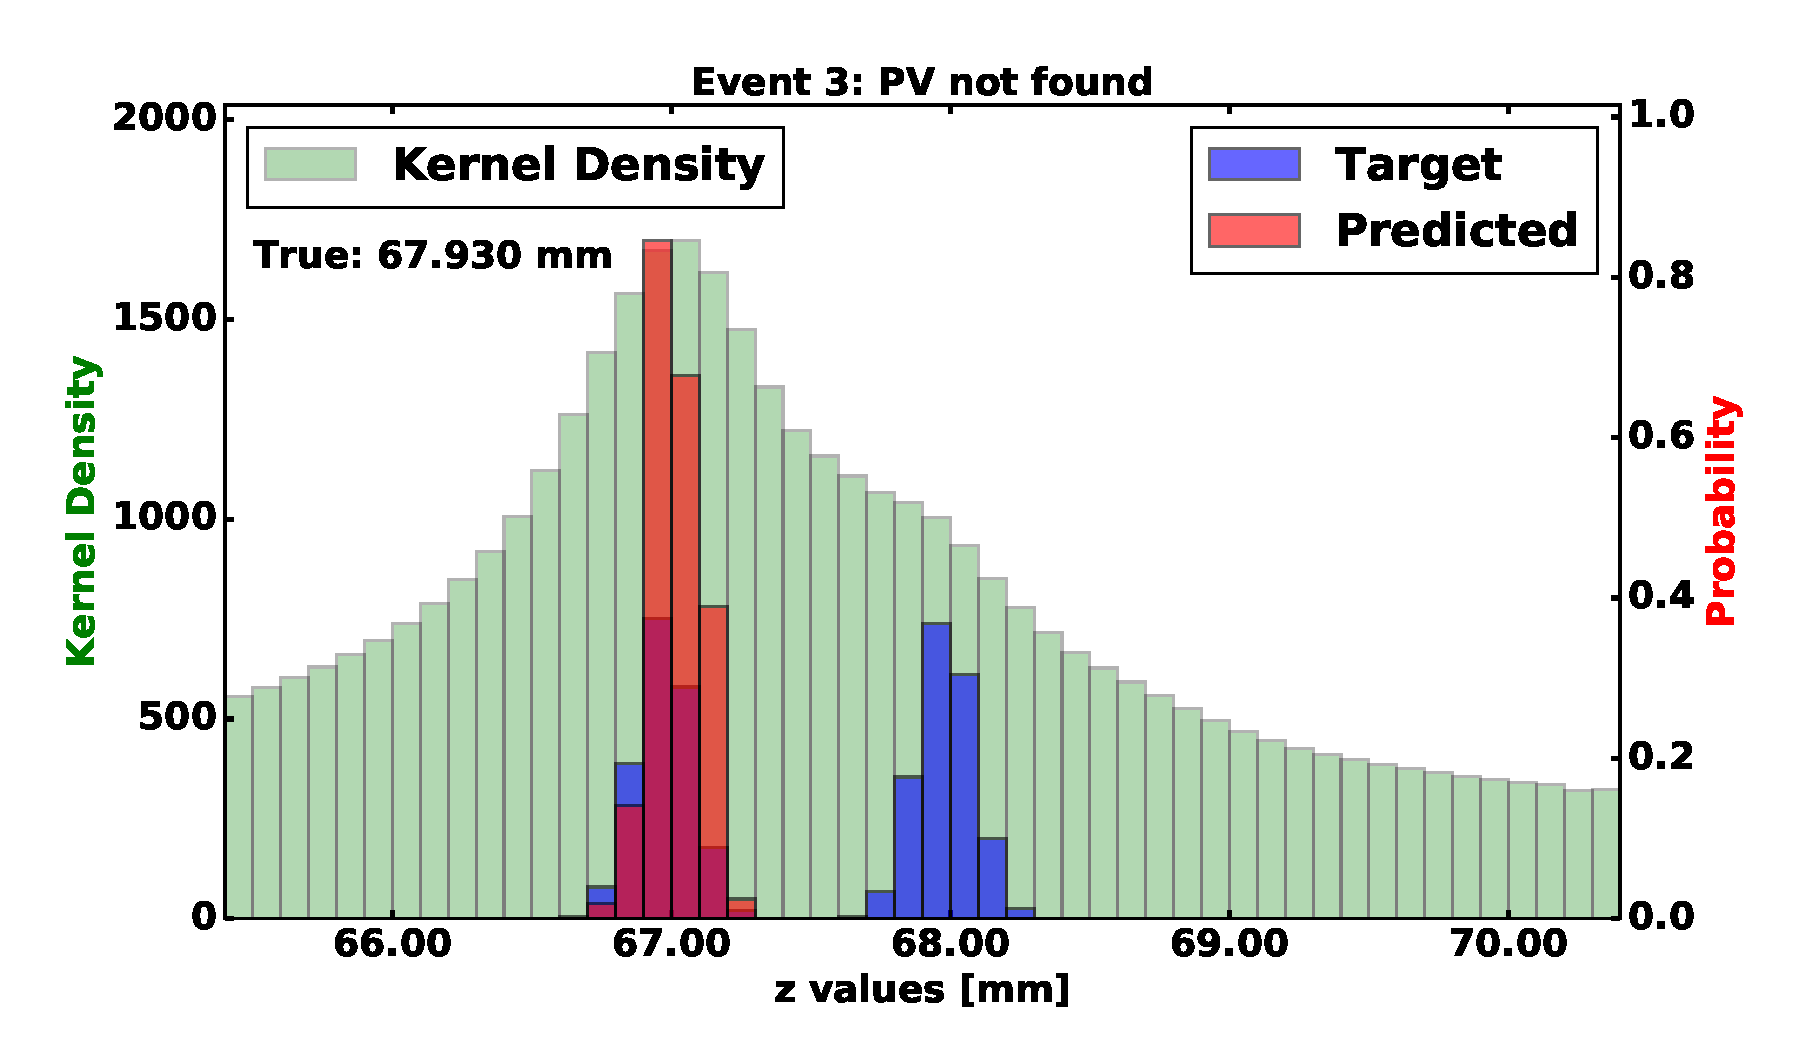
\includegraphics[width=1\textwidth, height=0.45\textwidth, trim=18 0 18 0]{images/120000_3layer_18.pdf}

           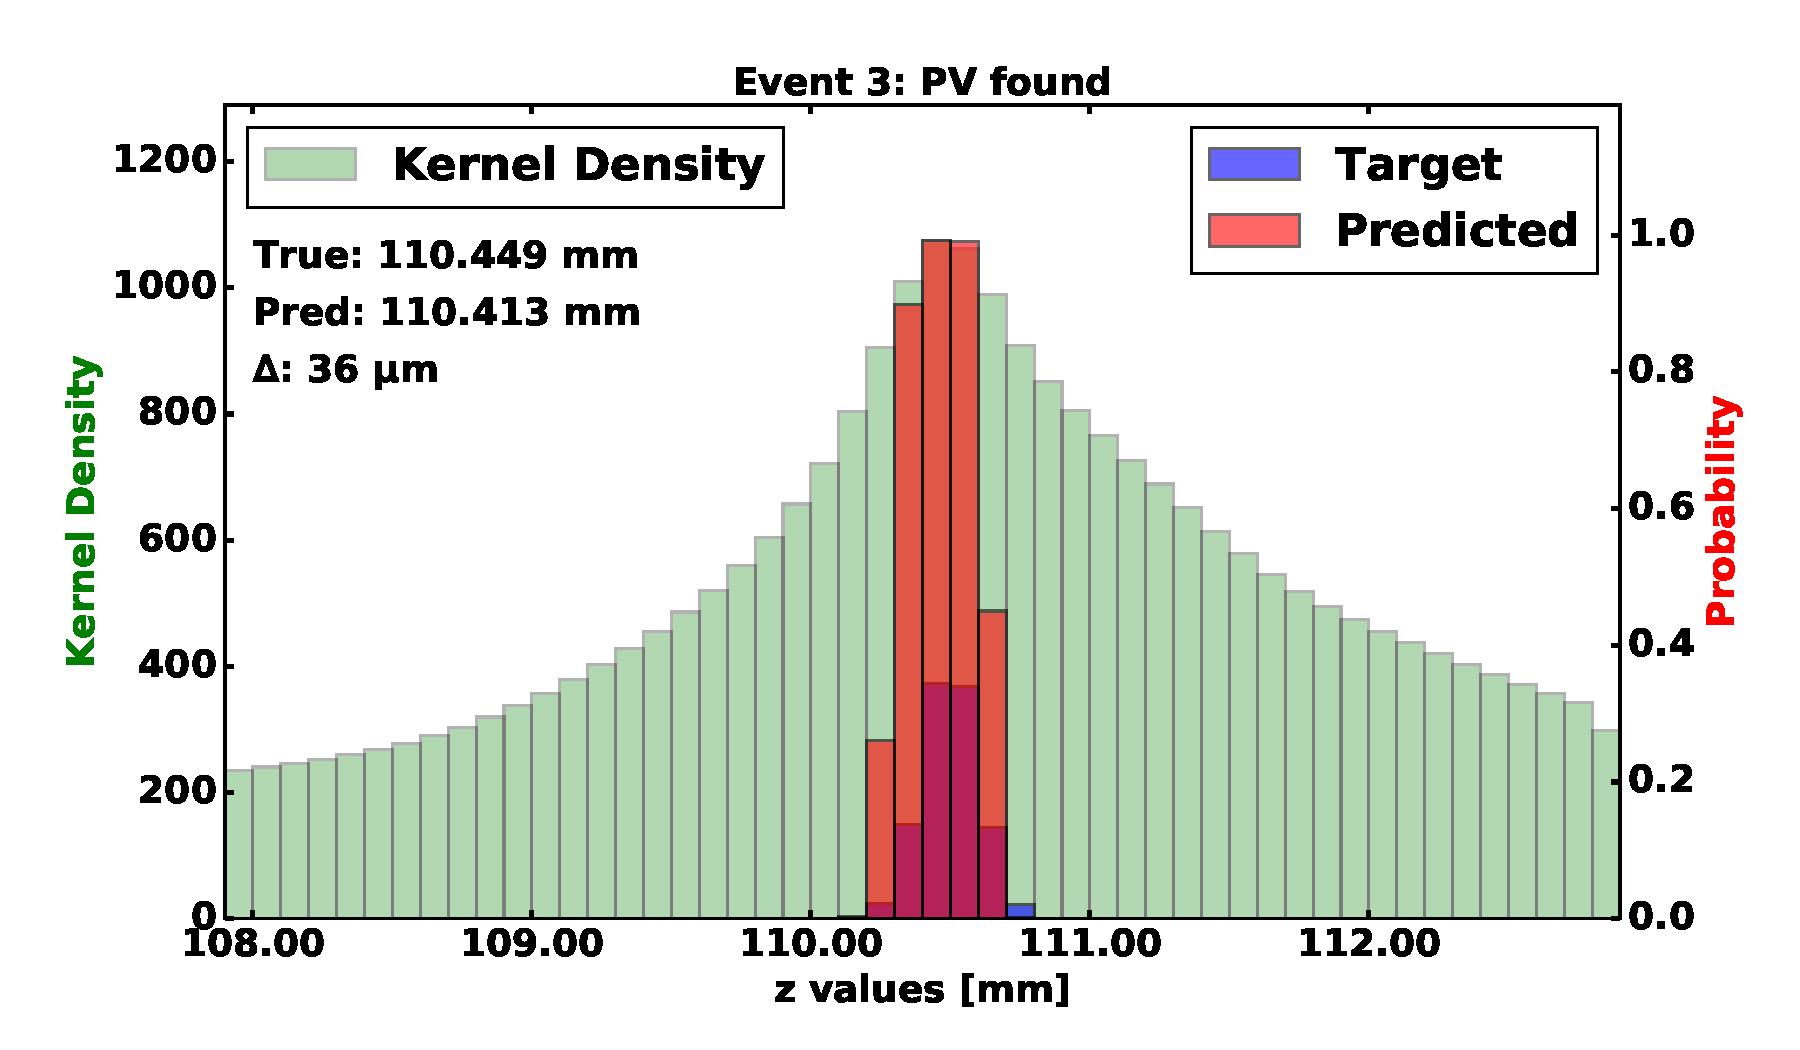
\includegraphics[width=1\textwidth, height=0.45\textwidth, trim=18 0 18 0]{images/120000_3layer_19.pdf}
       \end{center}
  \end{columns}
\end{frame}

\begin{frame}{More Predictions with Targets (3 CVN layers)}
  \begin{columns}[c]
    \column{.5\textwidth}
        \begin{center}
            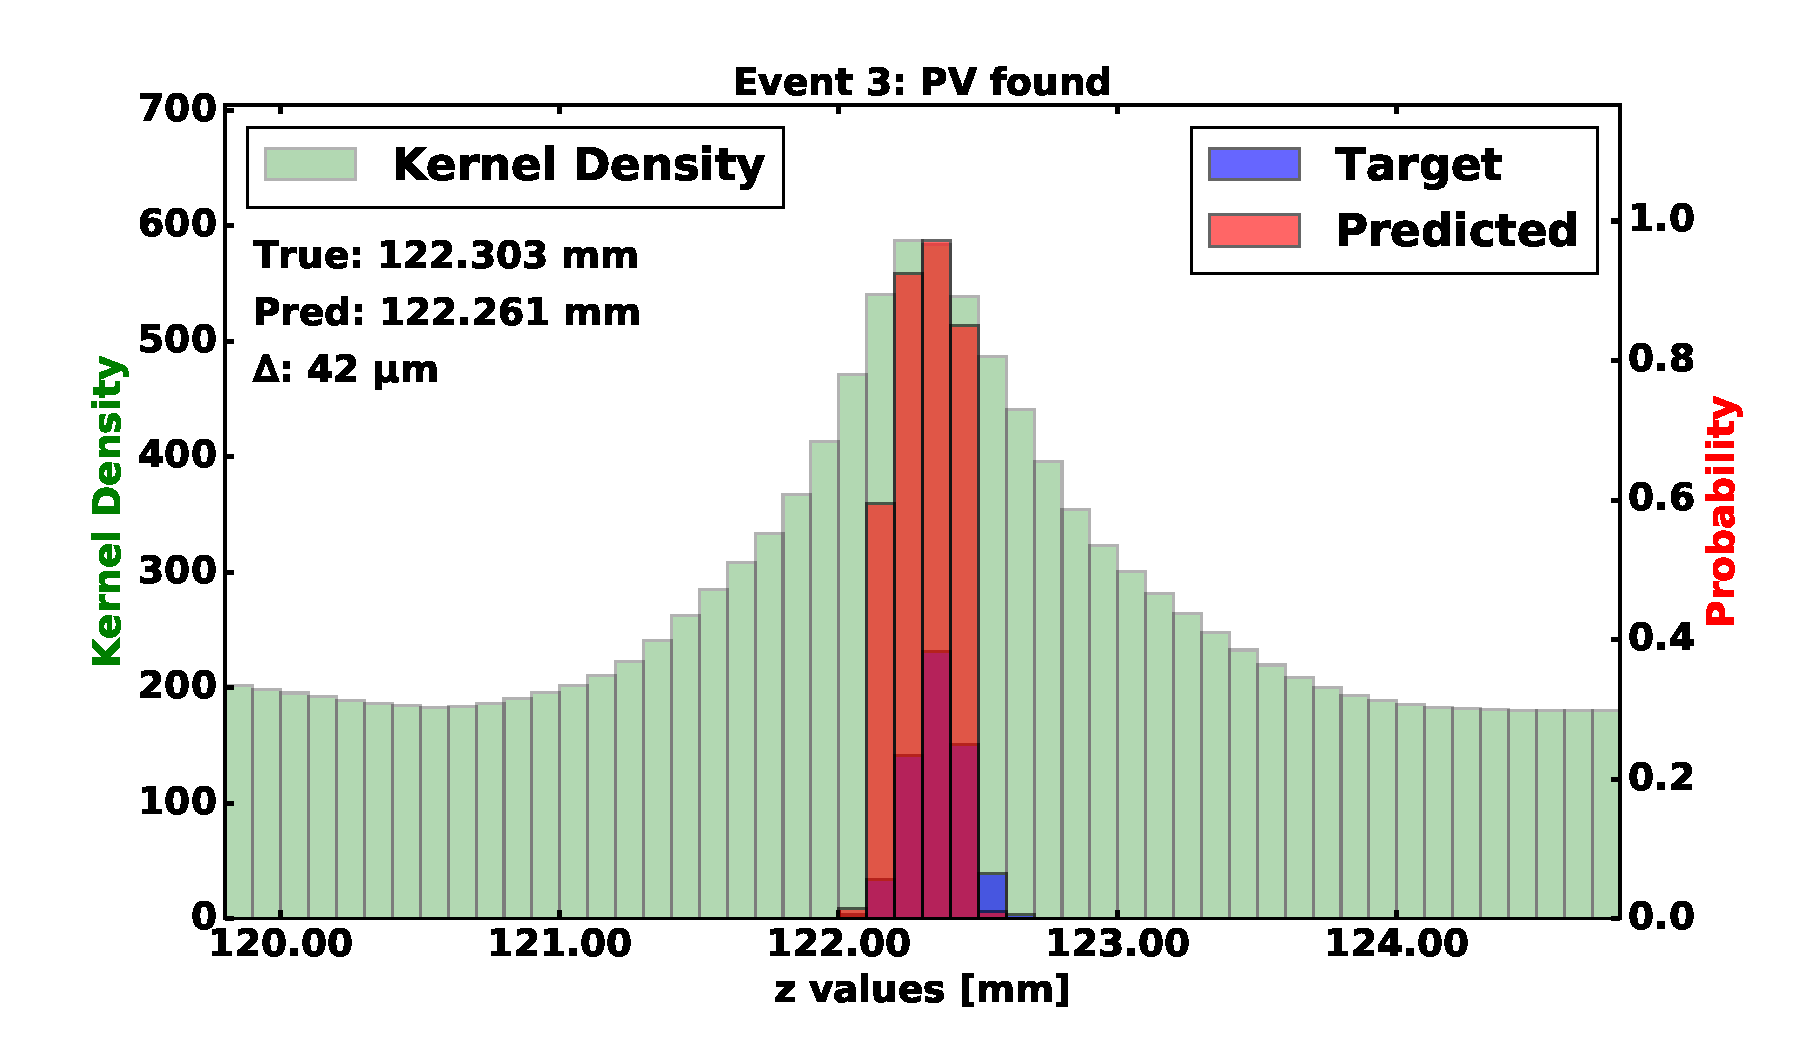
\includegraphics[width=1\textwidth,height=0.45\textwidth, trim=18 0 18 0]{images/120000_3layer_20.pdf}

            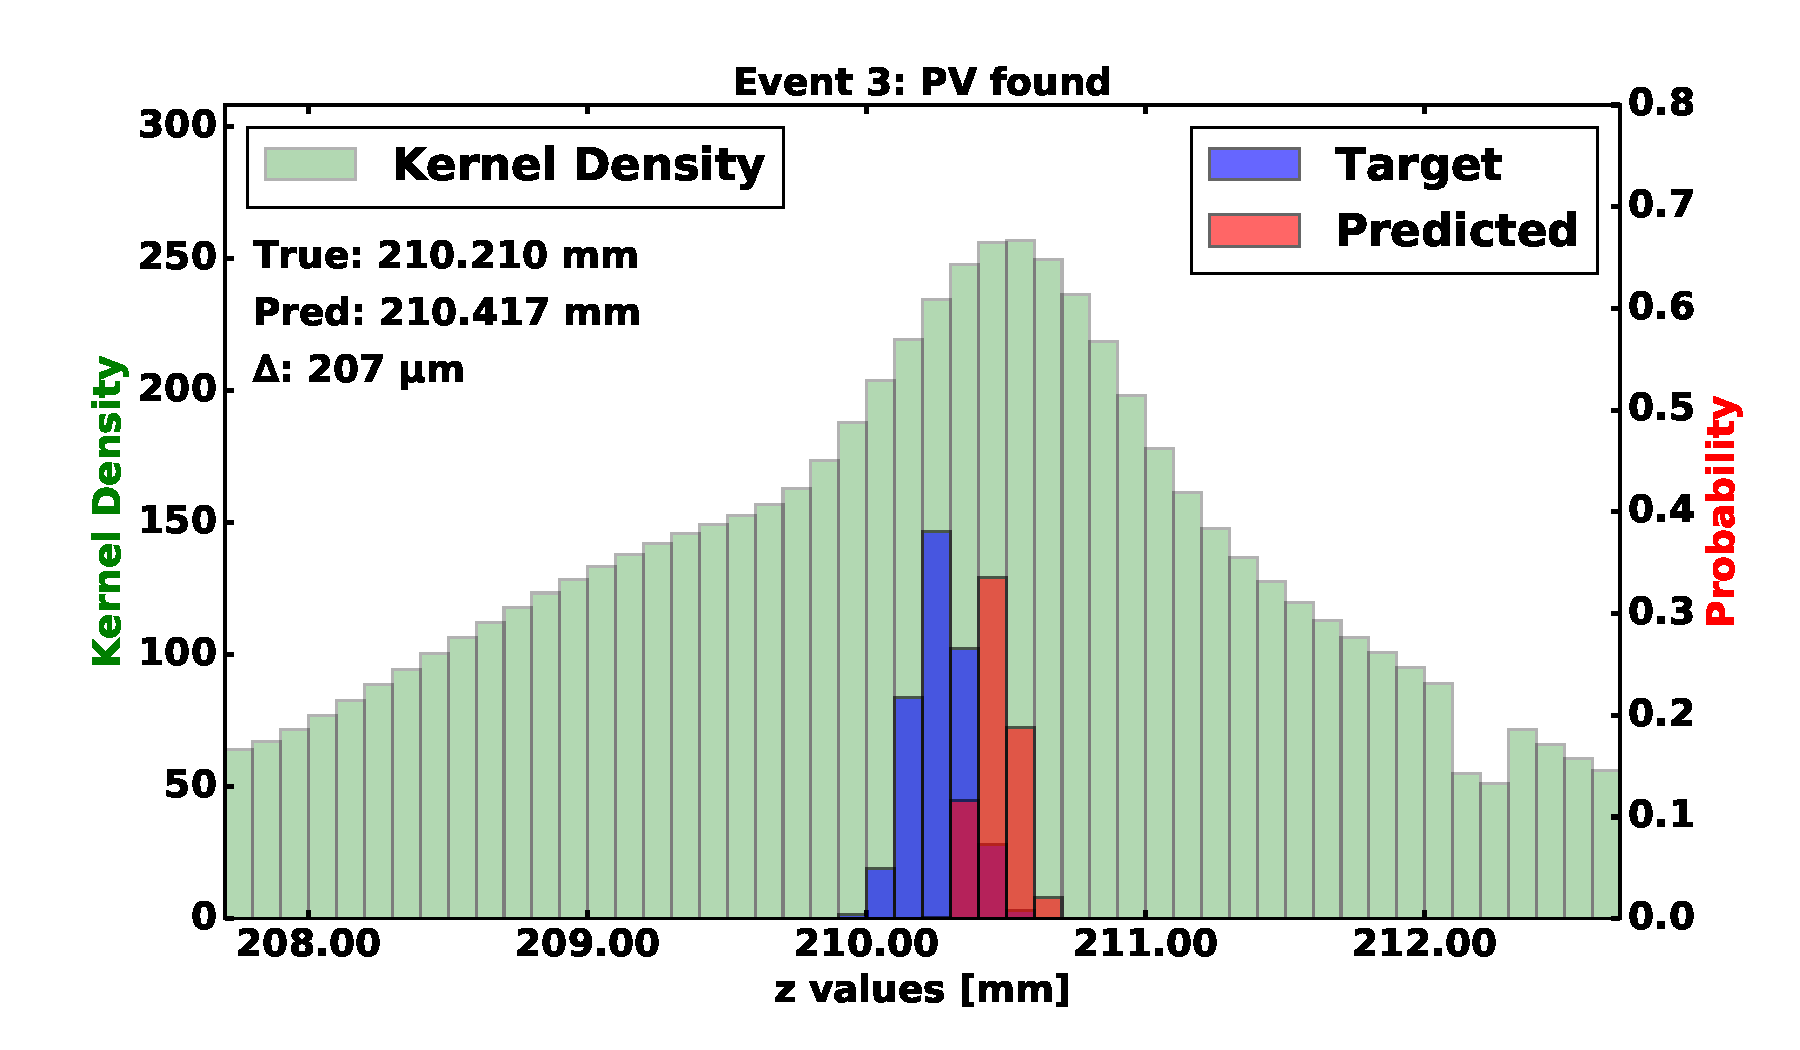
\includegraphics[width=1\textwidth, height=0.45\textwidth,trim=18 0 18 0]{images/120000_3layer_21.pdf}

        \end{center}
    \column{.5\textwidth}
        \begin{center}
           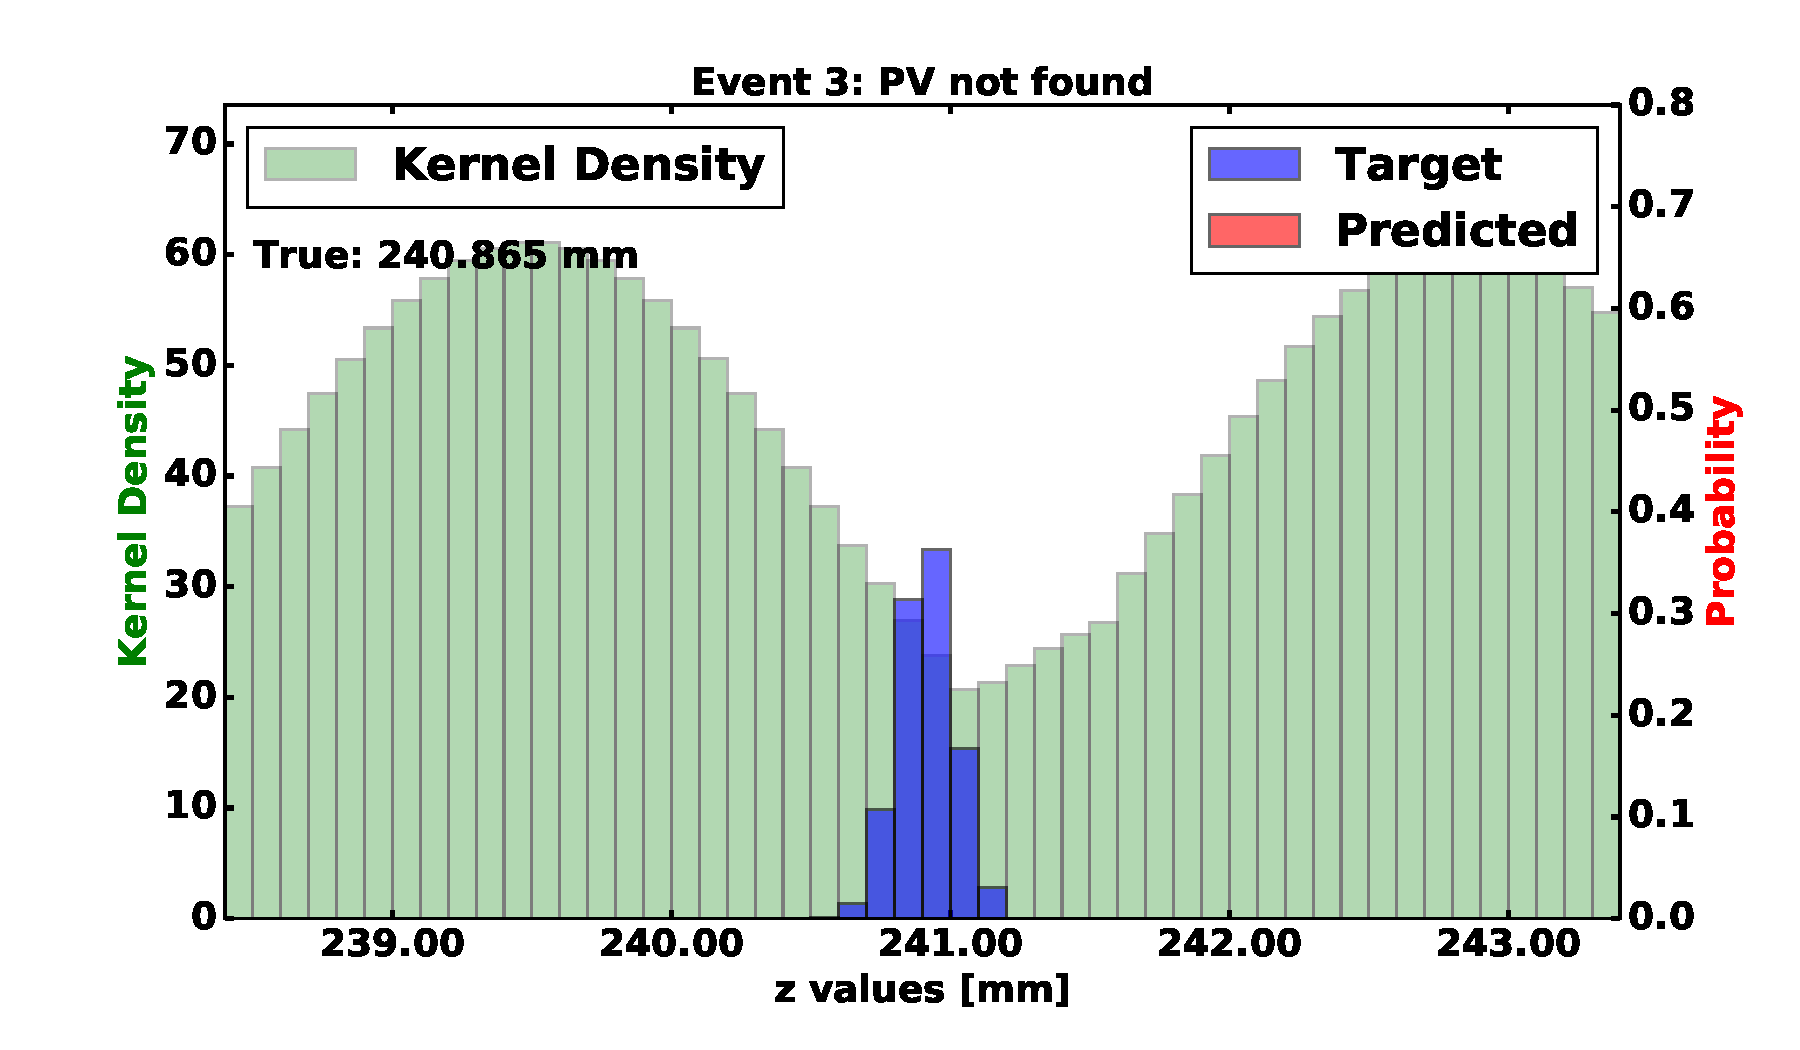
\includegraphics[width=1\textwidth, height=0.45\textwidth, trim=18 0 18 0]{images/120000_3layer_22.pdf}

           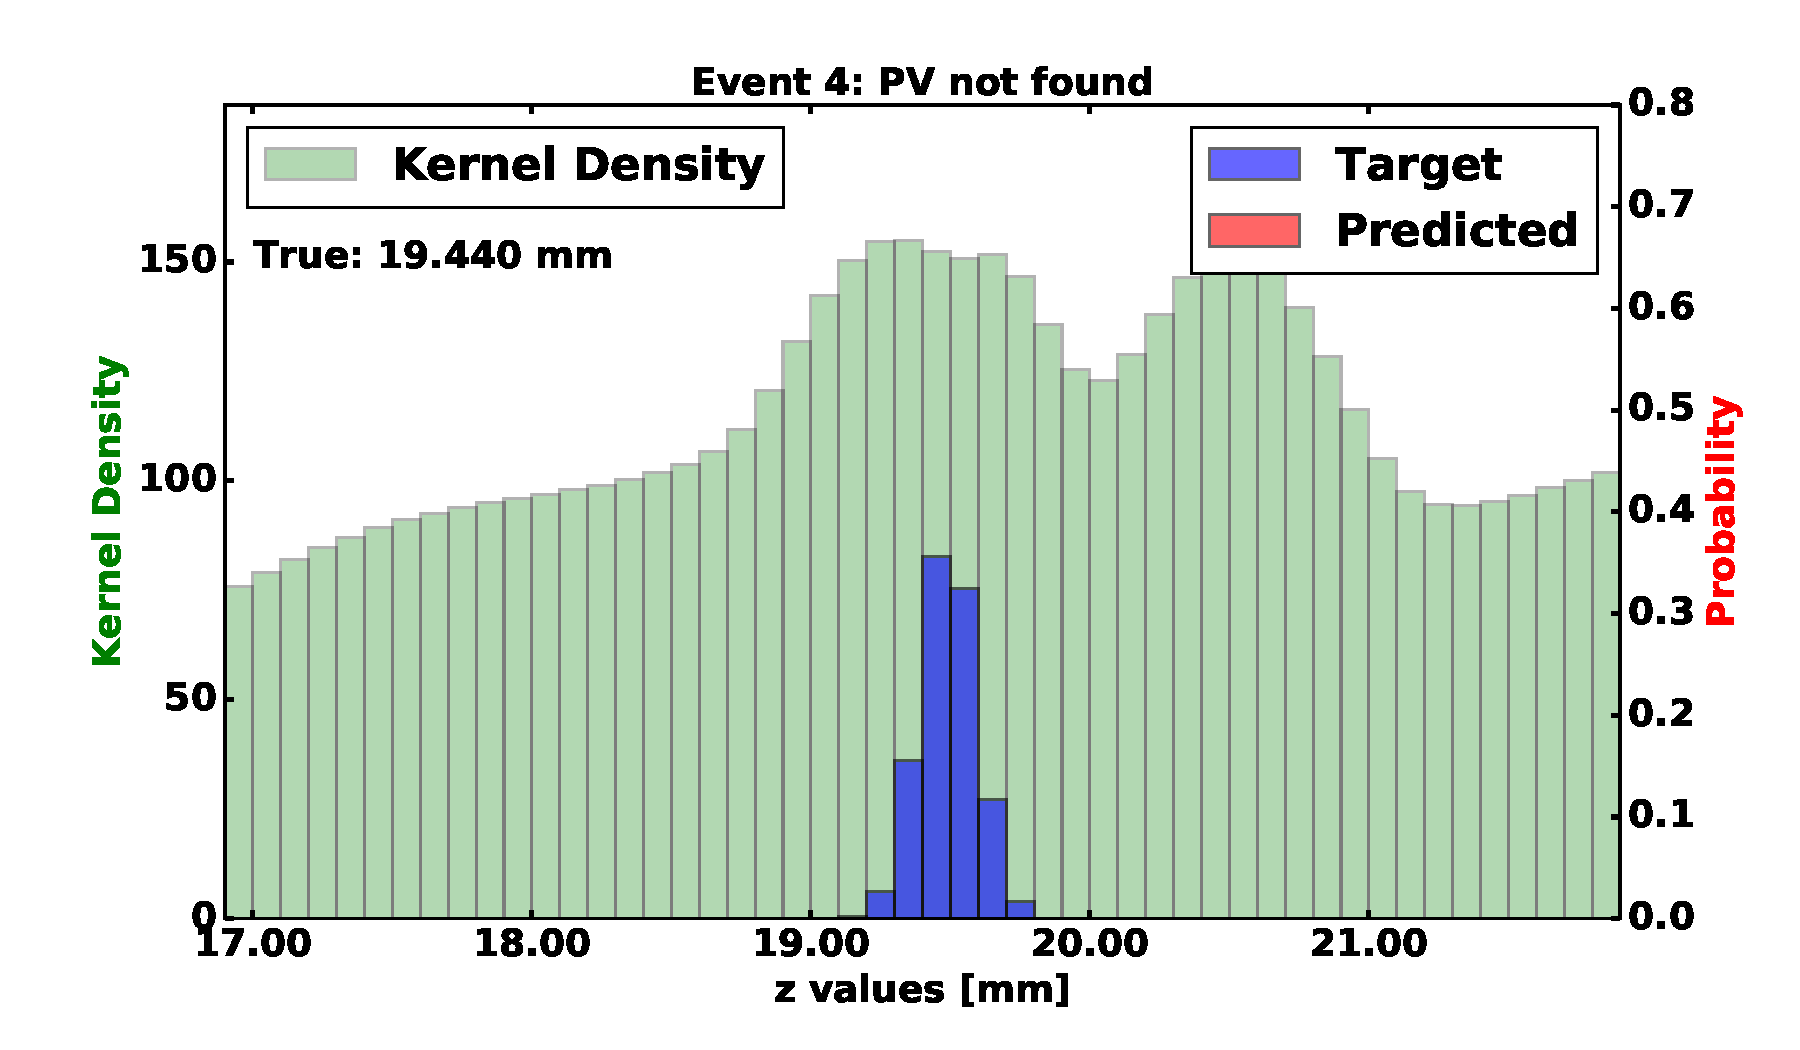
\includegraphics[width=1\textwidth, height=0.45\textwidth, trim=18 0 18 0]{images/120000_3layer_23.pdf}
       \end{center}
  \end{columns}
\end{frame}

\begin{frame}{More Predictions with Targets (3 CVN layers)}
  \begin{columns}[c]
    \column{.5\textwidth}
        \begin{center}
            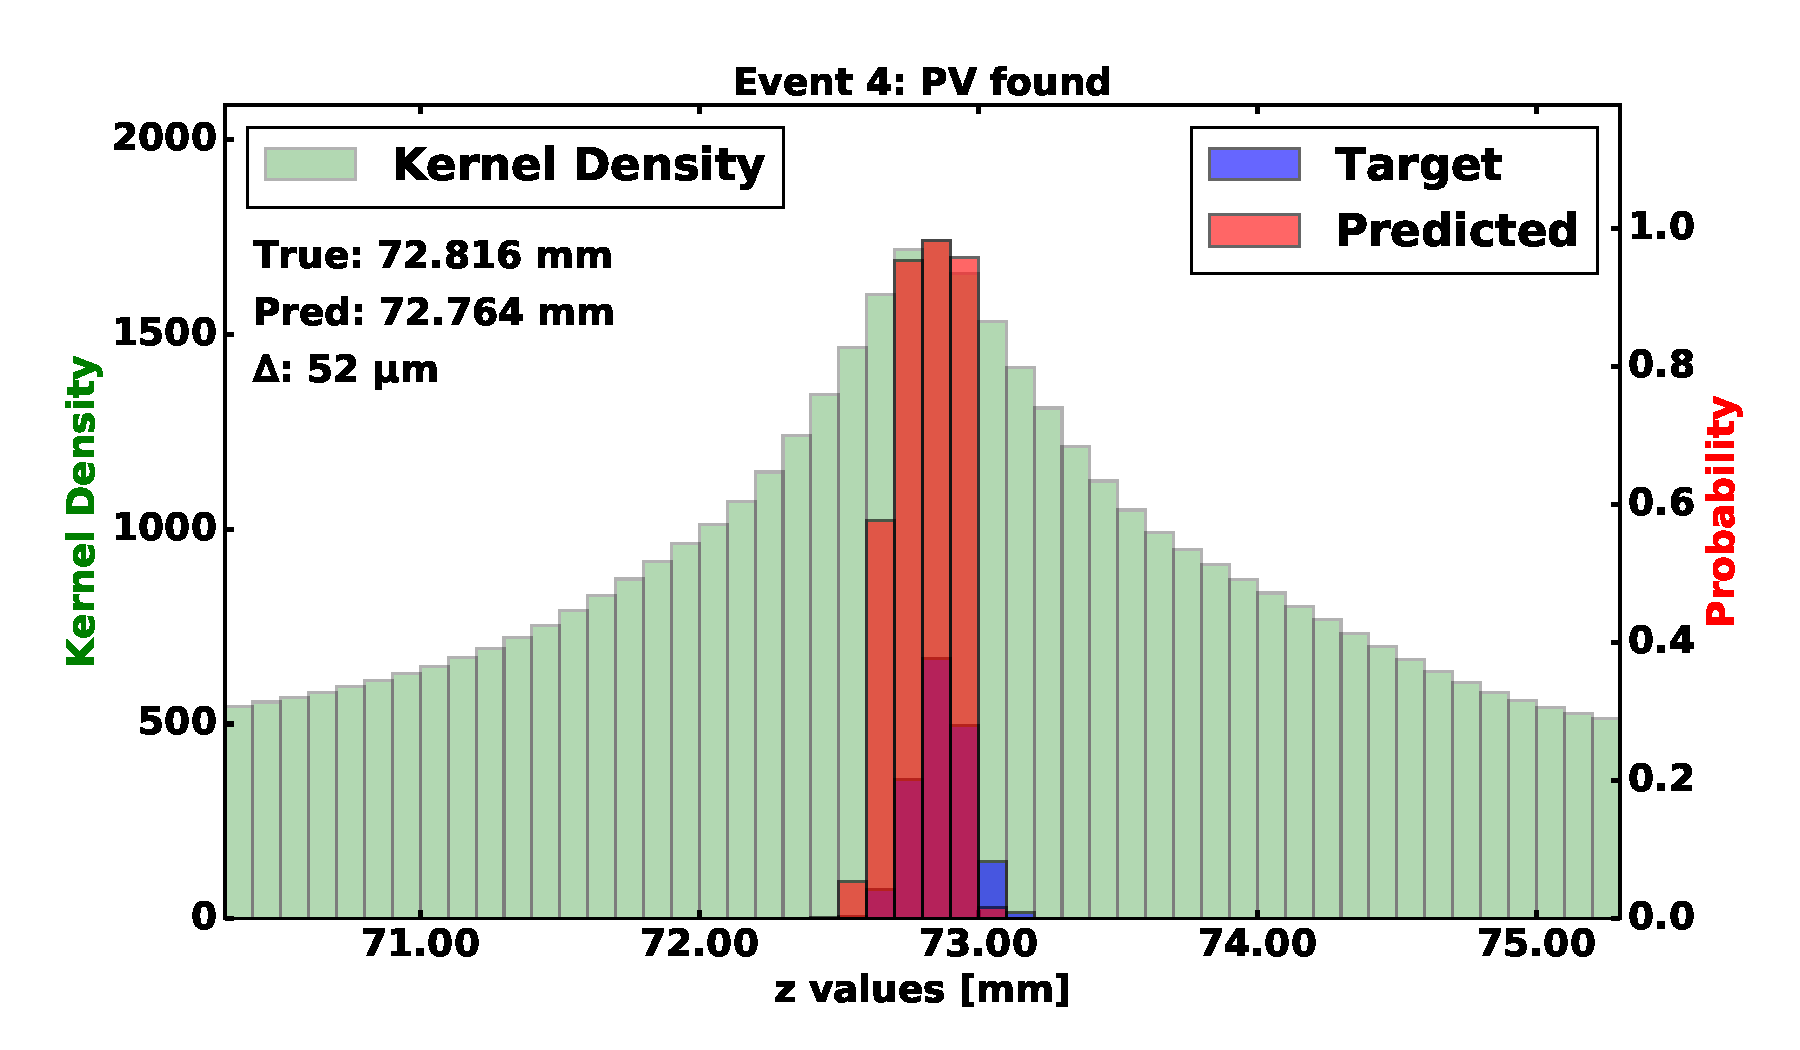
\includegraphics[width=1\textwidth,height=0.45\textwidth, trim=18 0 18 0]{images/120000_3layer_24.pdf}

            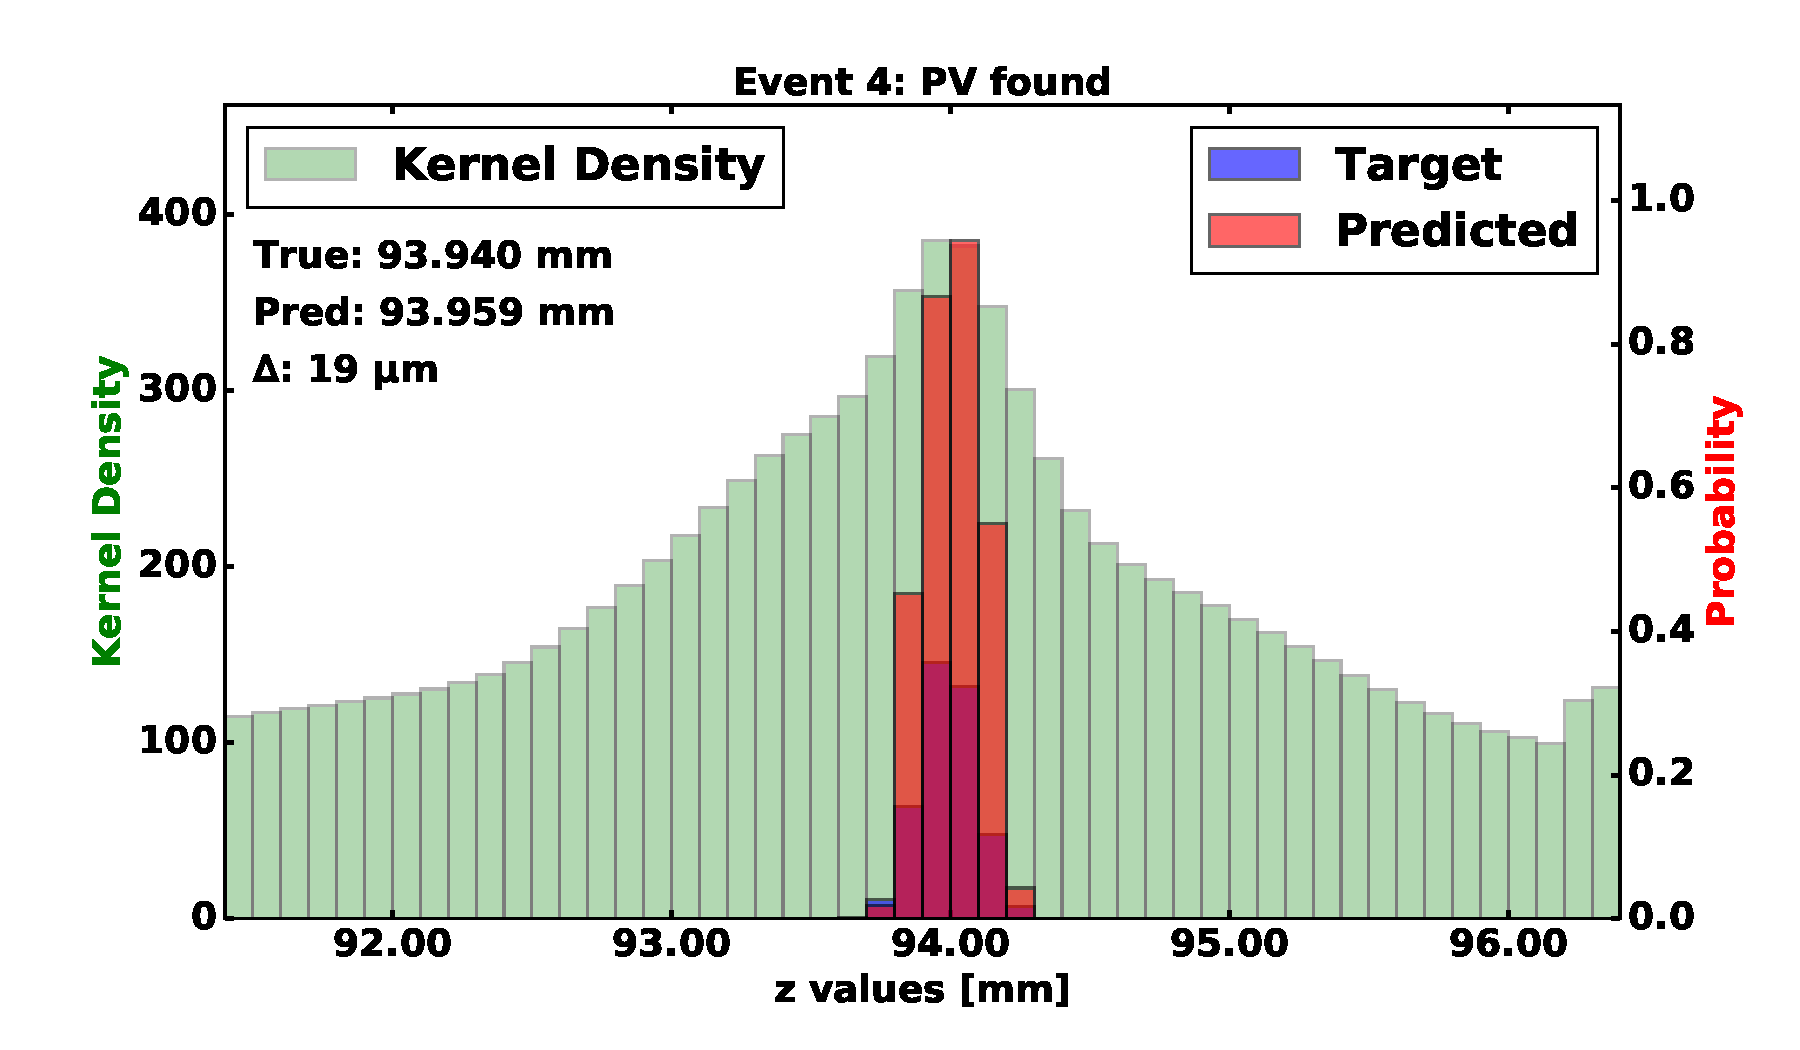
\includegraphics[width=1\textwidth, height=0.45\textwidth,trim=18 0 18 0]{images/120000_3layer_25.pdf}

        \end{center}
    \column{.5\textwidth}
        \begin{center}
           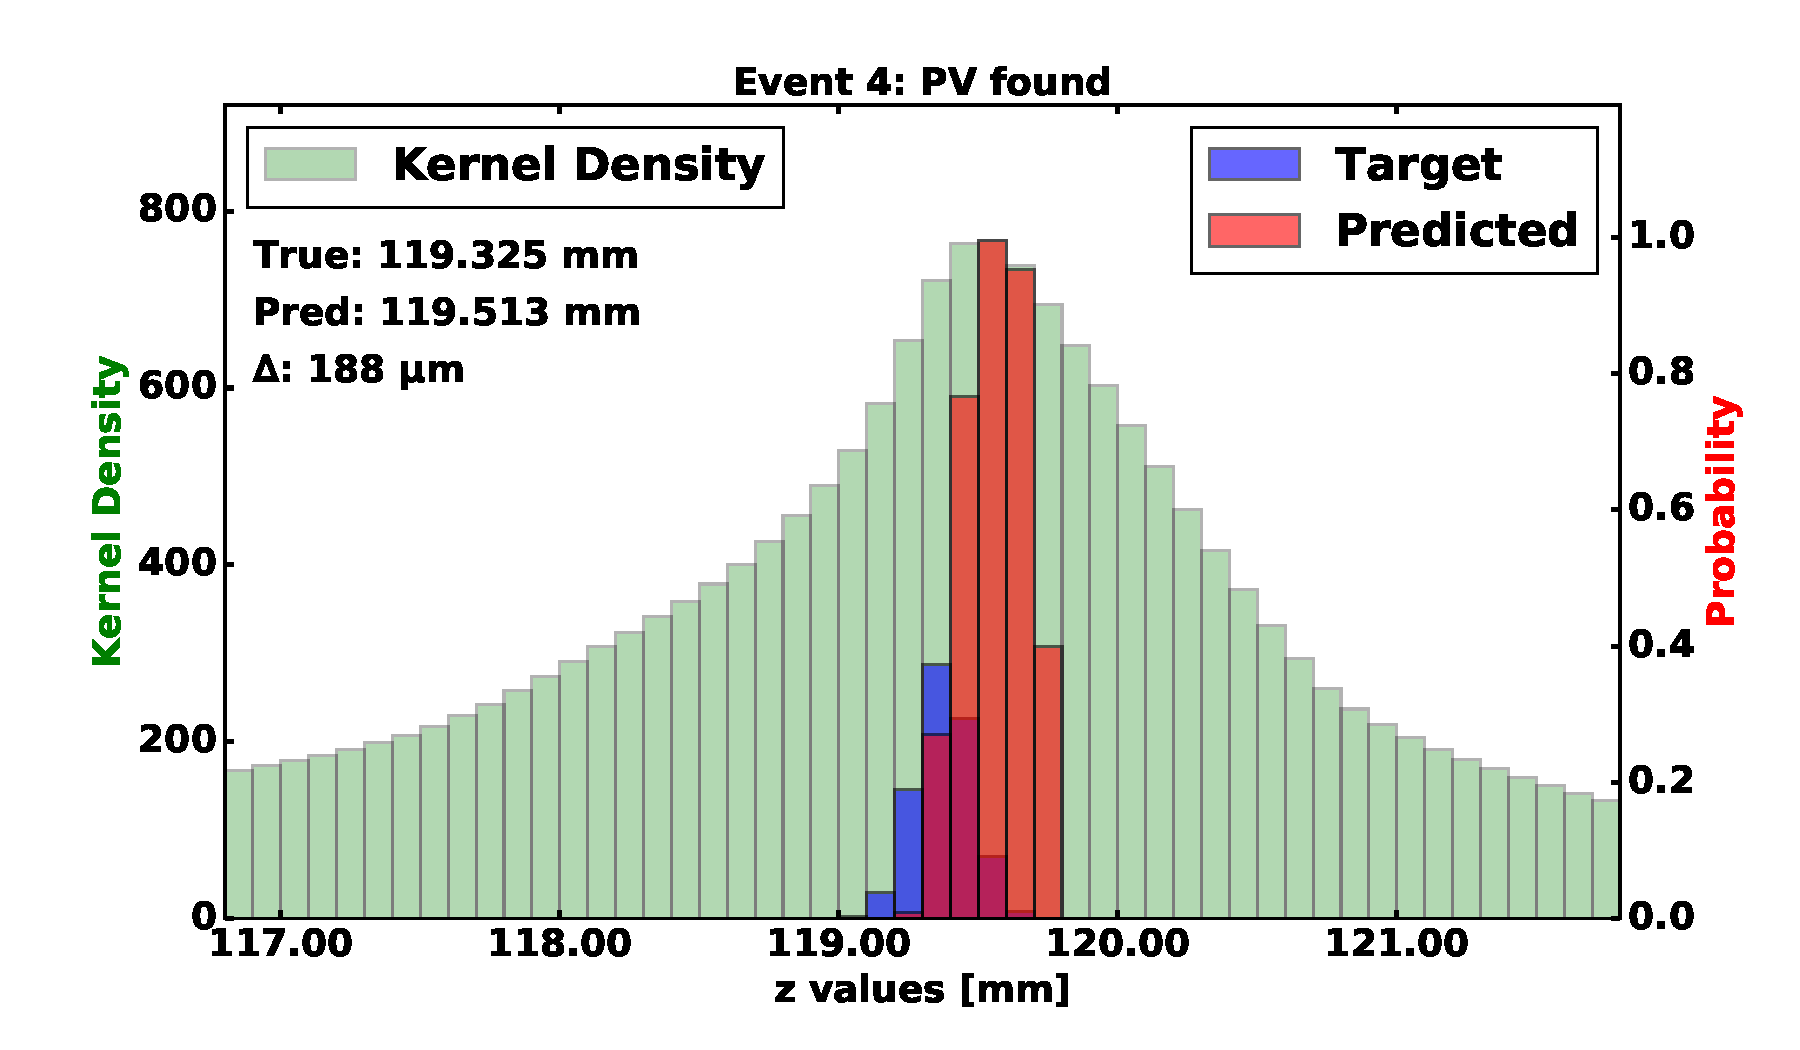
\includegraphics[width=1\textwidth, height=0.45\textwidth, trim=18 0 18 0]{images/120000_3layer_26.pdf}

           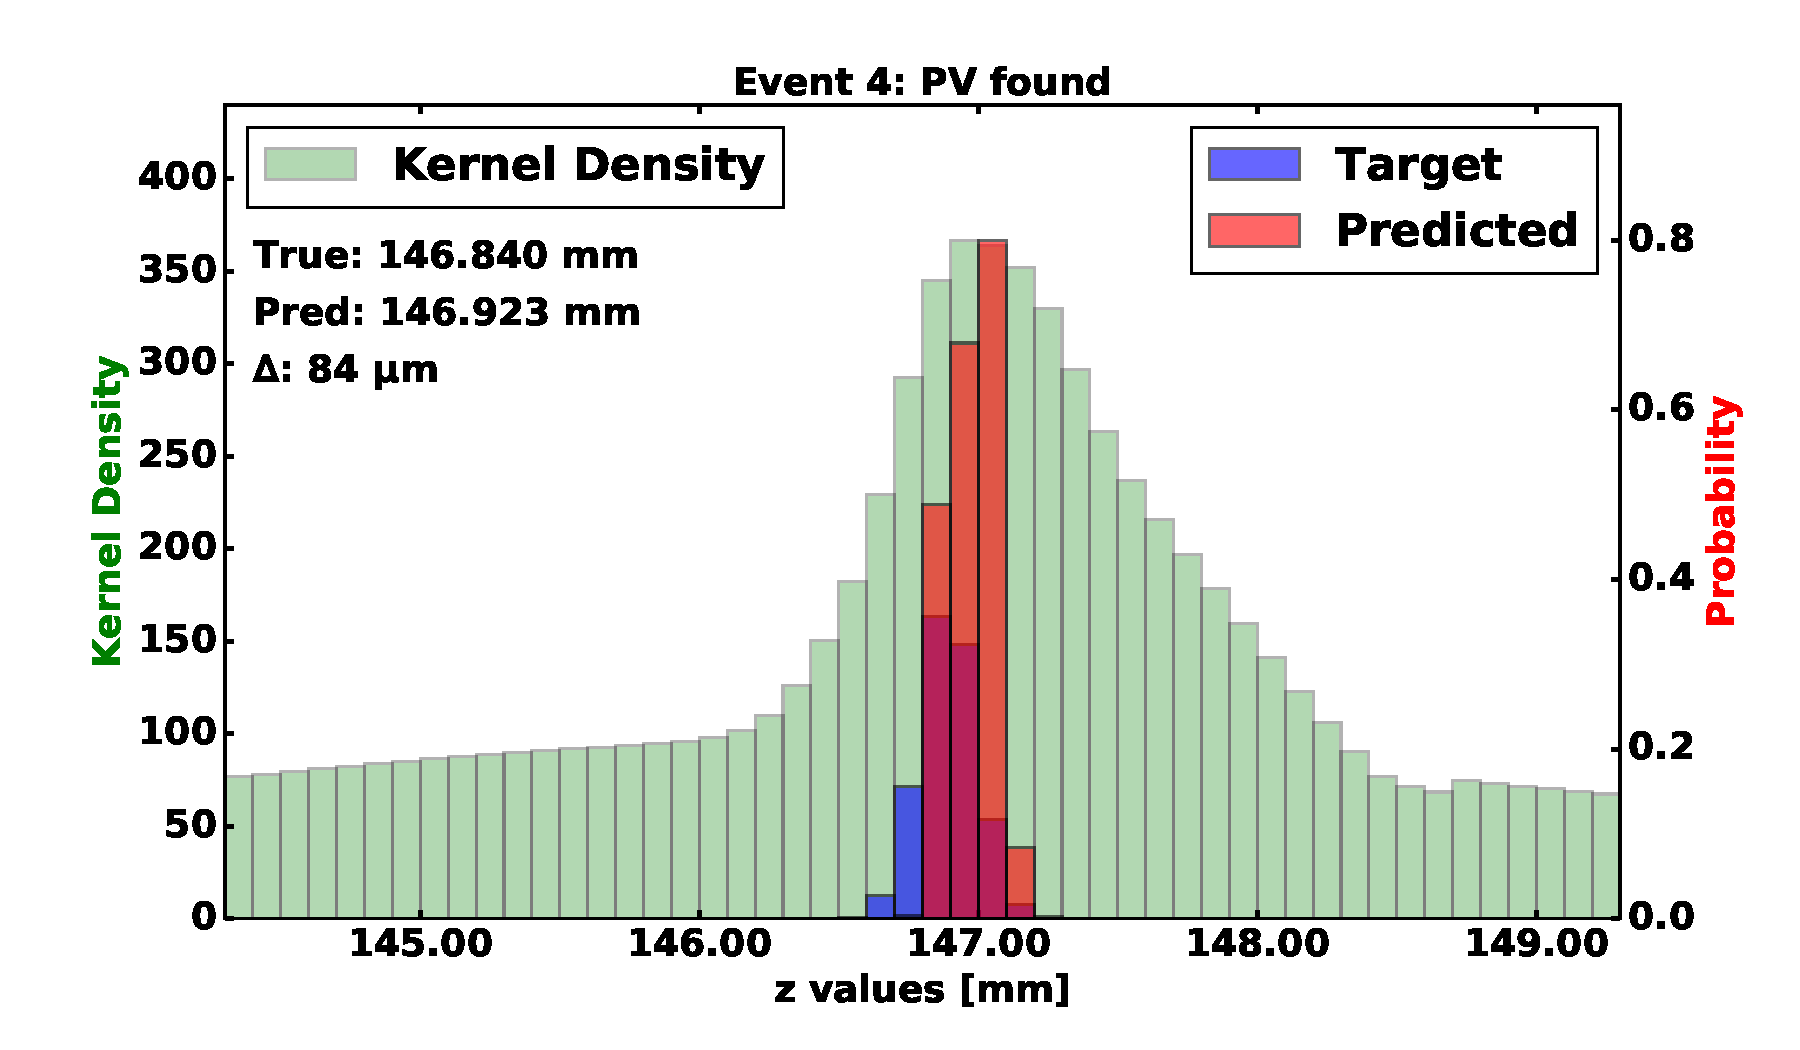
\includegraphics[width=1\textwidth, height=0.45\textwidth, trim=18 0 18 0]{images/120000_3layer_27.pdf}
       \end{center}
  \end{columns}
\end{frame}

\begin{frame}{More Predictions with Targets (3 CVN layers)}
  \begin{columns}[c]
    \column{.5\textwidth}
        \begin{center}
            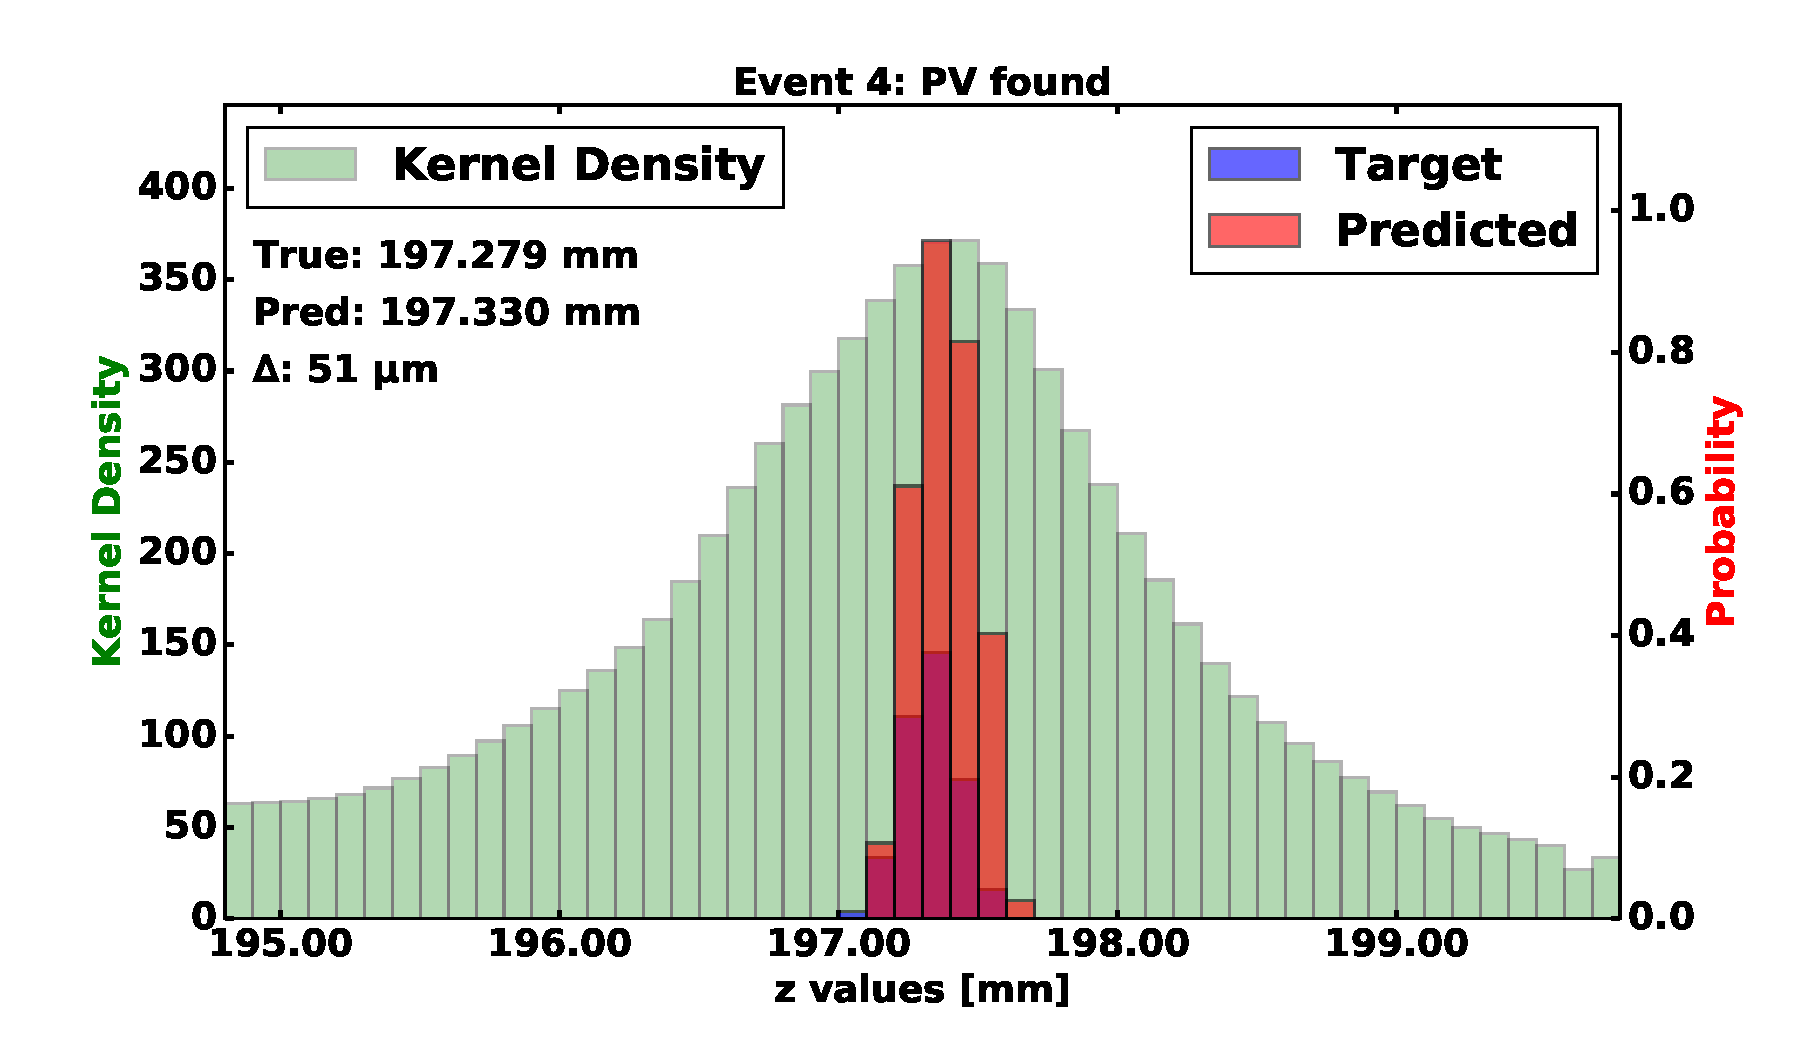
\includegraphics[width=1\textwidth,height=0.45\textwidth, trim=18 0 18 0]{images/120000_3layer_28.pdf}

            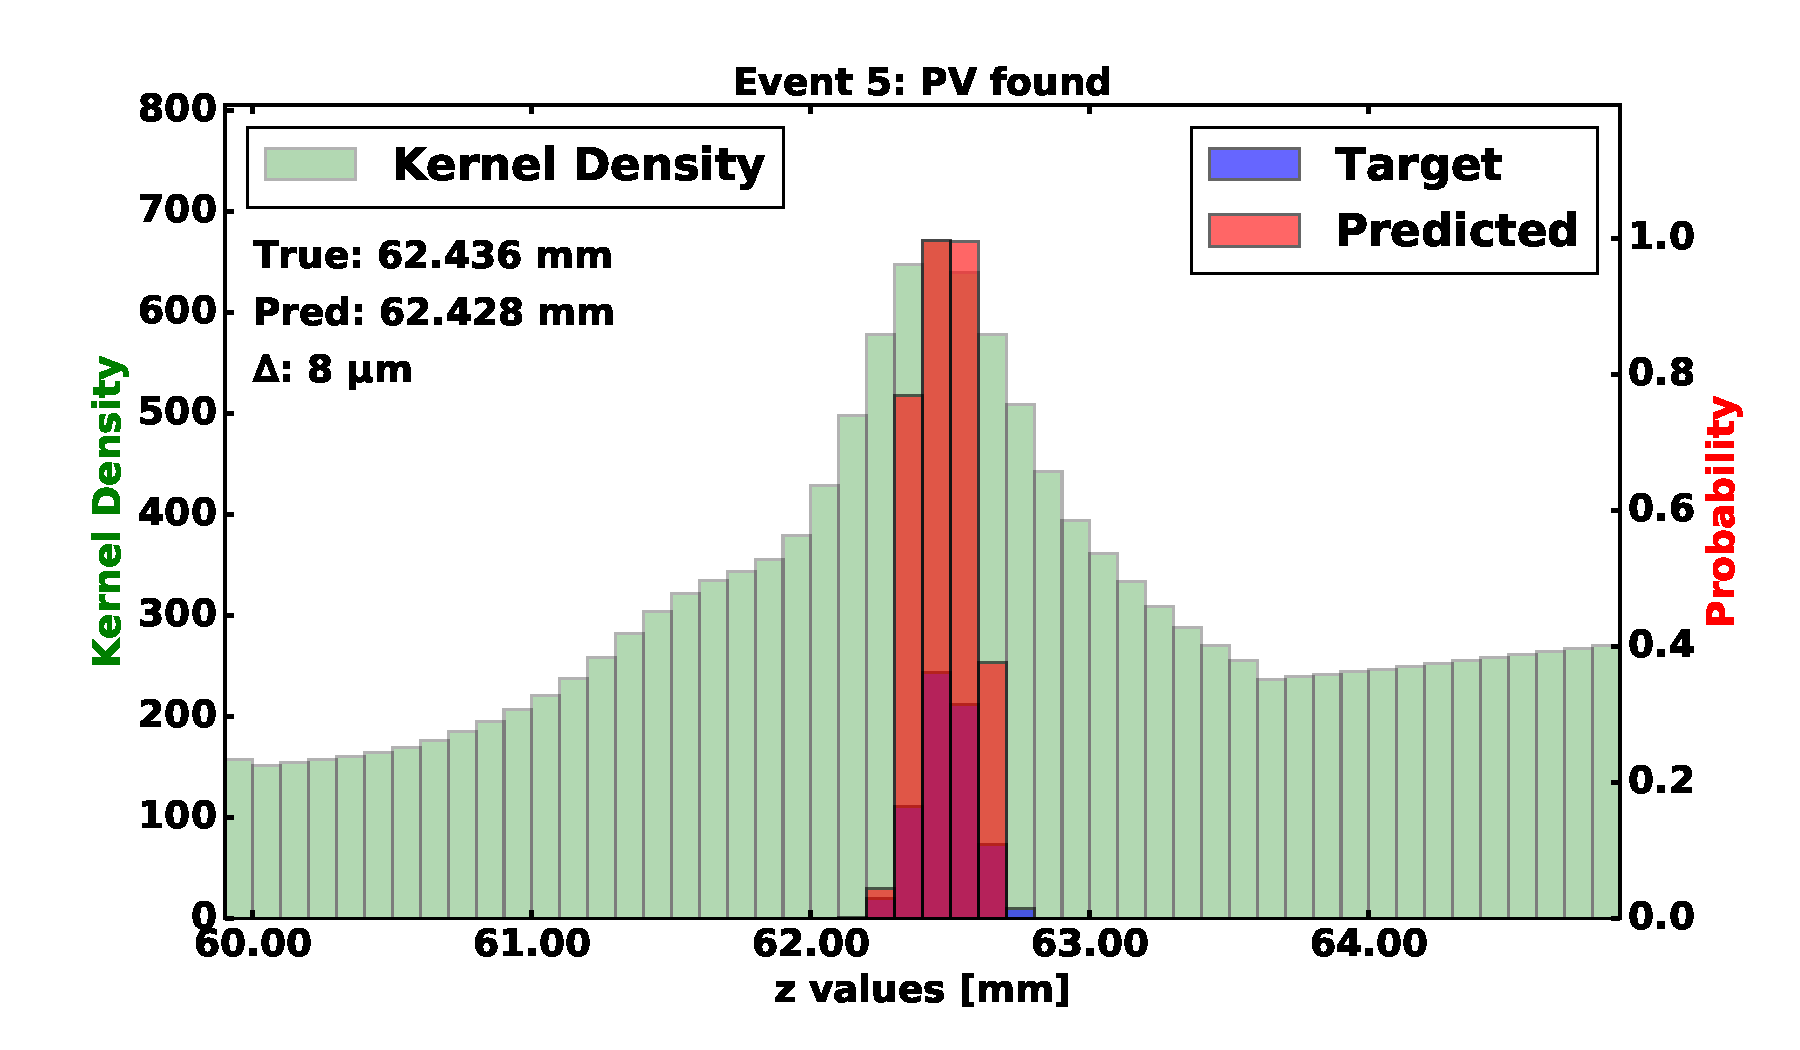
\includegraphics[width=1\textwidth, height=0.45\textwidth,trim=18 0 18 0]{images/120000_3layer_29.pdf}

        \end{center}
    \column{.5\textwidth}
        \begin{center}
           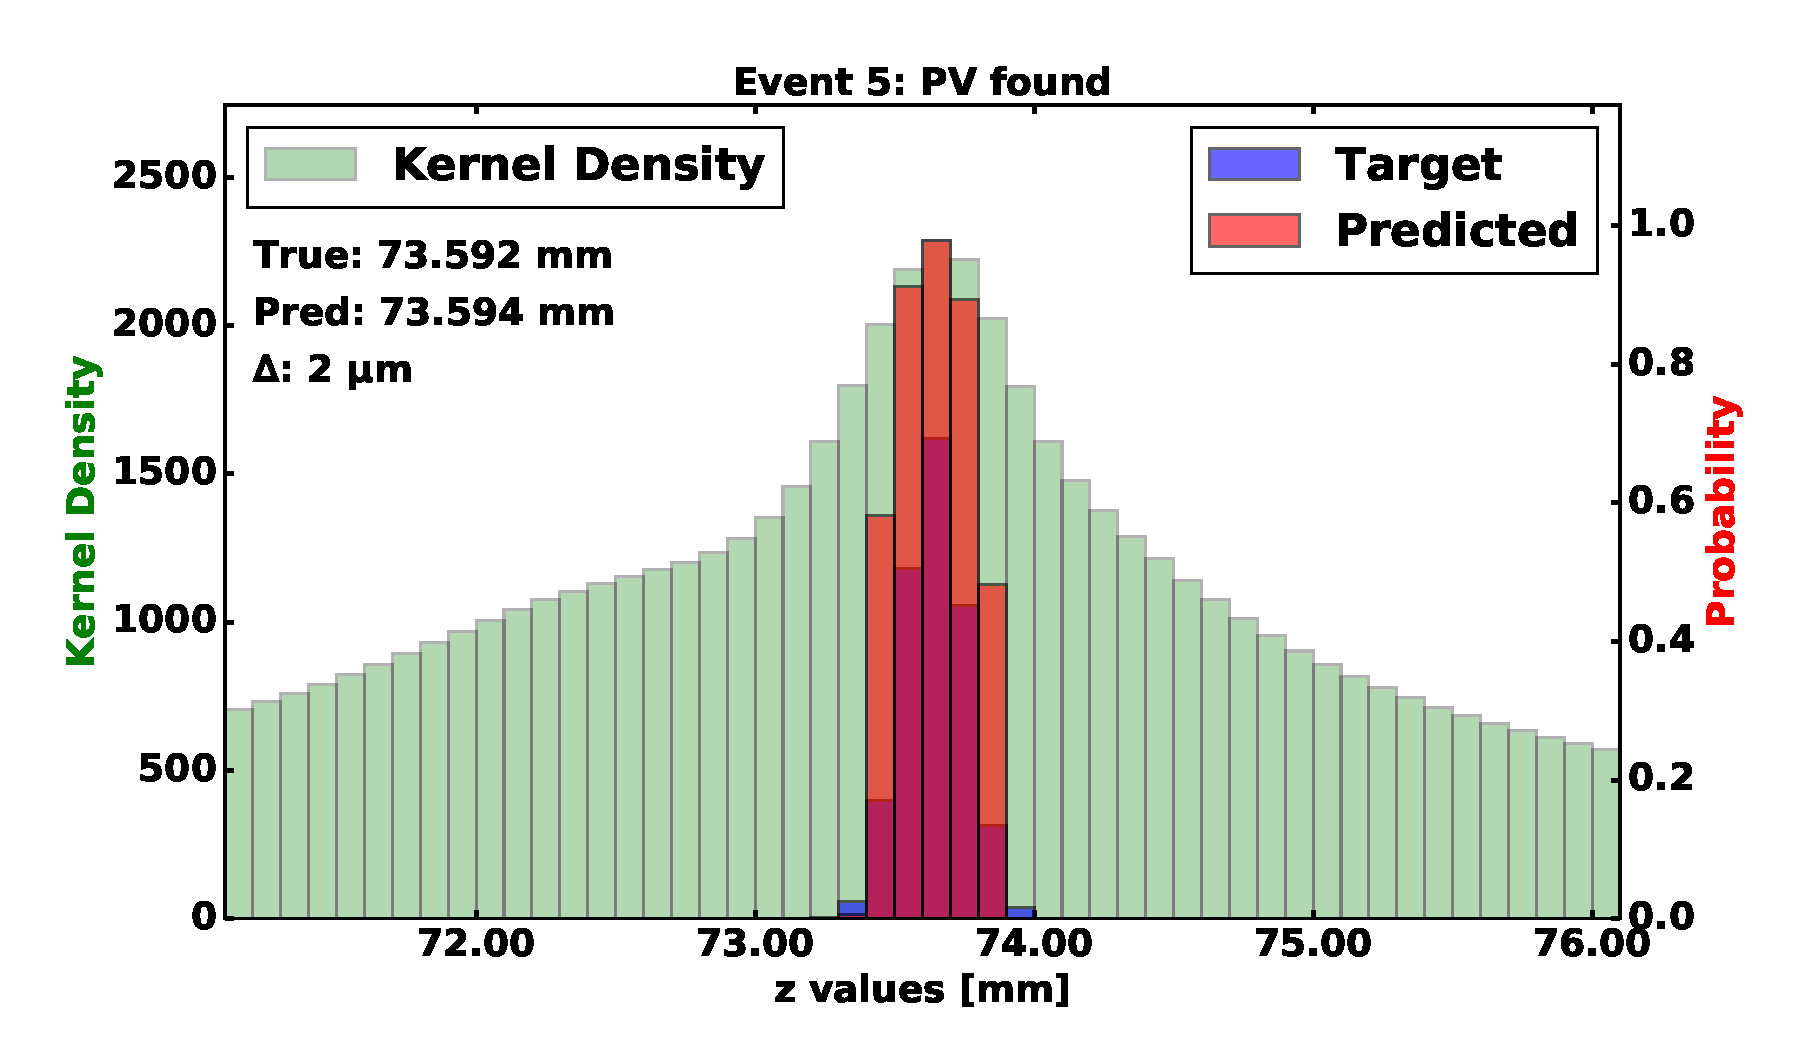
\includegraphics[width=1\textwidth, height=0.45\textwidth, trim=18 0 18 0]{images/120000_3layer_30.pdf}

           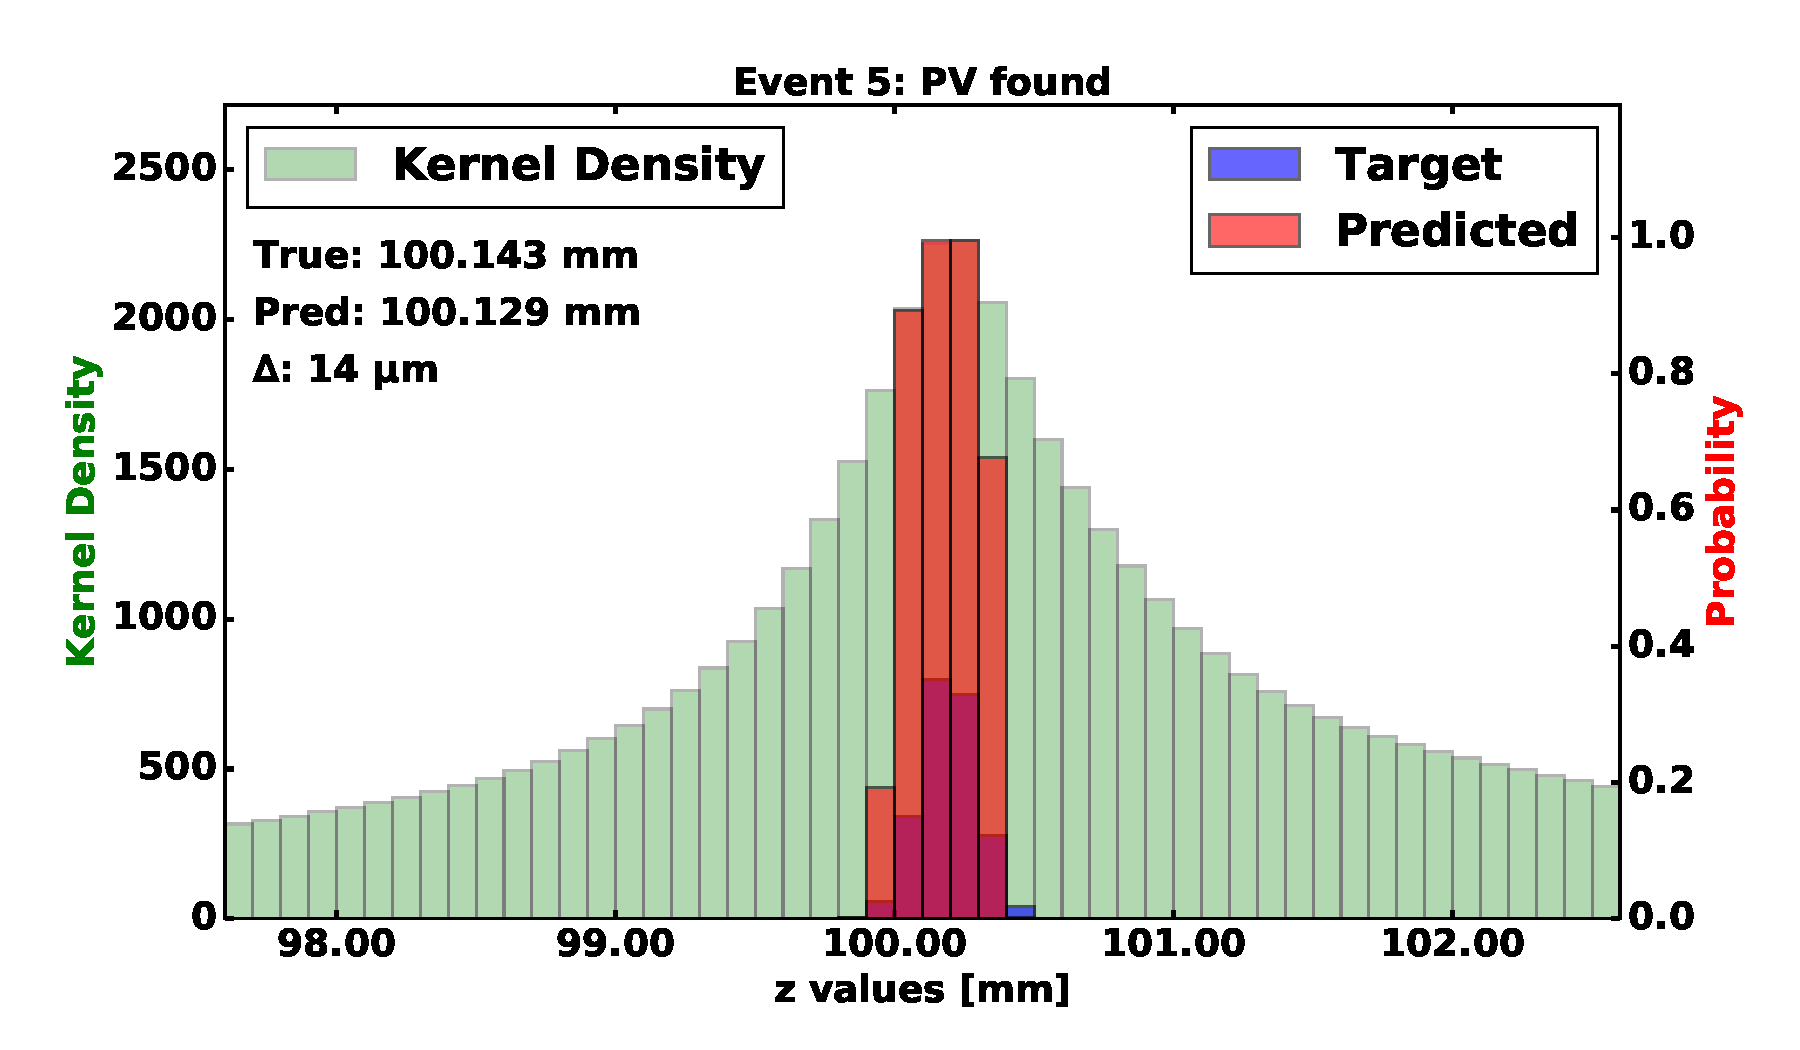
\includegraphics[width=1\textwidth, height=0.45\textwidth, trim=18 0 18 0]{images/120000_3layer_31.pdf}
       \end{center}
  \end{columns}
\end{frame}

\begin{frame}{More Predictions with Targets (3 CVN layers)}
  \begin{columns}[c]
    \column{.5\textwidth}
        \begin{center}
            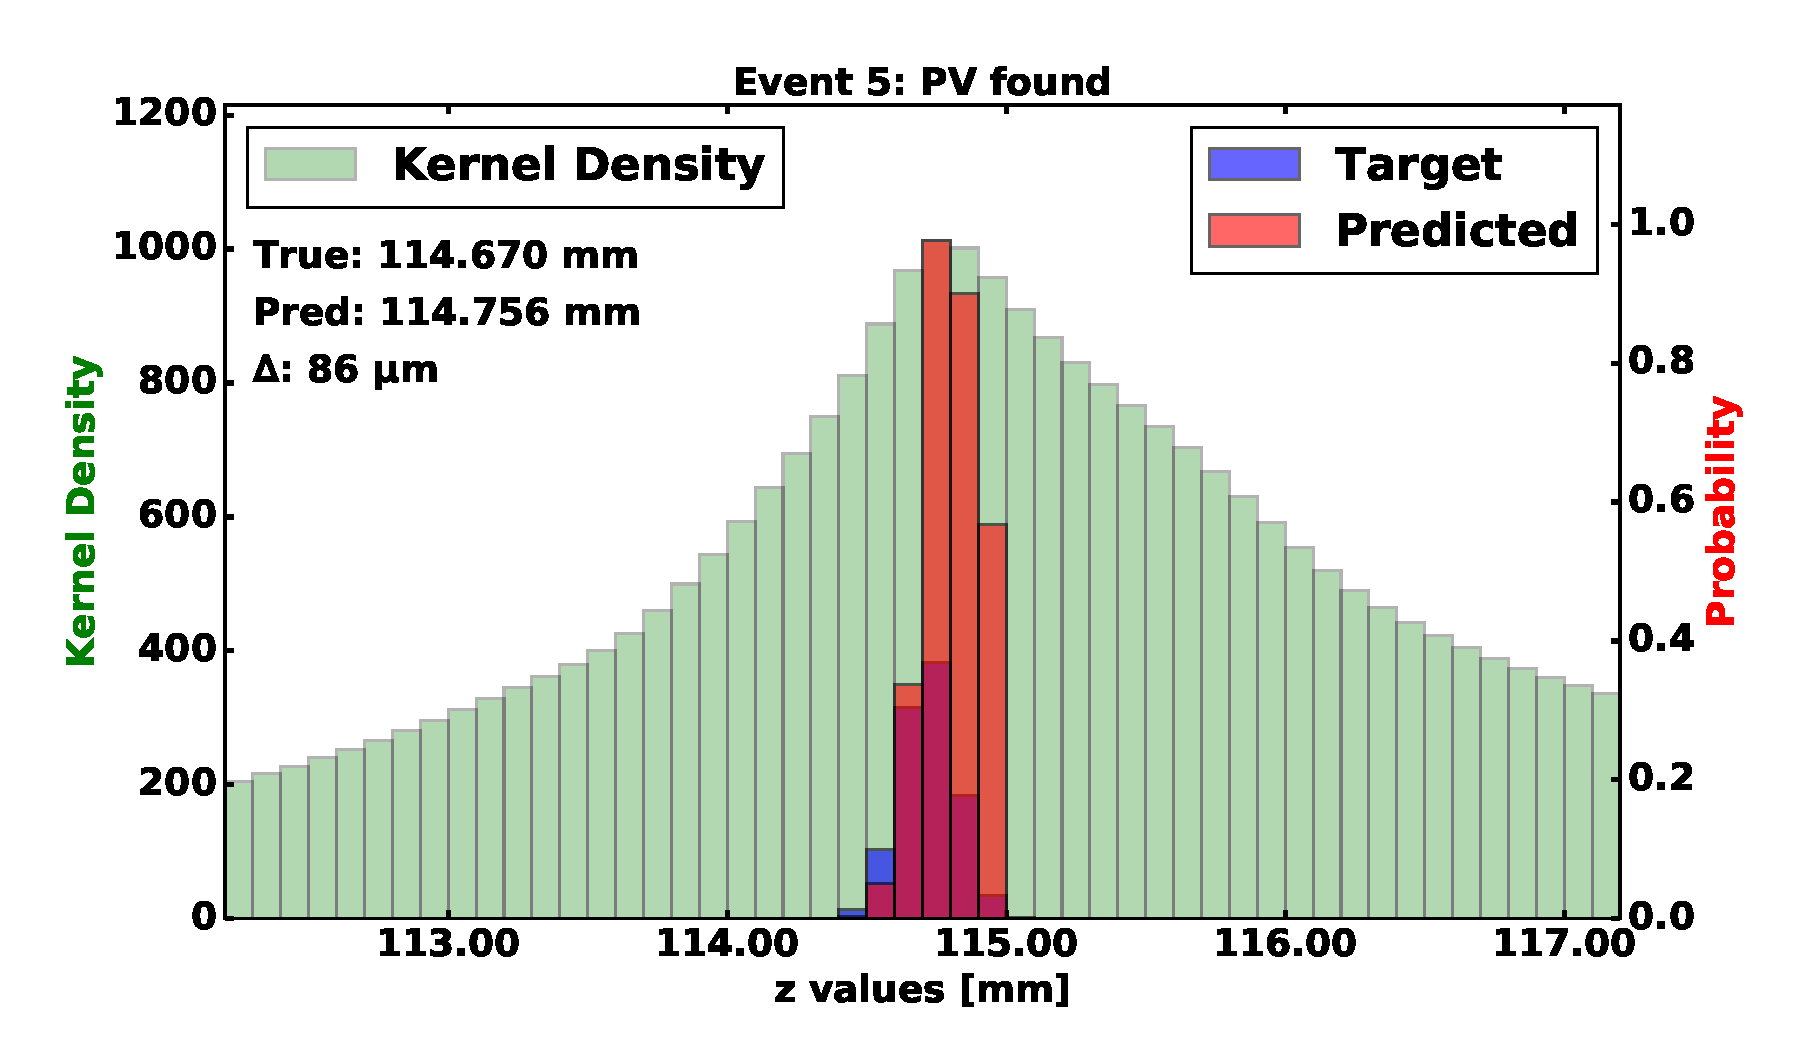
\includegraphics[width=1\textwidth,height=0.45\textwidth, trim=18 0 18 0]{images/120000_3layer_32.pdf}

            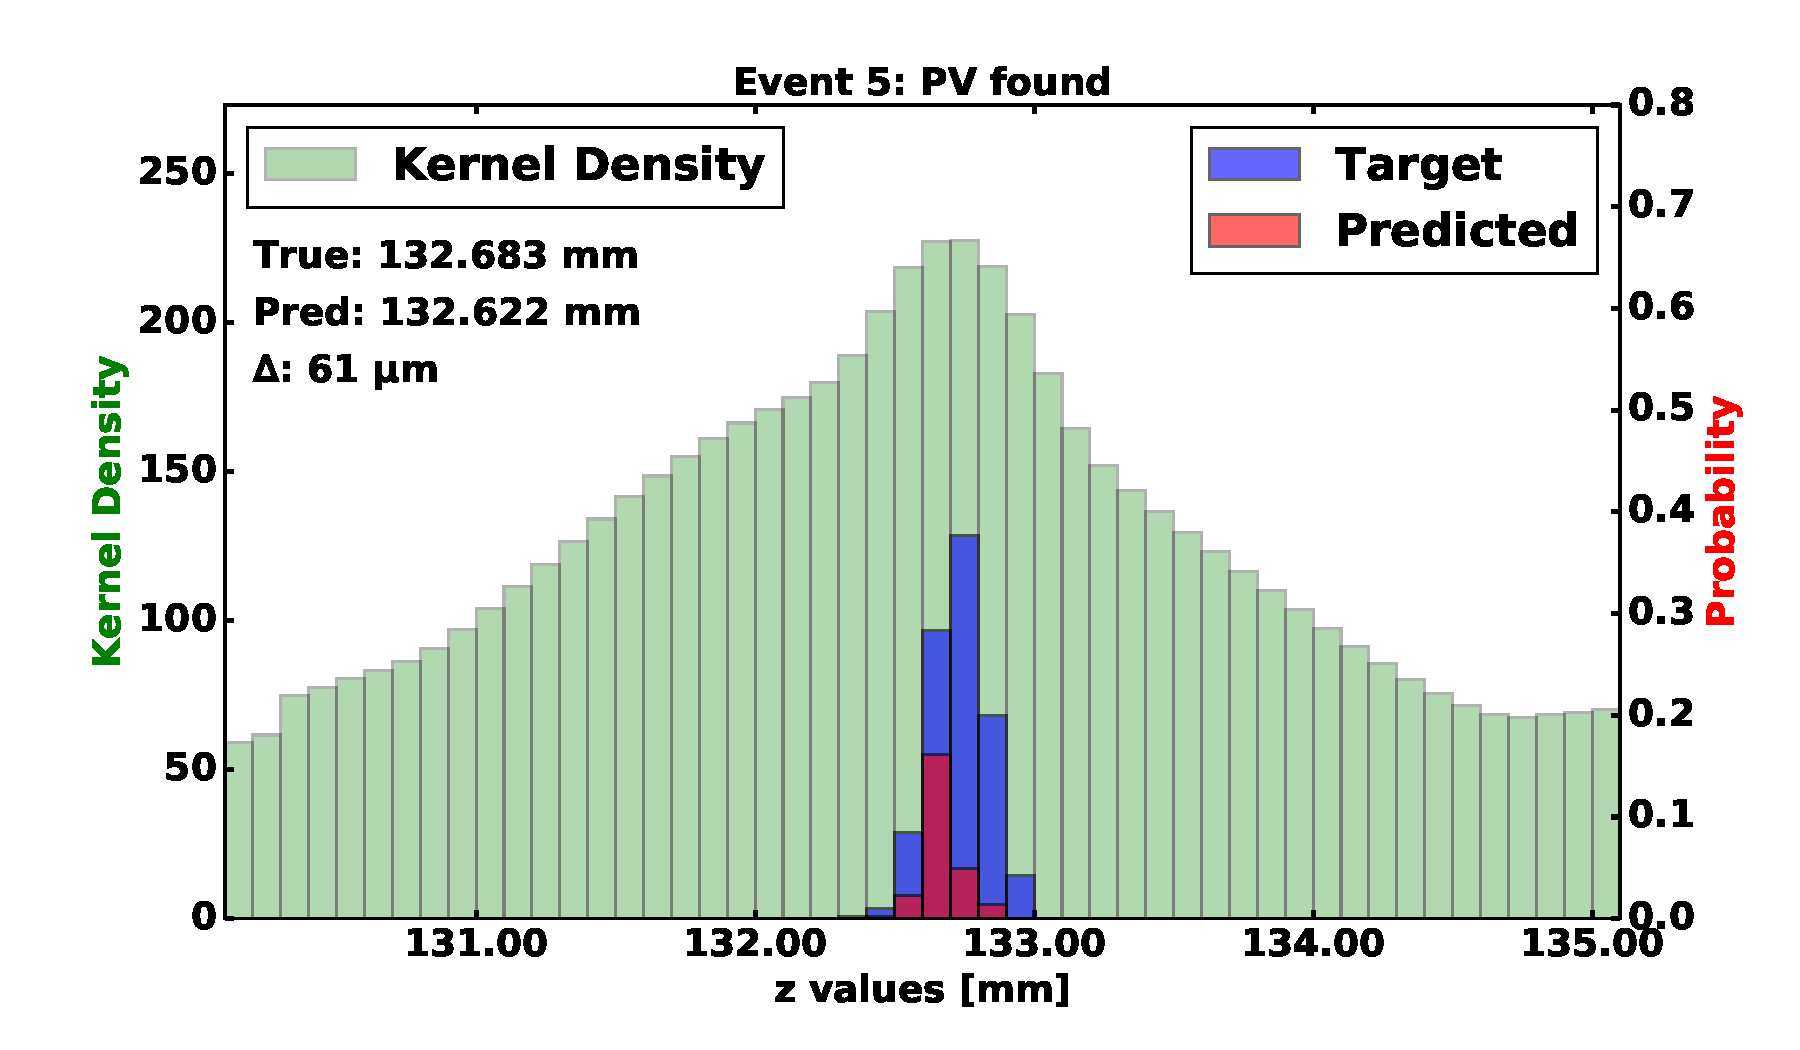
\includegraphics[width=1\textwidth, height=0.45\textwidth,trim=18 0 18 0]{images/120000_3layer_33.pdf}

        \end{center}
    \column{.5\textwidth}
        \begin{center}
           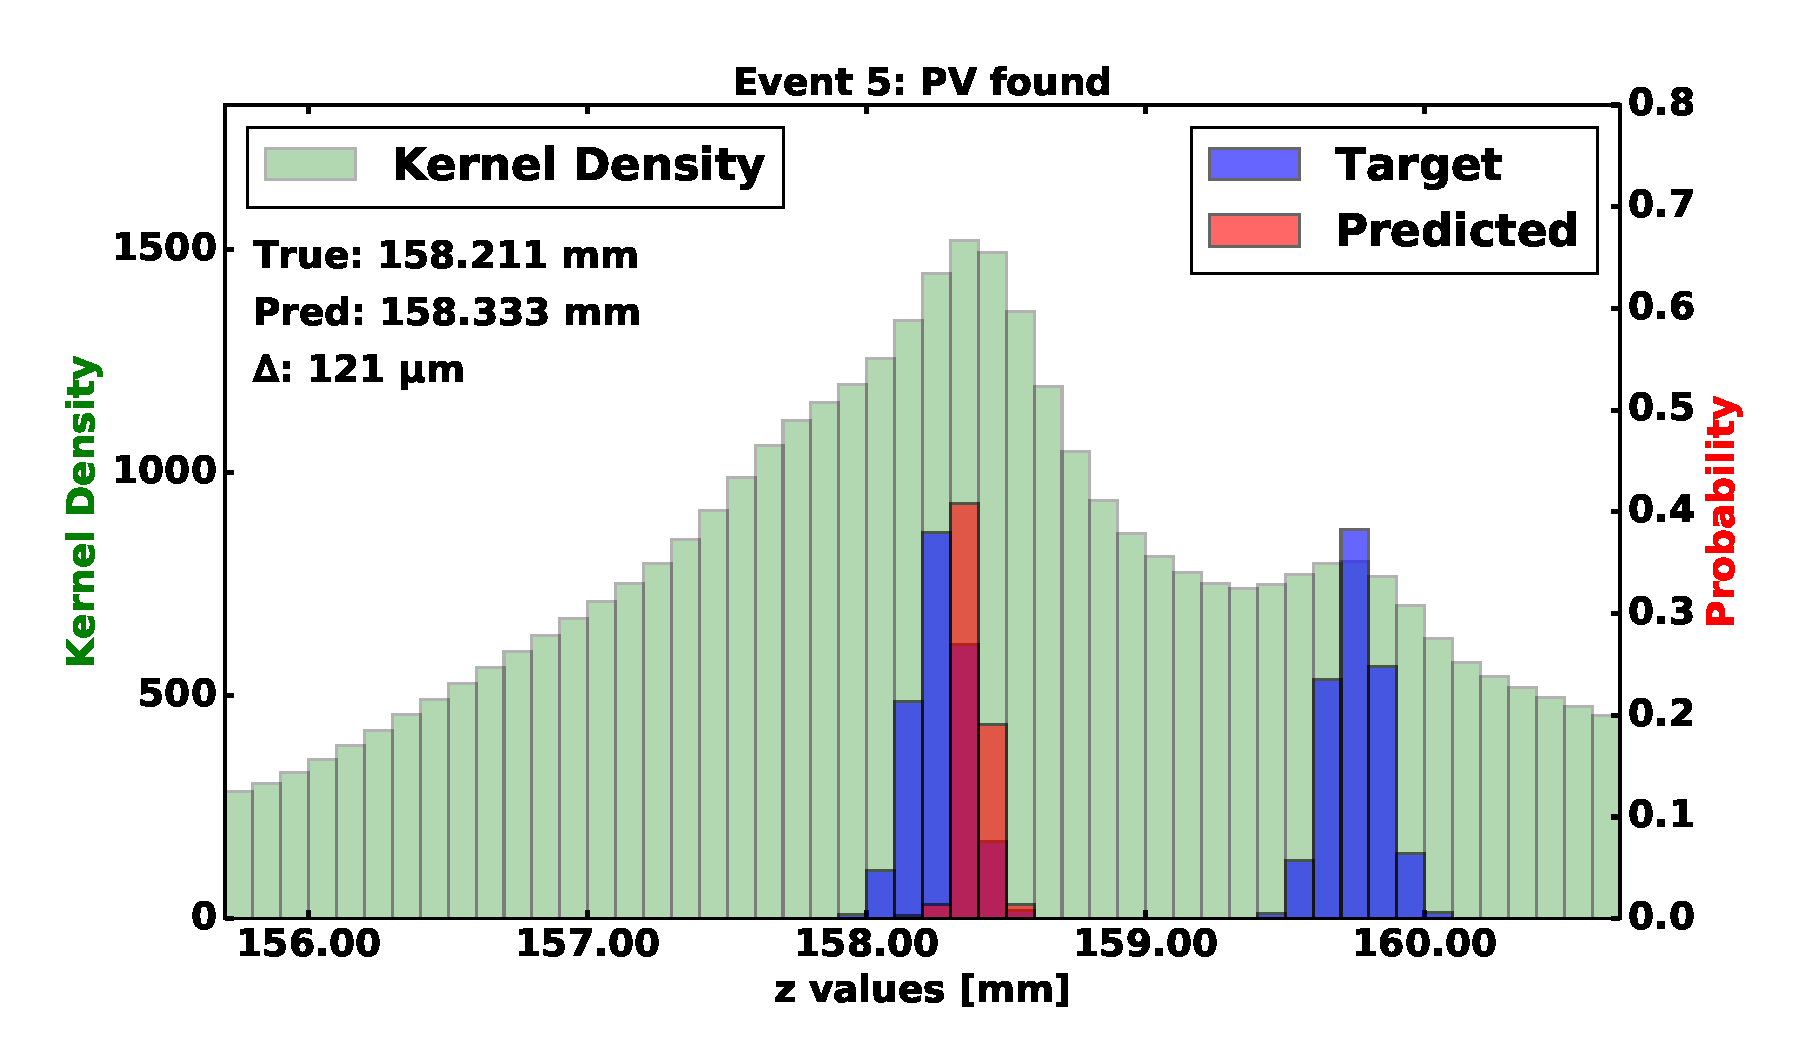
\includegraphics[width=1\textwidth, height=0.45\textwidth, trim=18 0 18 0]{images/120000_3layer_34.pdf}

           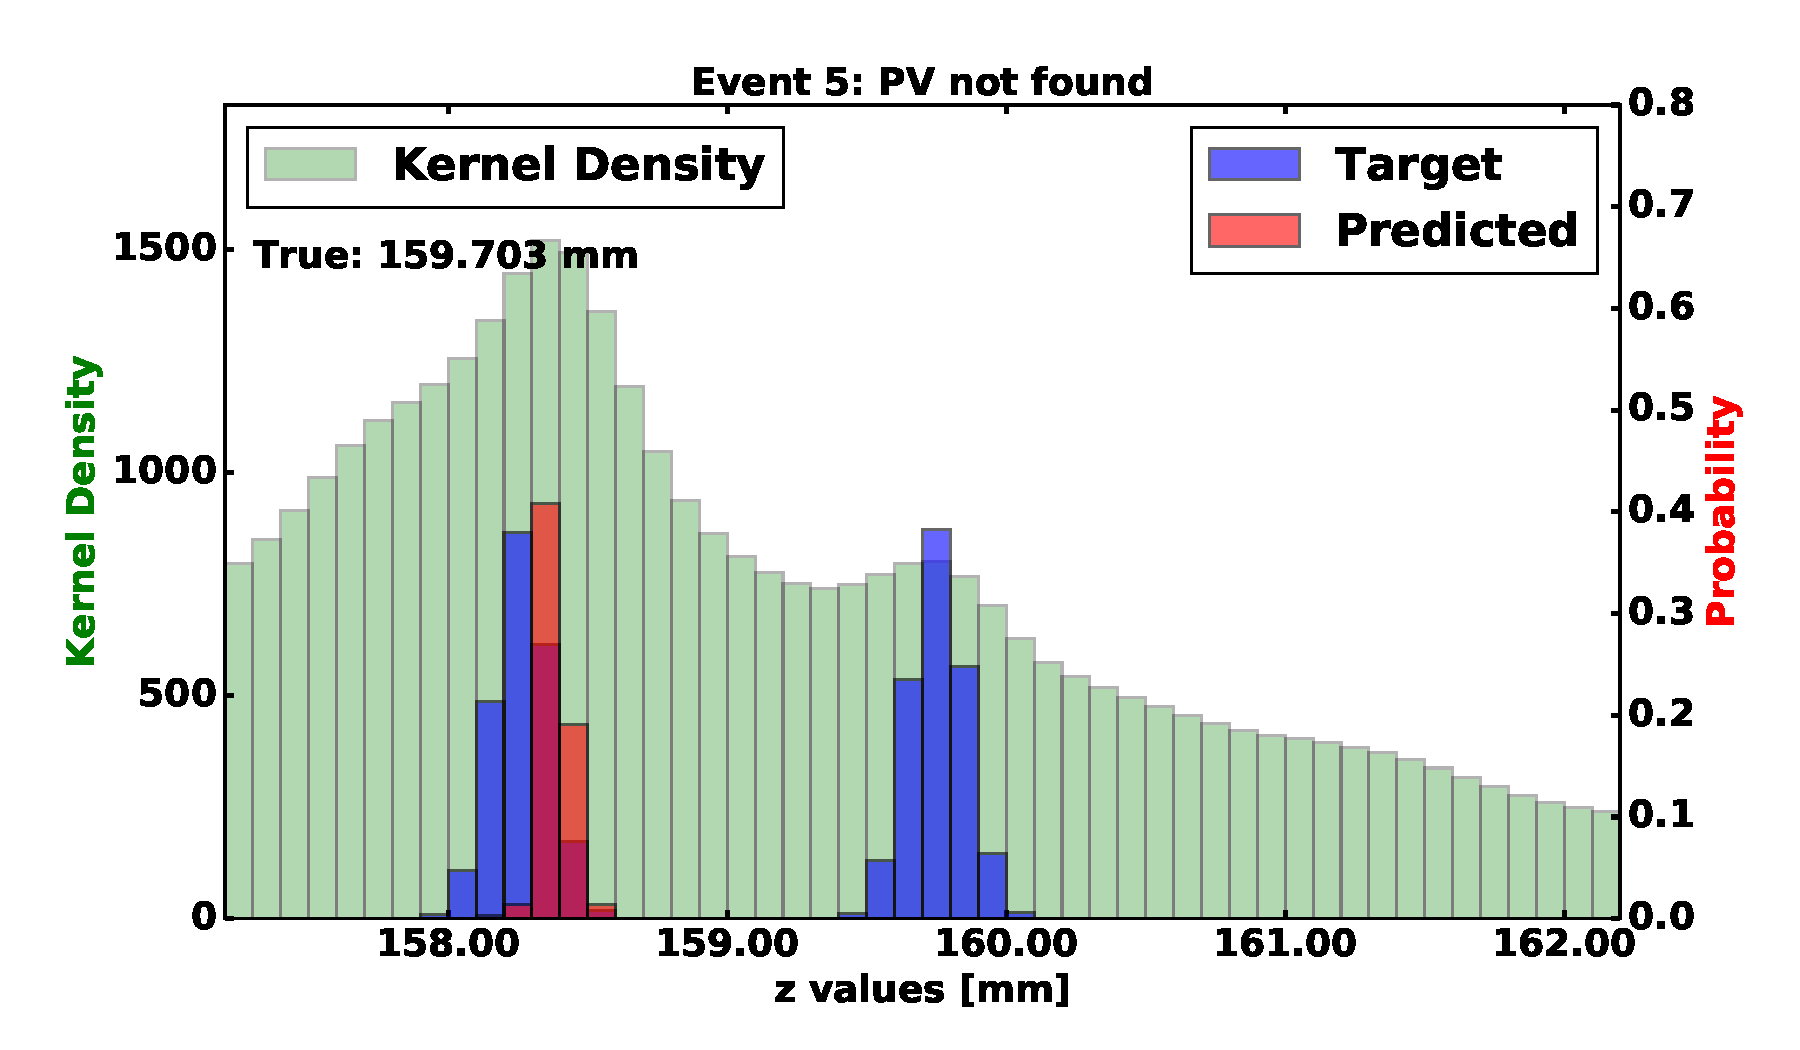
\includegraphics[width=1\textwidth, height=0.45\textwidth, trim=18 0 18 0]{images/120000_3layer_35.pdf}
       \end{center}
  \end{columns}
\end{frame}

\begin{frame}{More Predictions with Targets (3 CVN layers)}
  \begin{columns}[c]
    \column{.5\textwidth}
        \begin{center}
            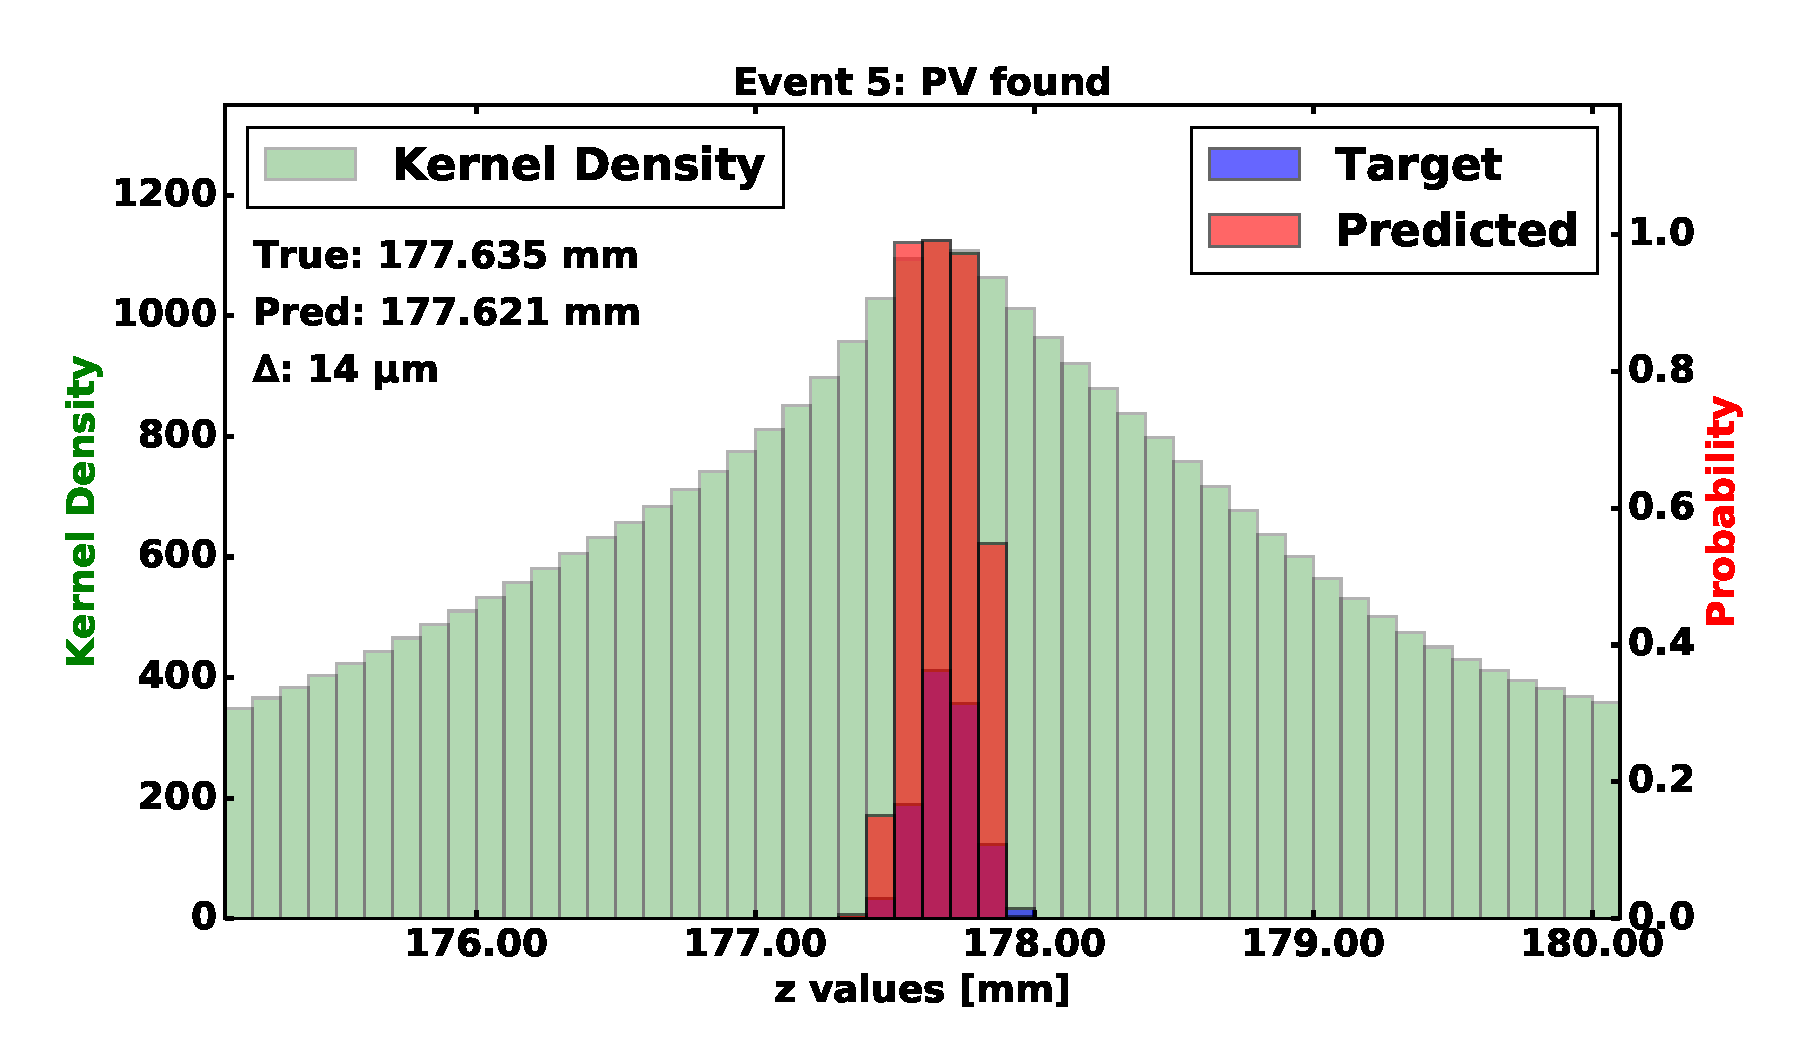
\includegraphics[width=1\textwidth,height=0.45\textwidth, trim=18 0 18 0]{images/120000_3layer_36.pdf}

            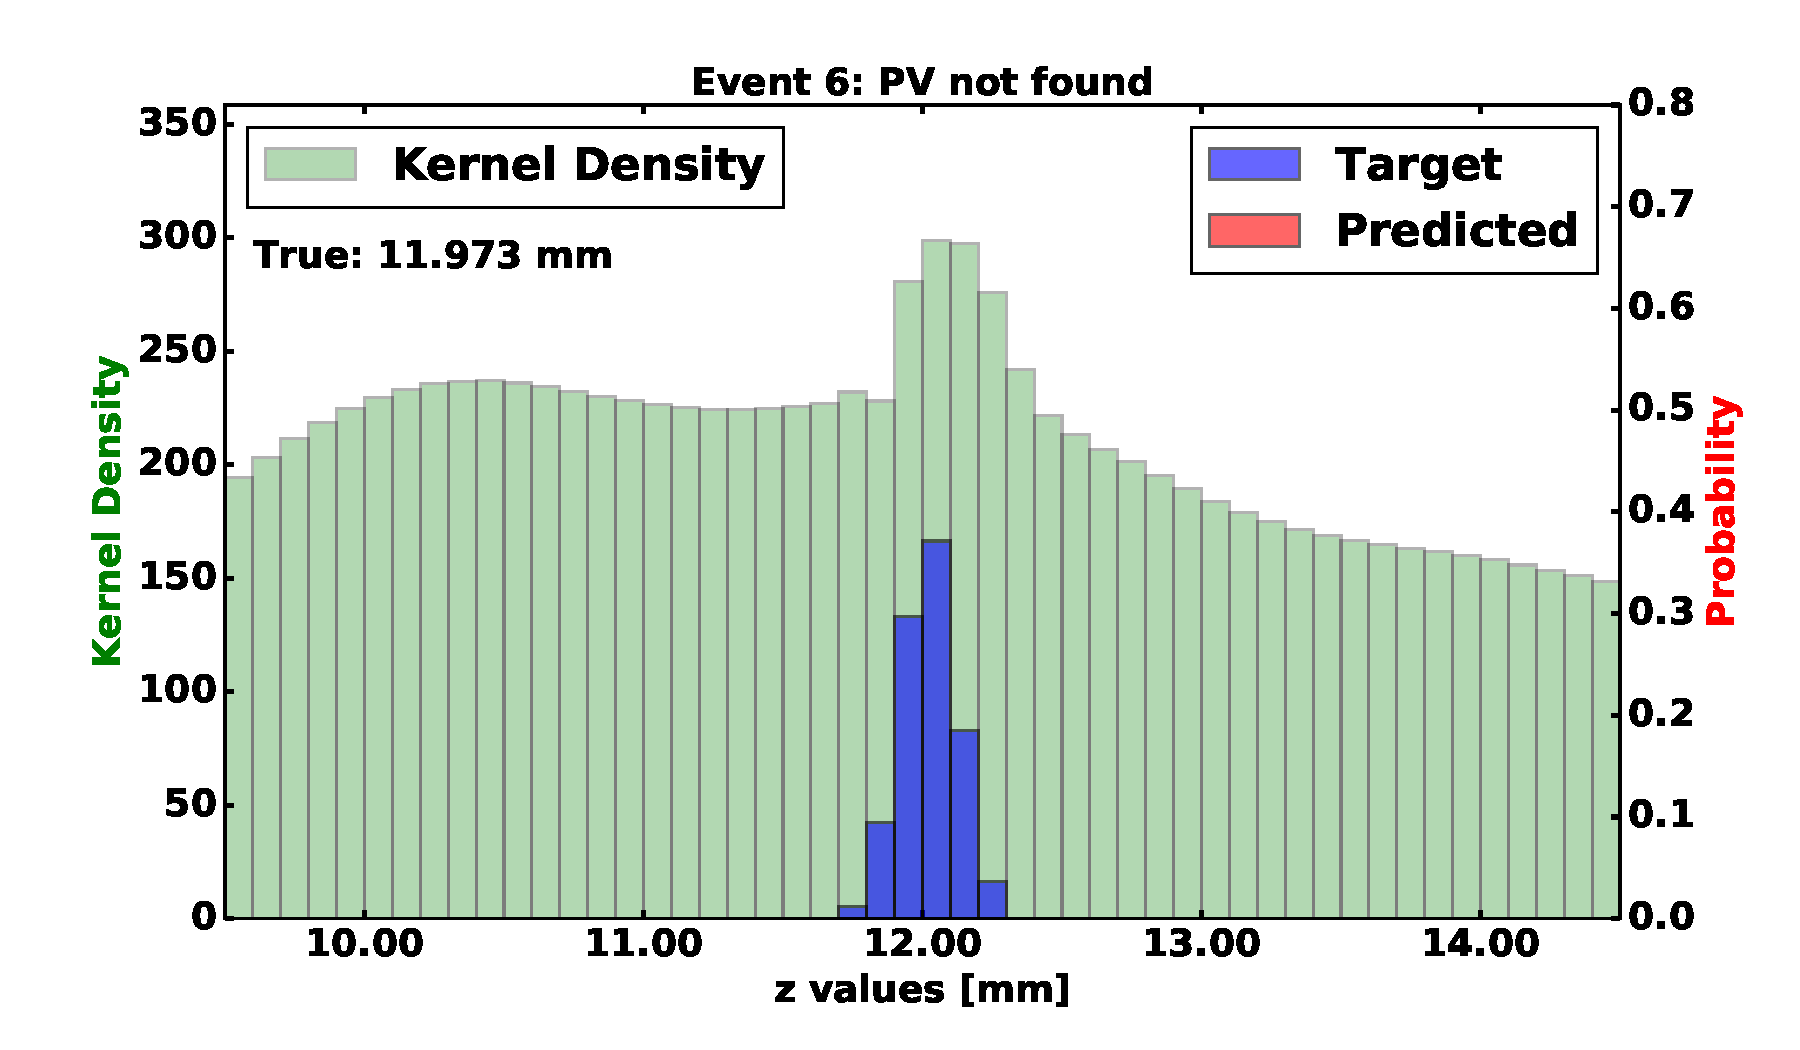
\includegraphics[width=1\textwidth, height=0.45\textwidth,trim=18 0 18 0]{images/120000_3layer_37.pdf}

        \end{center}
    \column{.5\textwidth}
        \begin{center}
           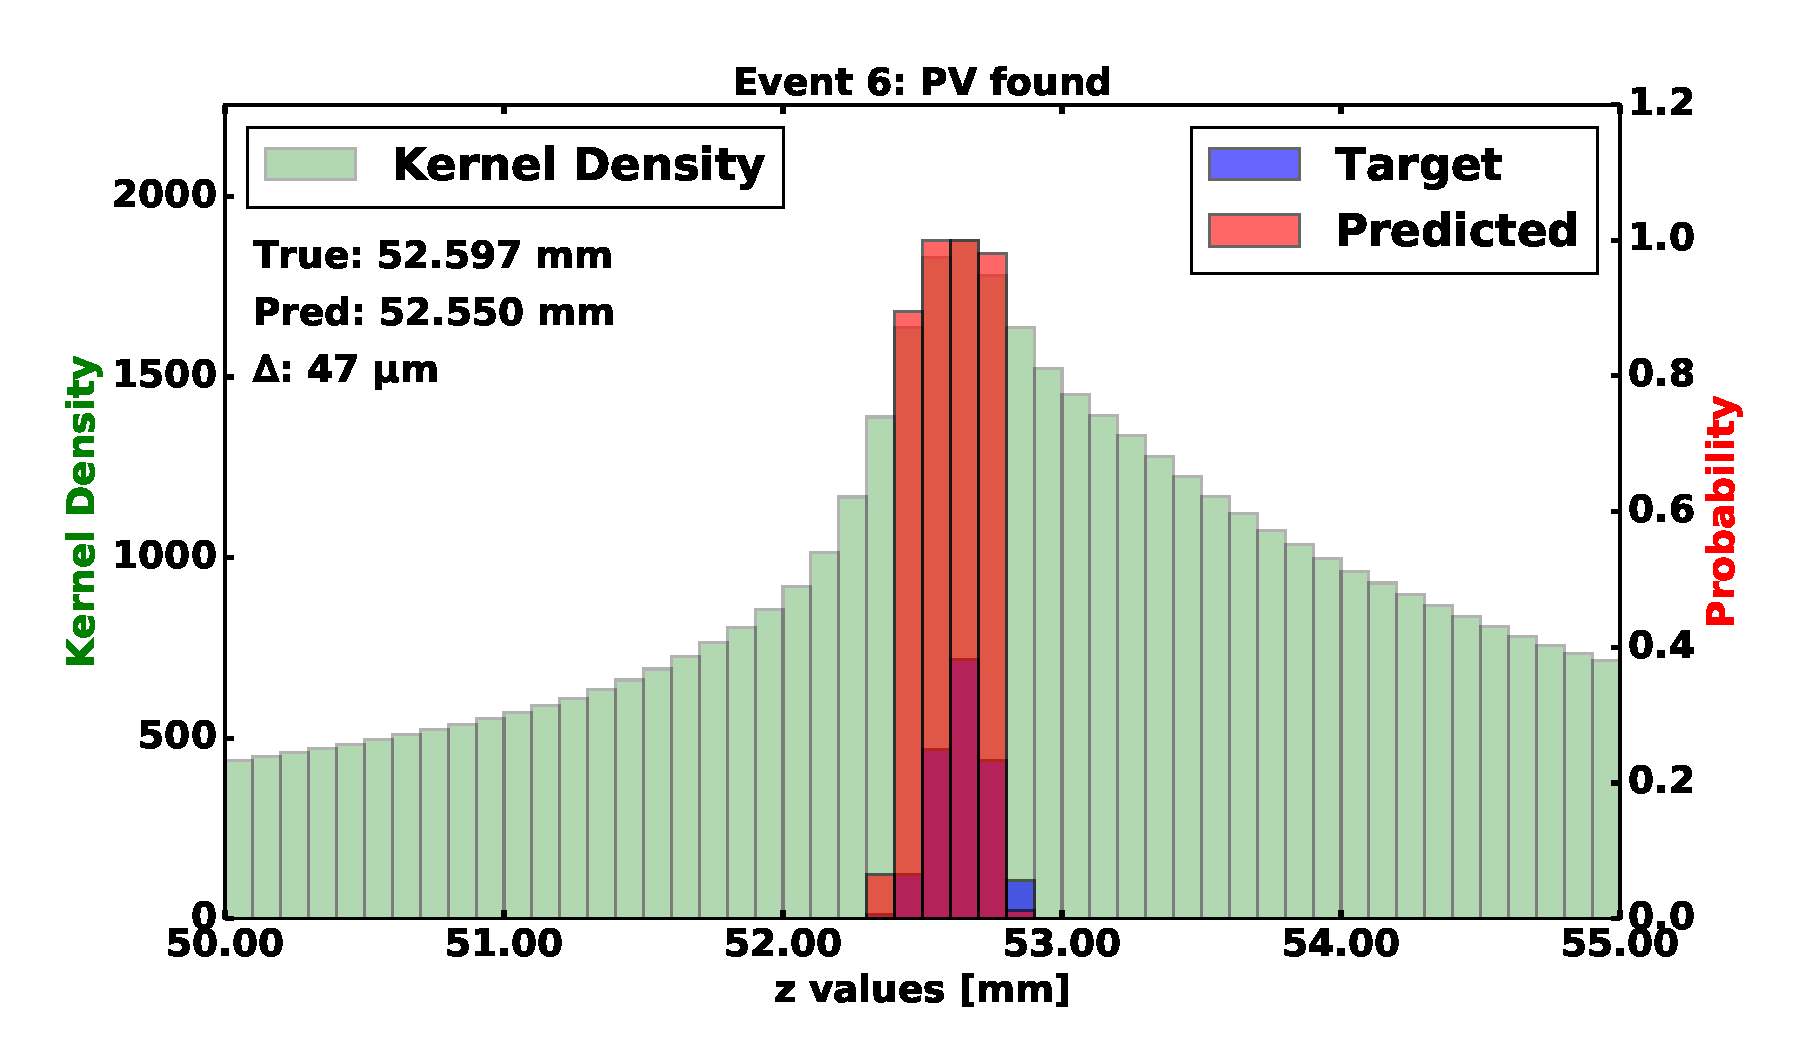
\includegraphics[width=1\textwidth, height=0.45\textwidth, trim=18 0 18 0]{images/120000_3layer_38.pdf}

           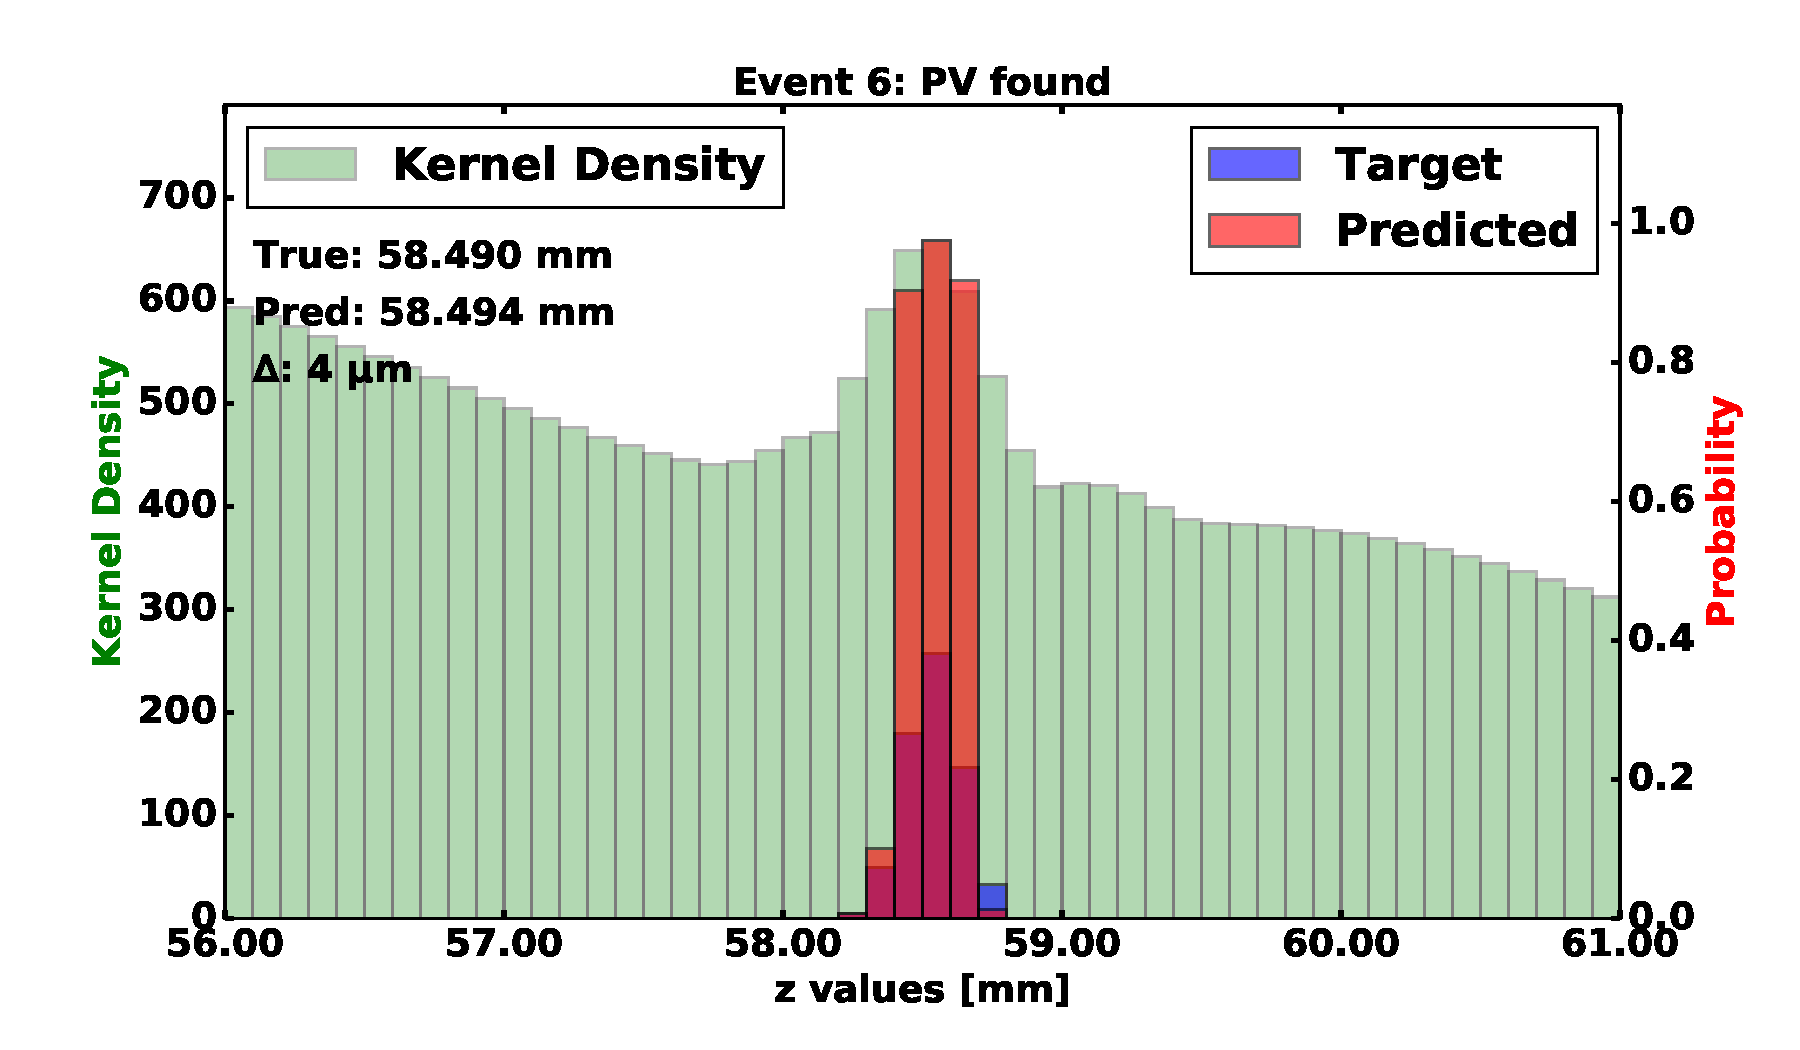
\includegraphics[width=1\textwidth, height=0.45\textwidth, trim=18 0 18 0]{images/120000_3layer_39.pdf}
       \end{center}
  \end{columns}
\end{frame}

\begin{frame}{More Predictions with Targets (3 CVN layers)}
  \begin{columns}[c]
    \column{.5\textwidth}
        \begin{center}
            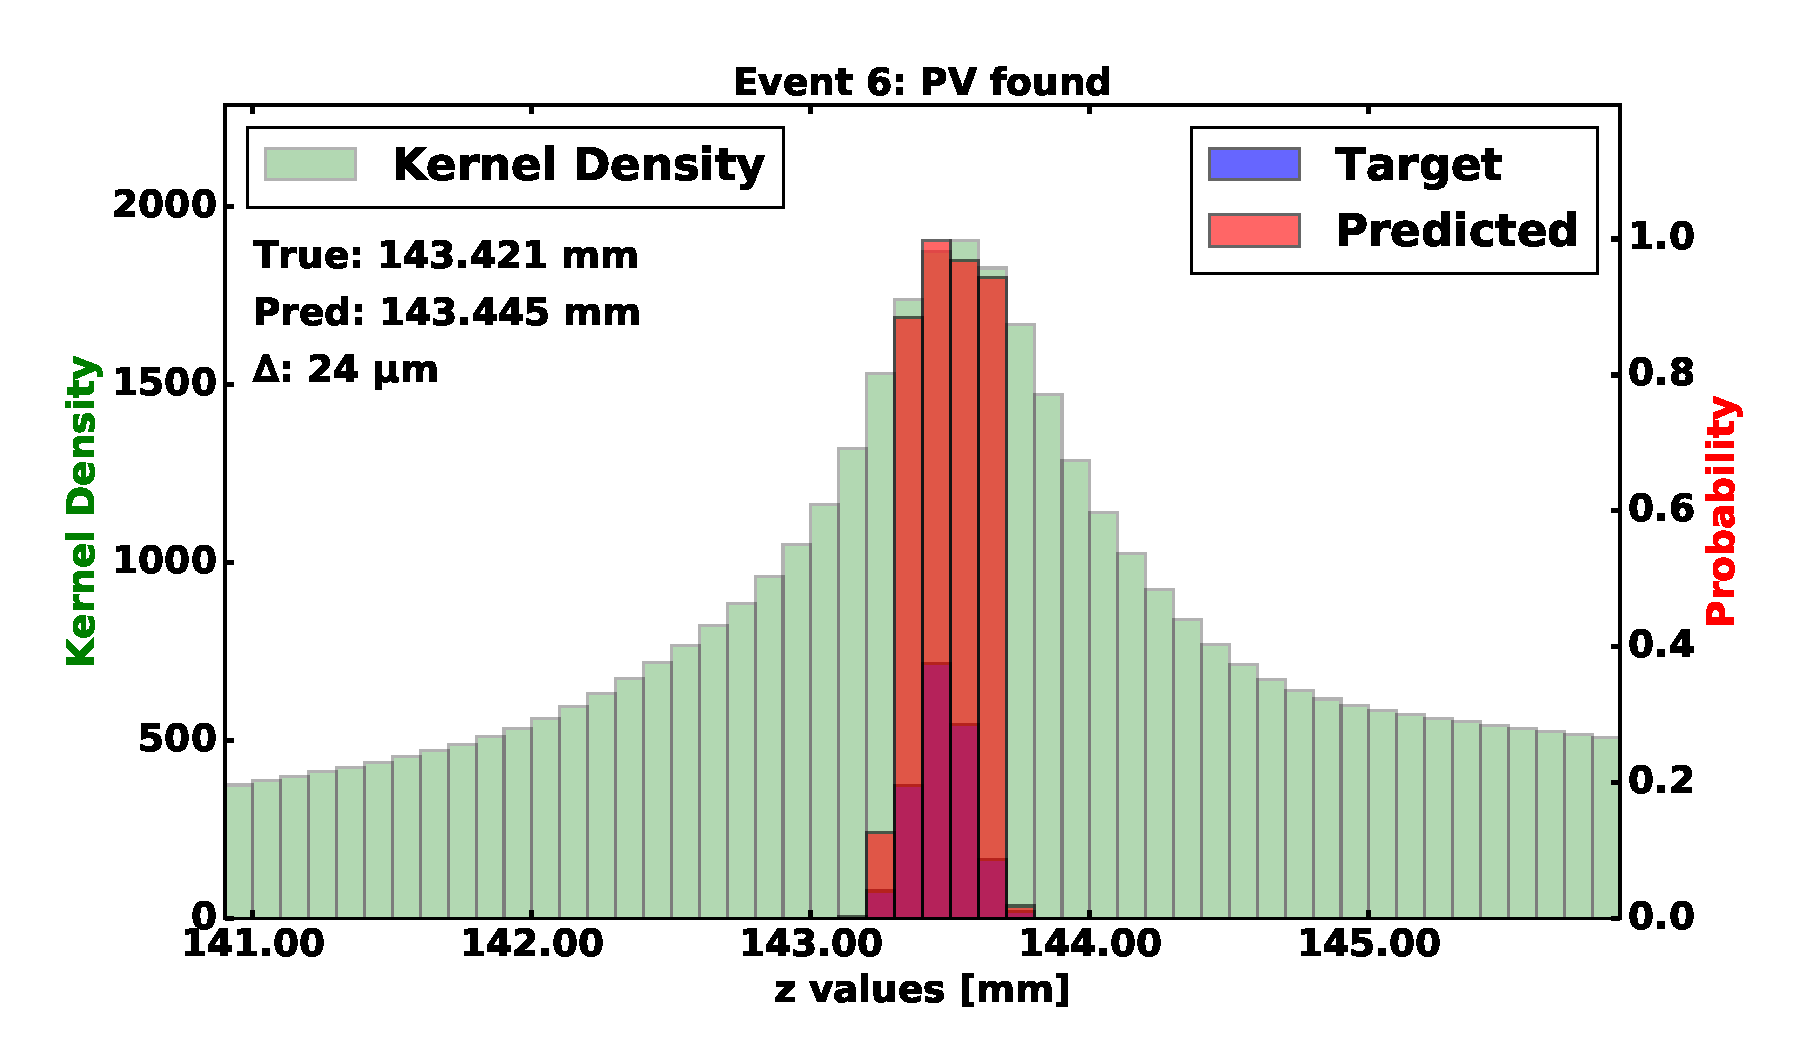
\includegraphics[width=1\textwidth,height=0.45\textwidth, trim=18 0 18 0]{images/120000_3layer_40.pdf}

            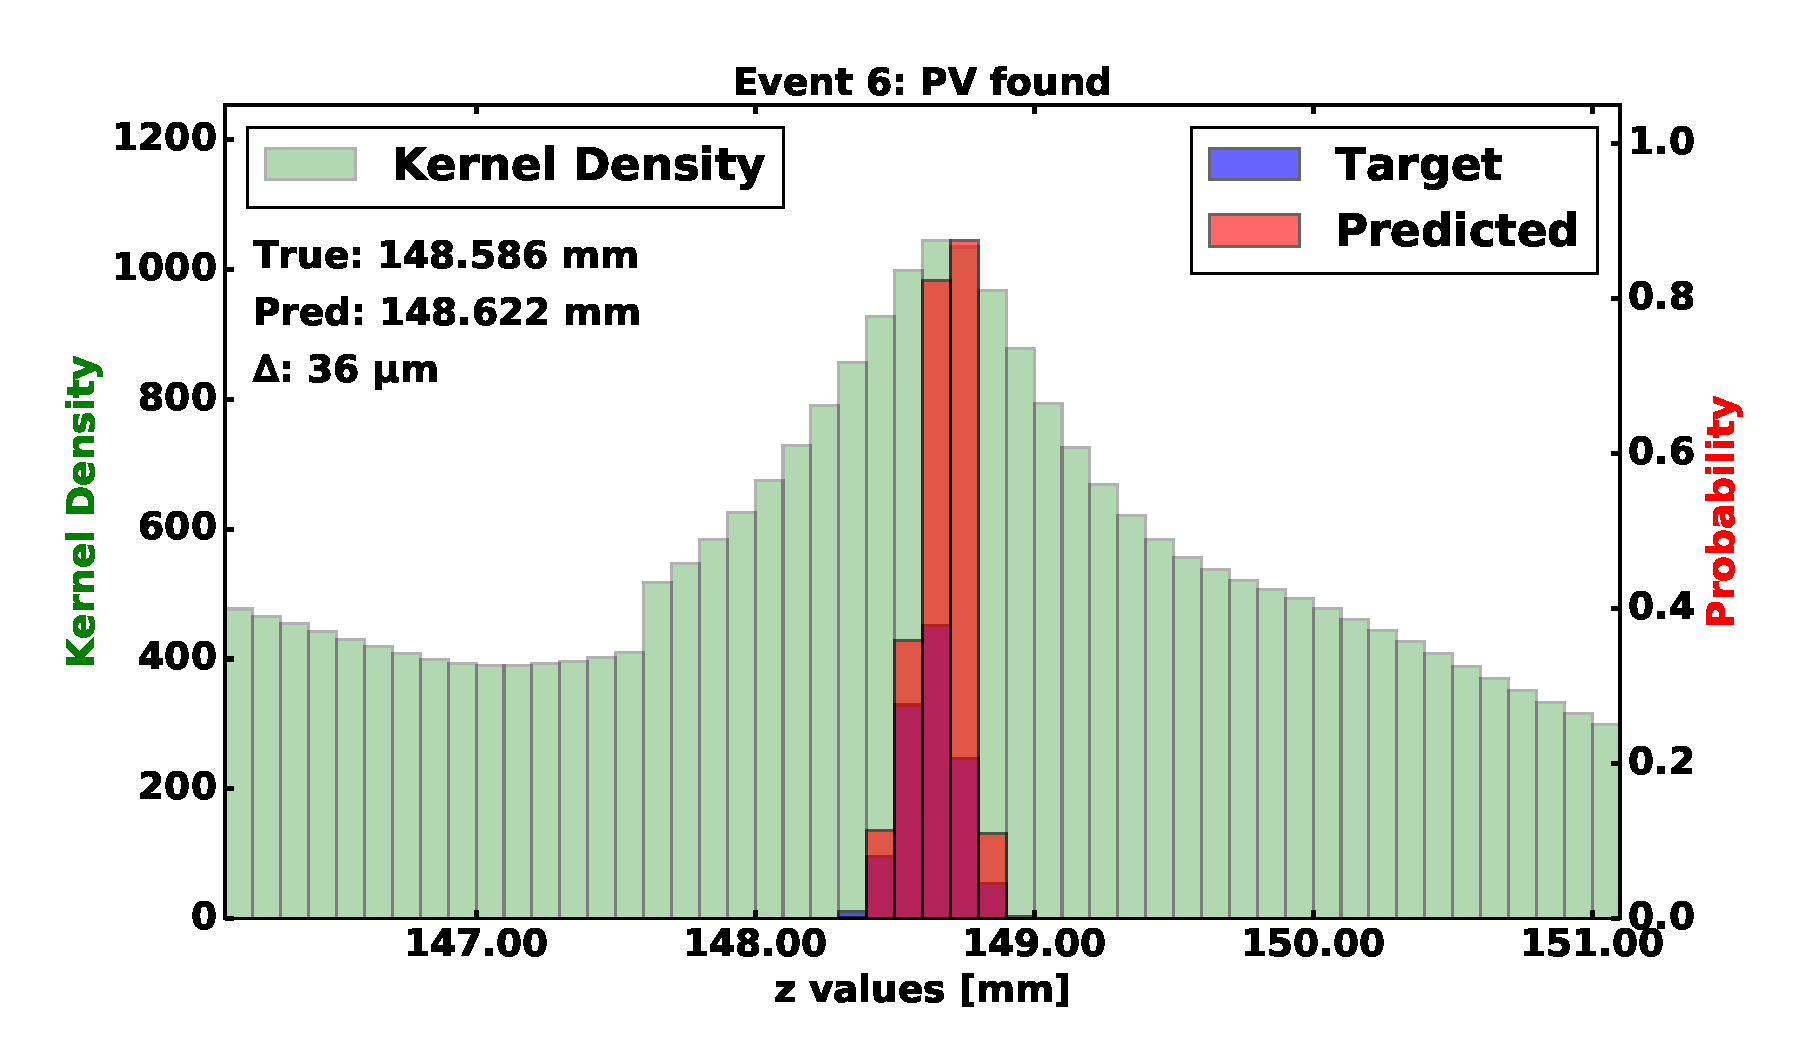
\includegraphics[width=1\textwidth, height=0.45\textwidth,trim=18 0 18 0]{images/120000_3layer_41.pdf}

        \end{center}
    \column{.5\textwidth}
        \begin{center}
           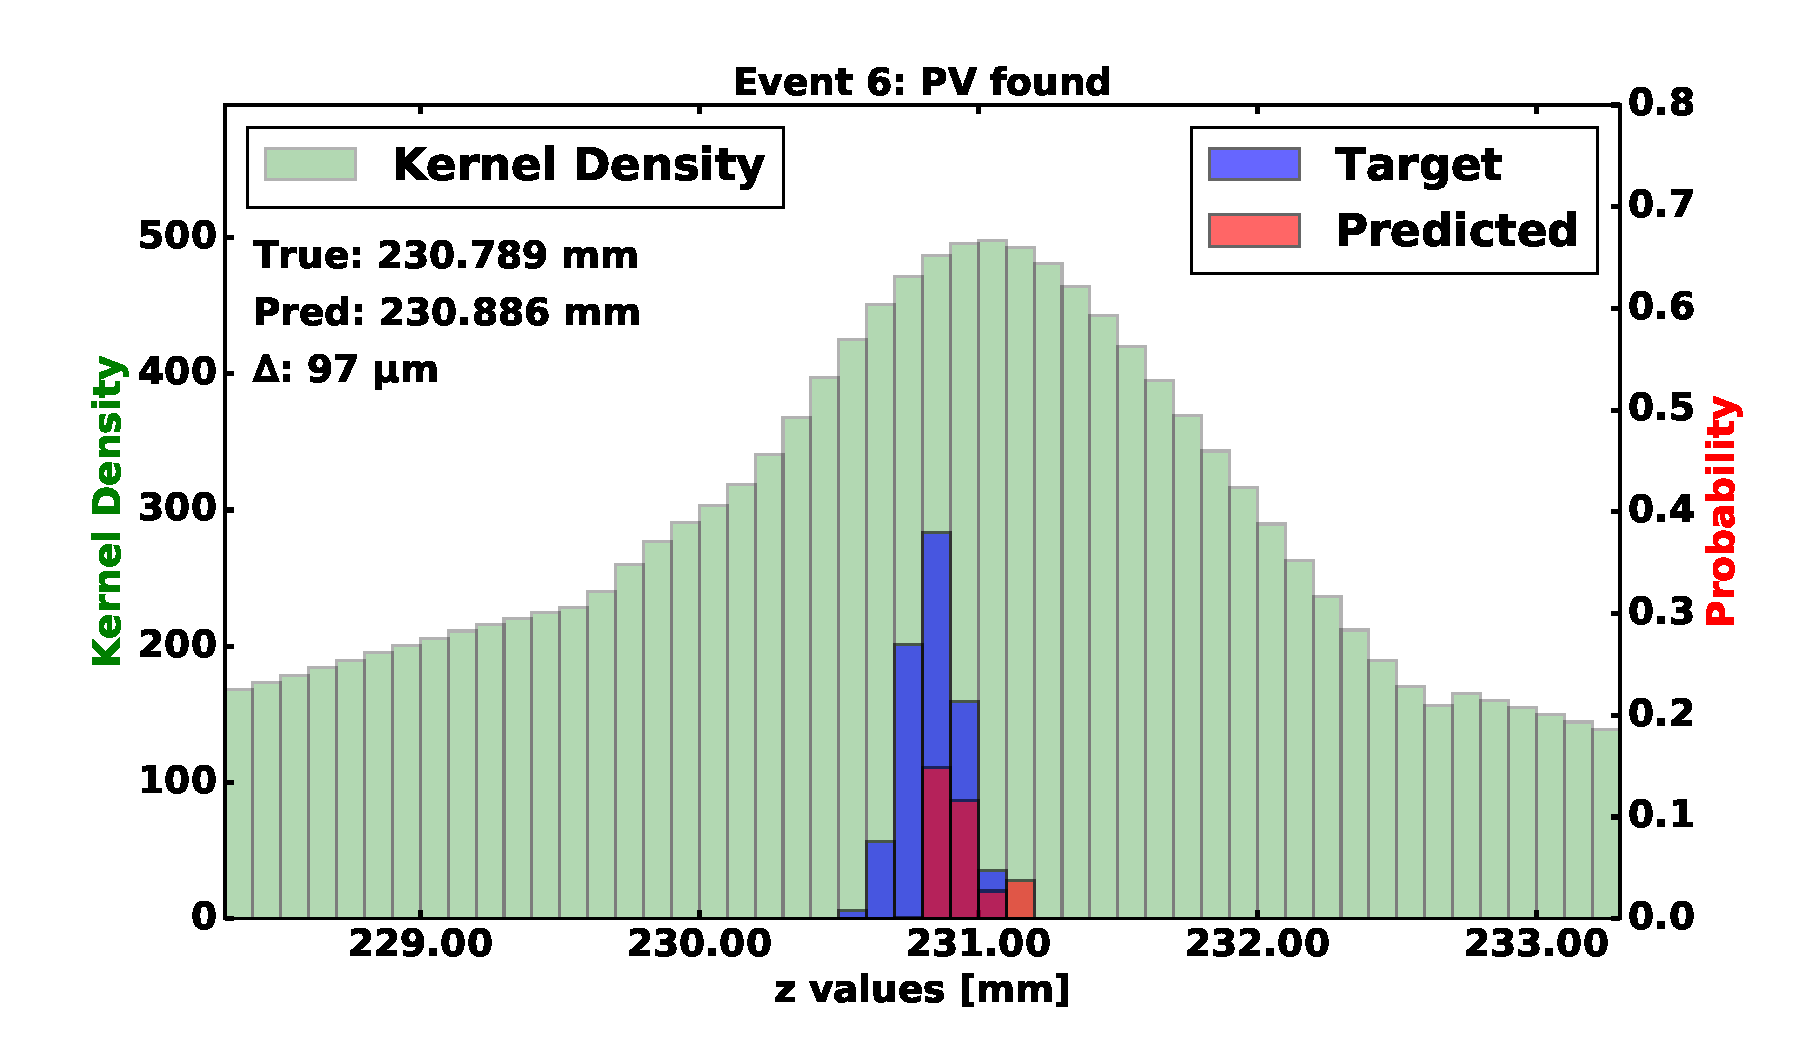
\includegraphics[width=1\textwidth, height=0.45\textwidth, trim=18 0 18 0]{images/120000_3layer_42.pdf}

           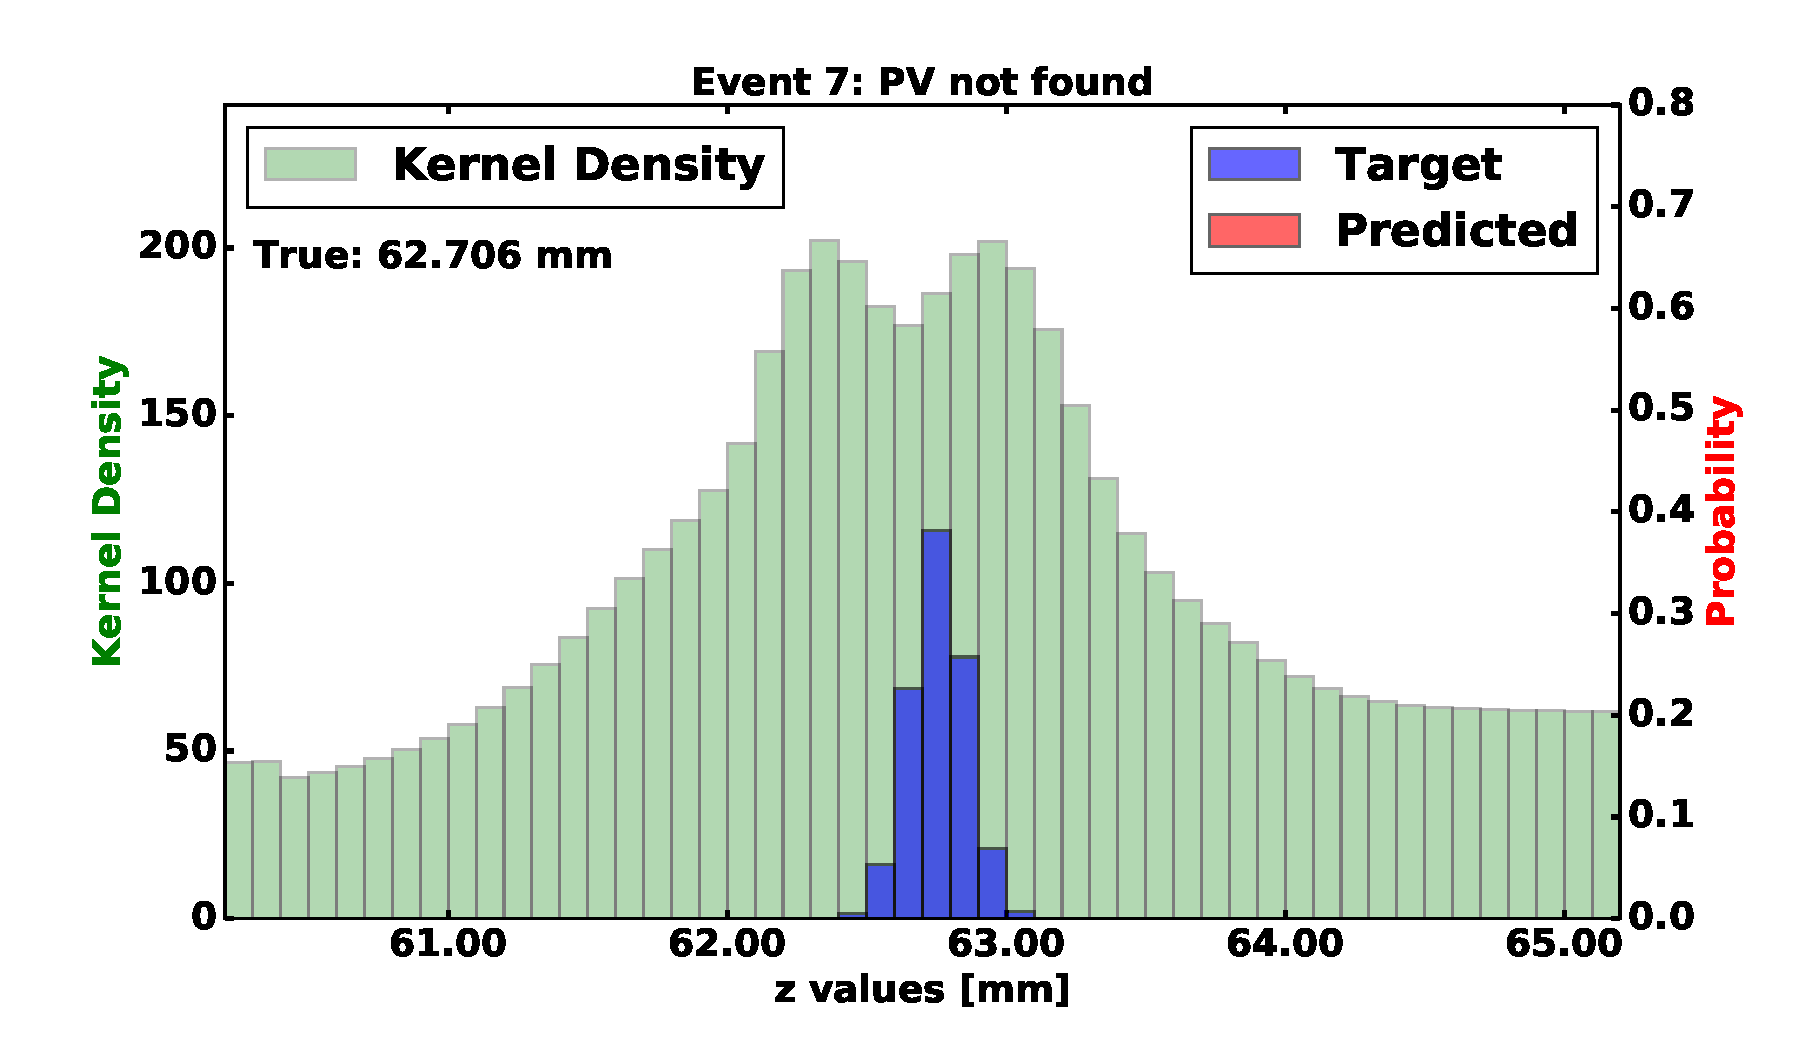
\includegraphics[width=1\textwidth, height=0.45\textwidth, trim=18 0 18 0]{images/120000_3layer_43.pdf}
       \end{center}
  \end{columns}
\end{frame}

\begin{frame}{More Predictions with Targets (3 CVN layers)}
  \begin{columns}[c]
    \column{.5\textwidth}
        \begin{center}
            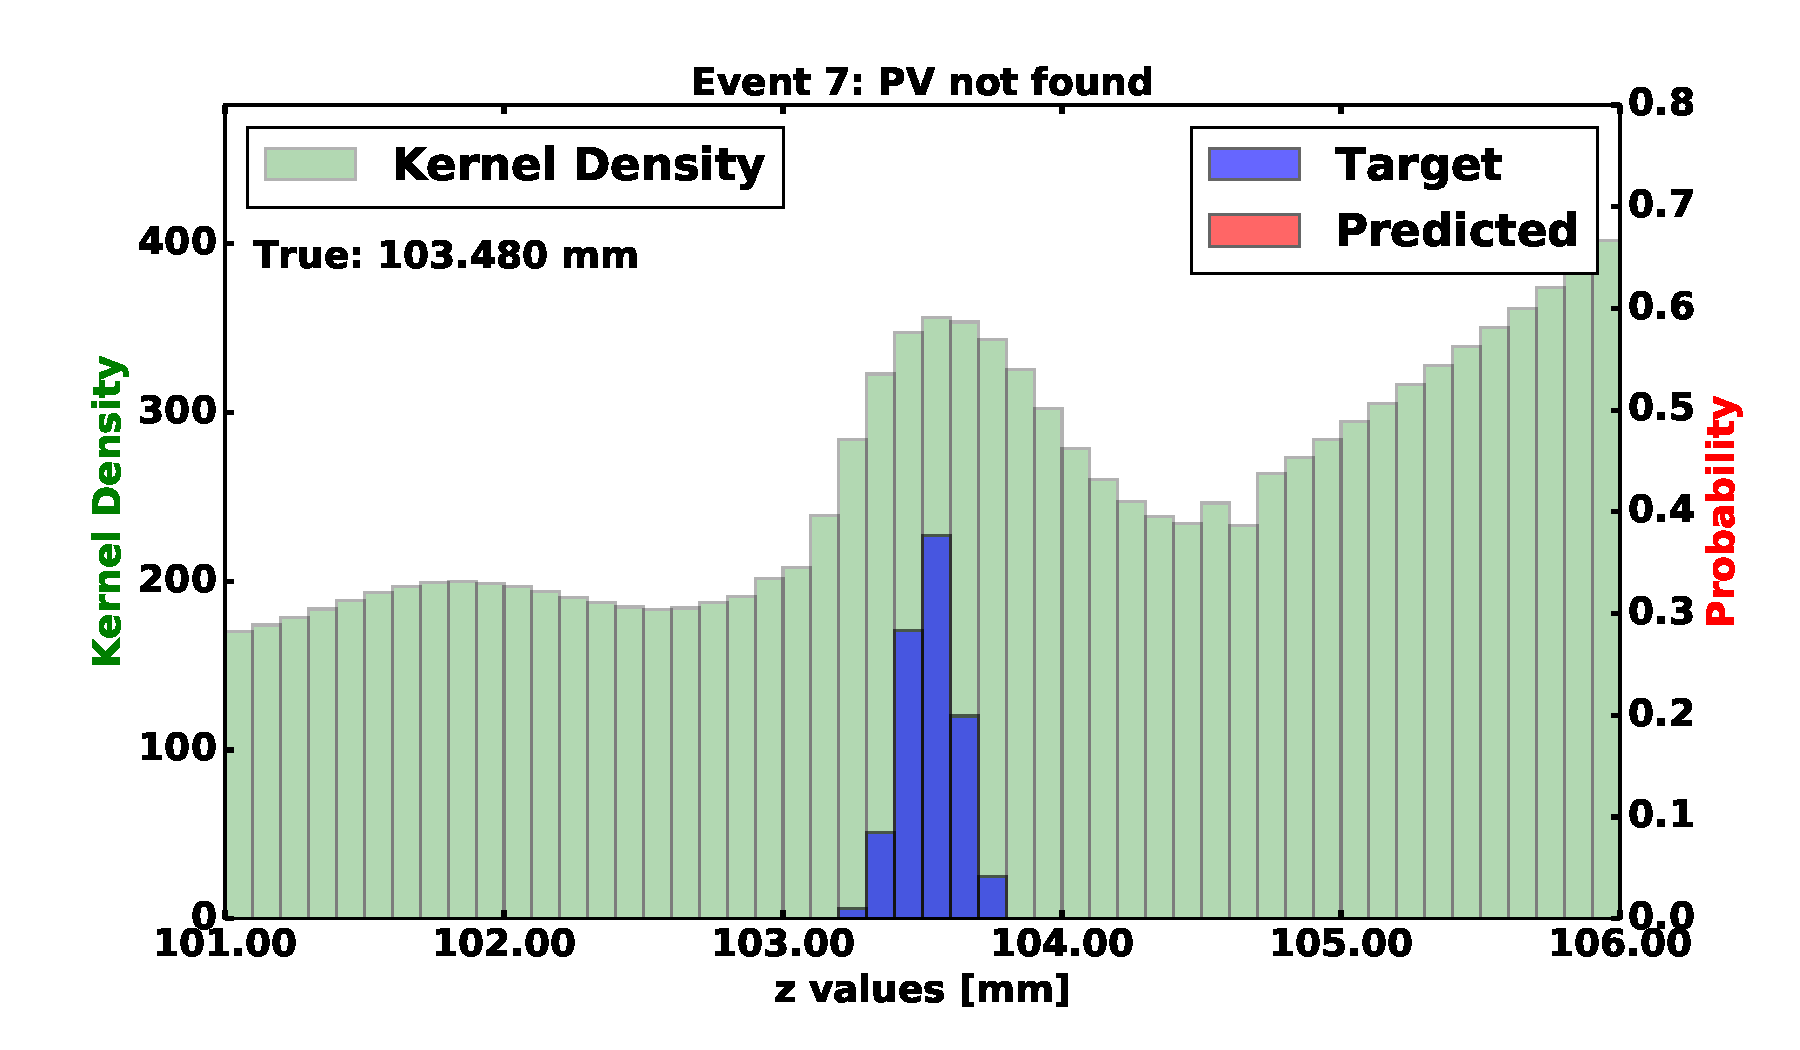
\includegraphics[width=1\textwidth,height=0.45\textwidth, trim=18 0 18 0]{images/120000_3layer_45.pdf}

            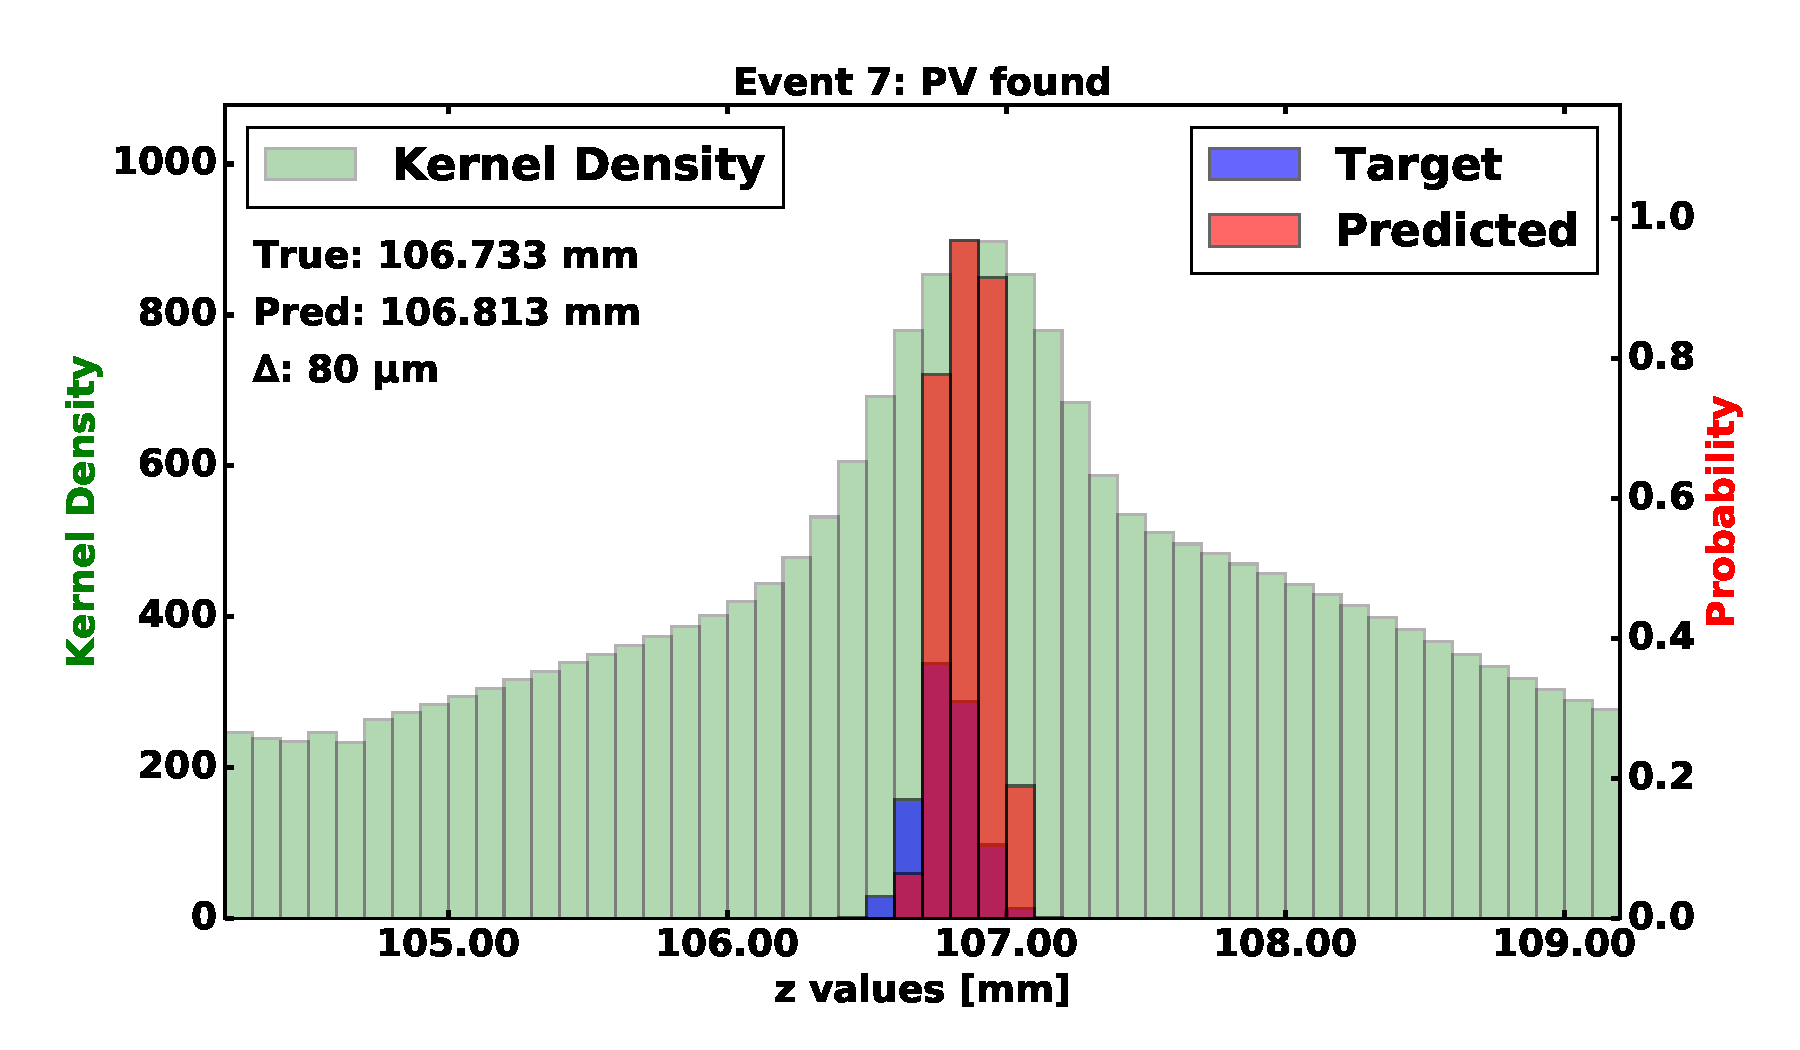
\includegraphics[width=1\textwidth, height=0.45\textwidth,trim=18 0 18 0]{images/120000_3layer_46.pdf}

        \end{center}
    \column{.5\textwidth}
        \begin{center}
           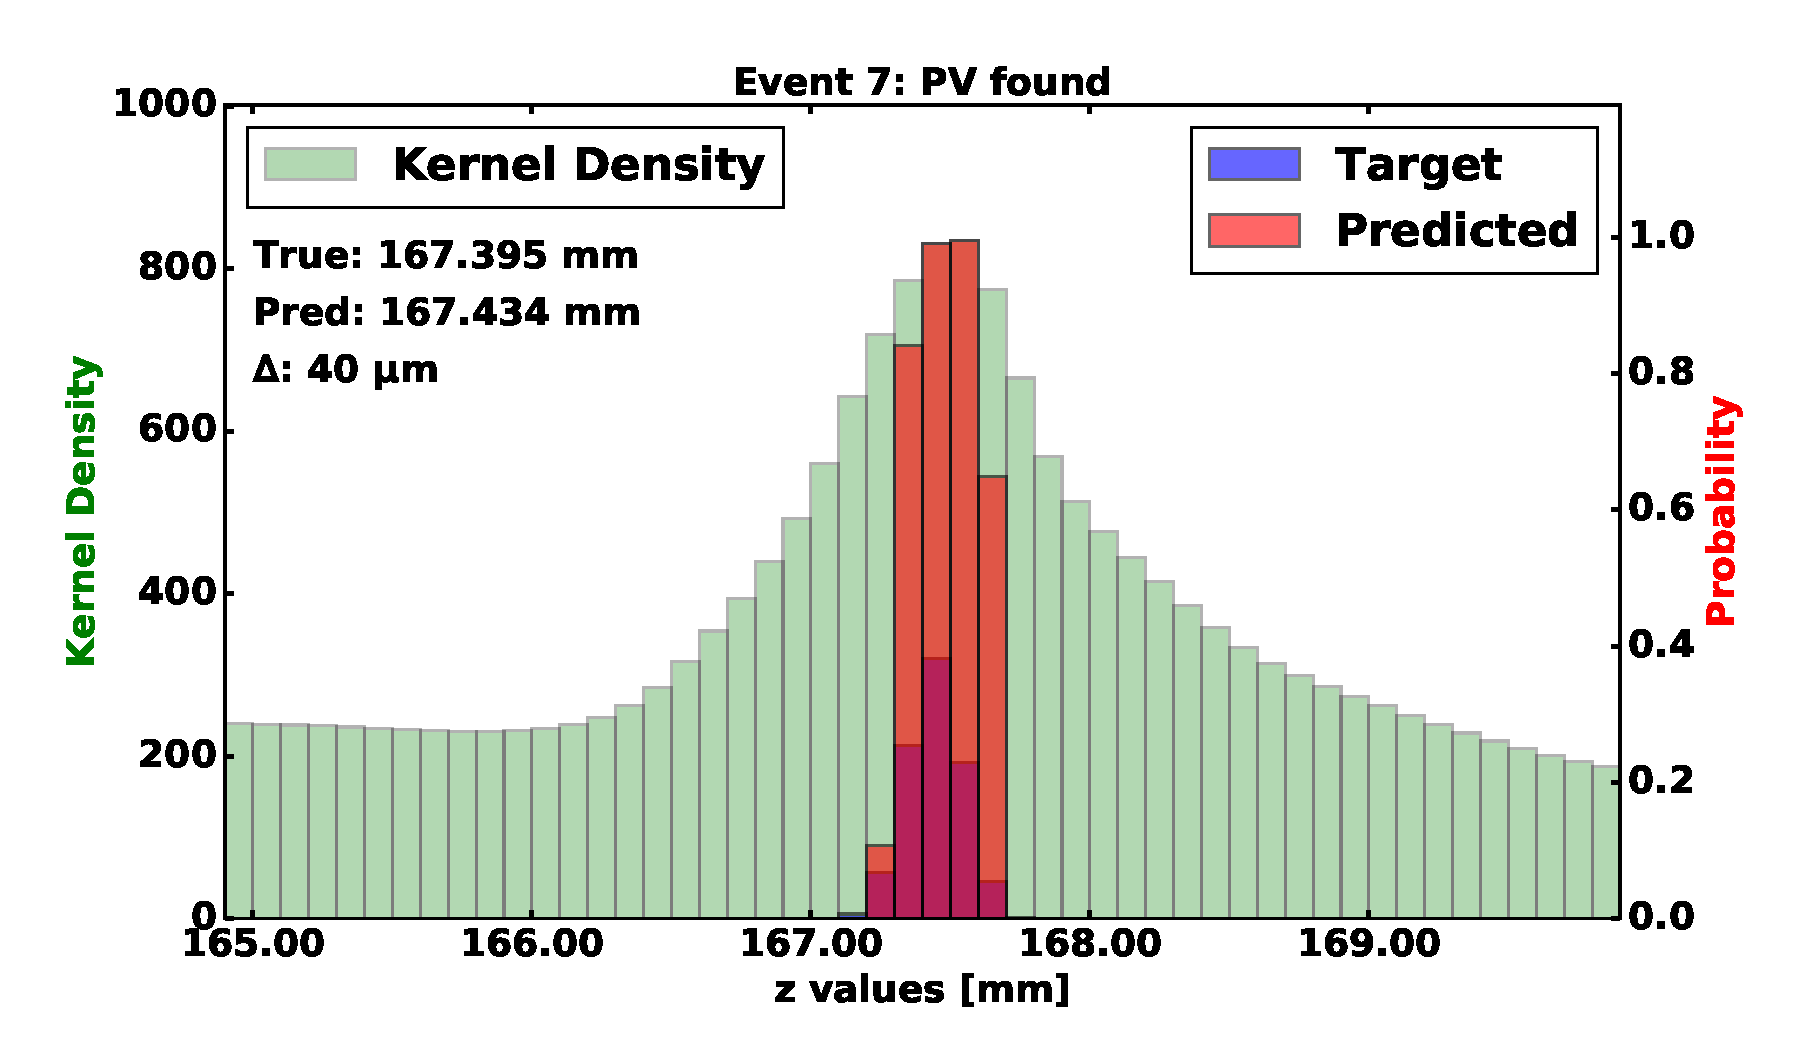
\includegraphics[width=1\textwidth, height=0.45\textwidth, trim=18 0 18 0]{images/120000_3layer_47.pdf}

           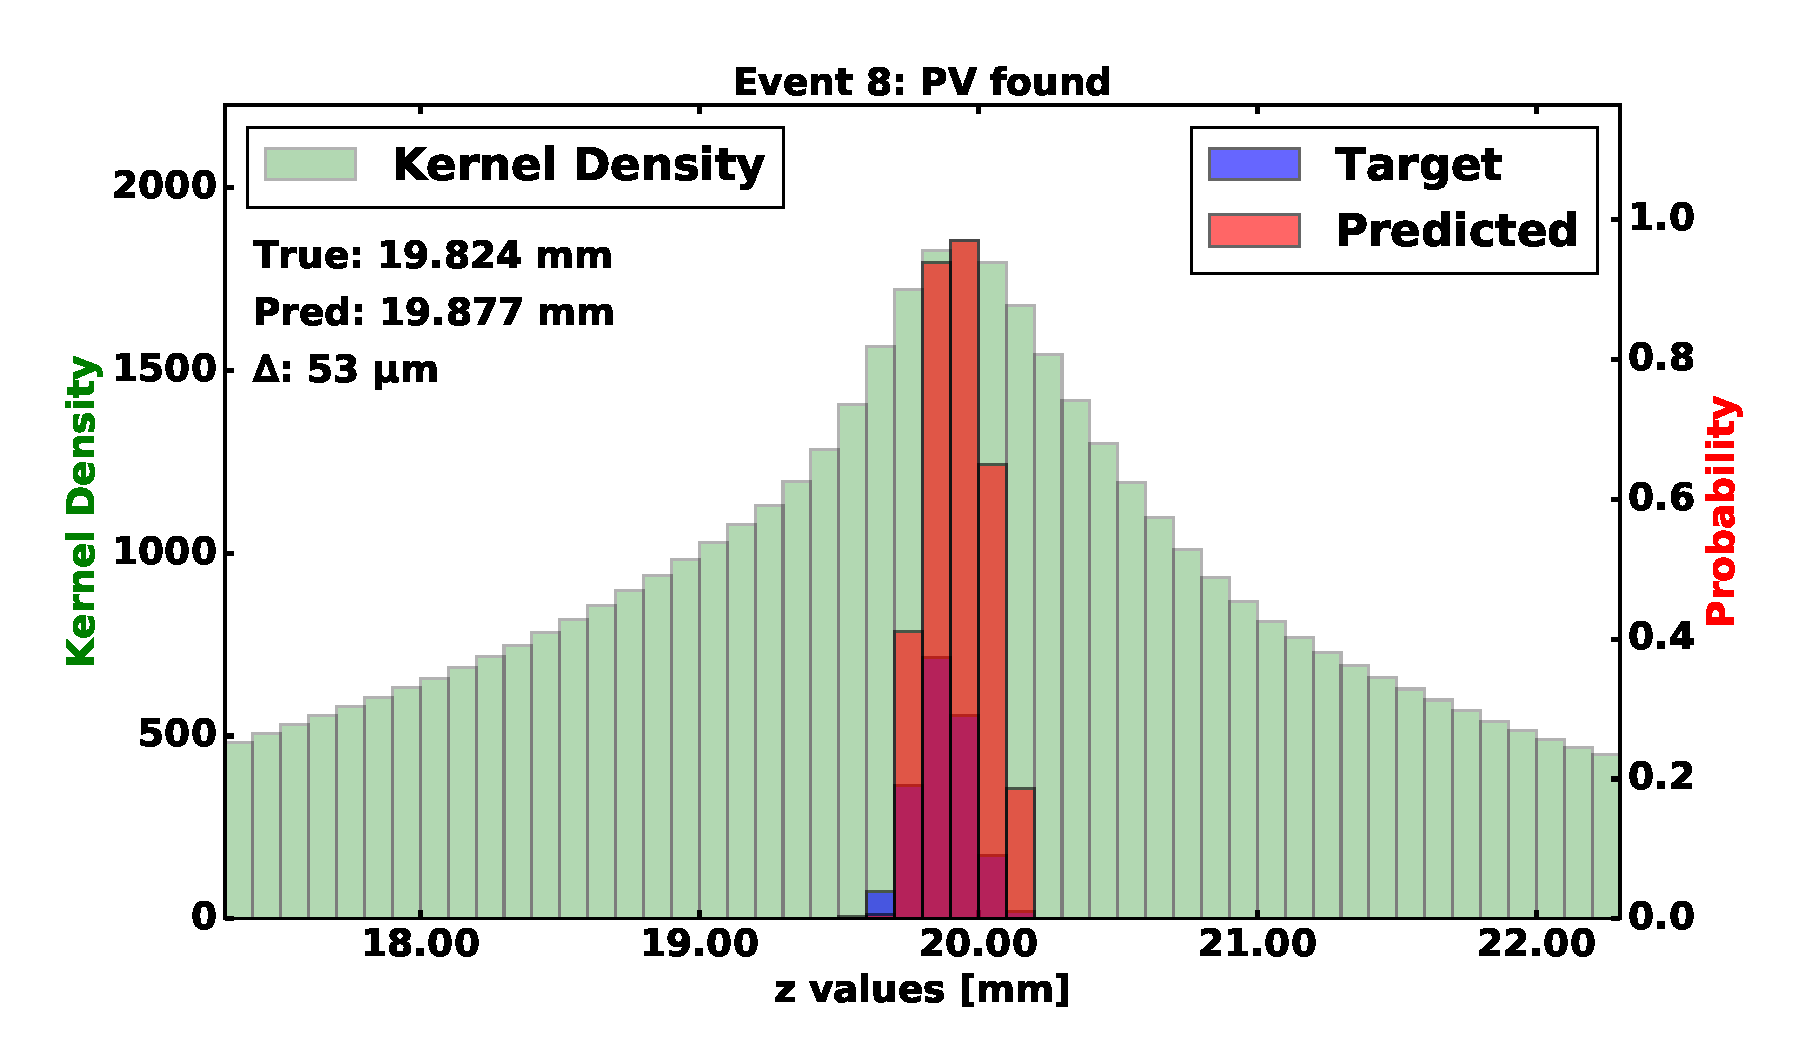
\includegraphics[width=1\textwidth, height=0.45\textwidth, trim=18 0 18 0]{images/120000_3layer_48.pdf}
       \end{center}
  \end{columns}
\end{frame}

\begin{frame}{More Predictions with Targets (3 CVN layers)}
  \begin{columns}[c]
    \column{.5\textwidth}
        \begin{center}
            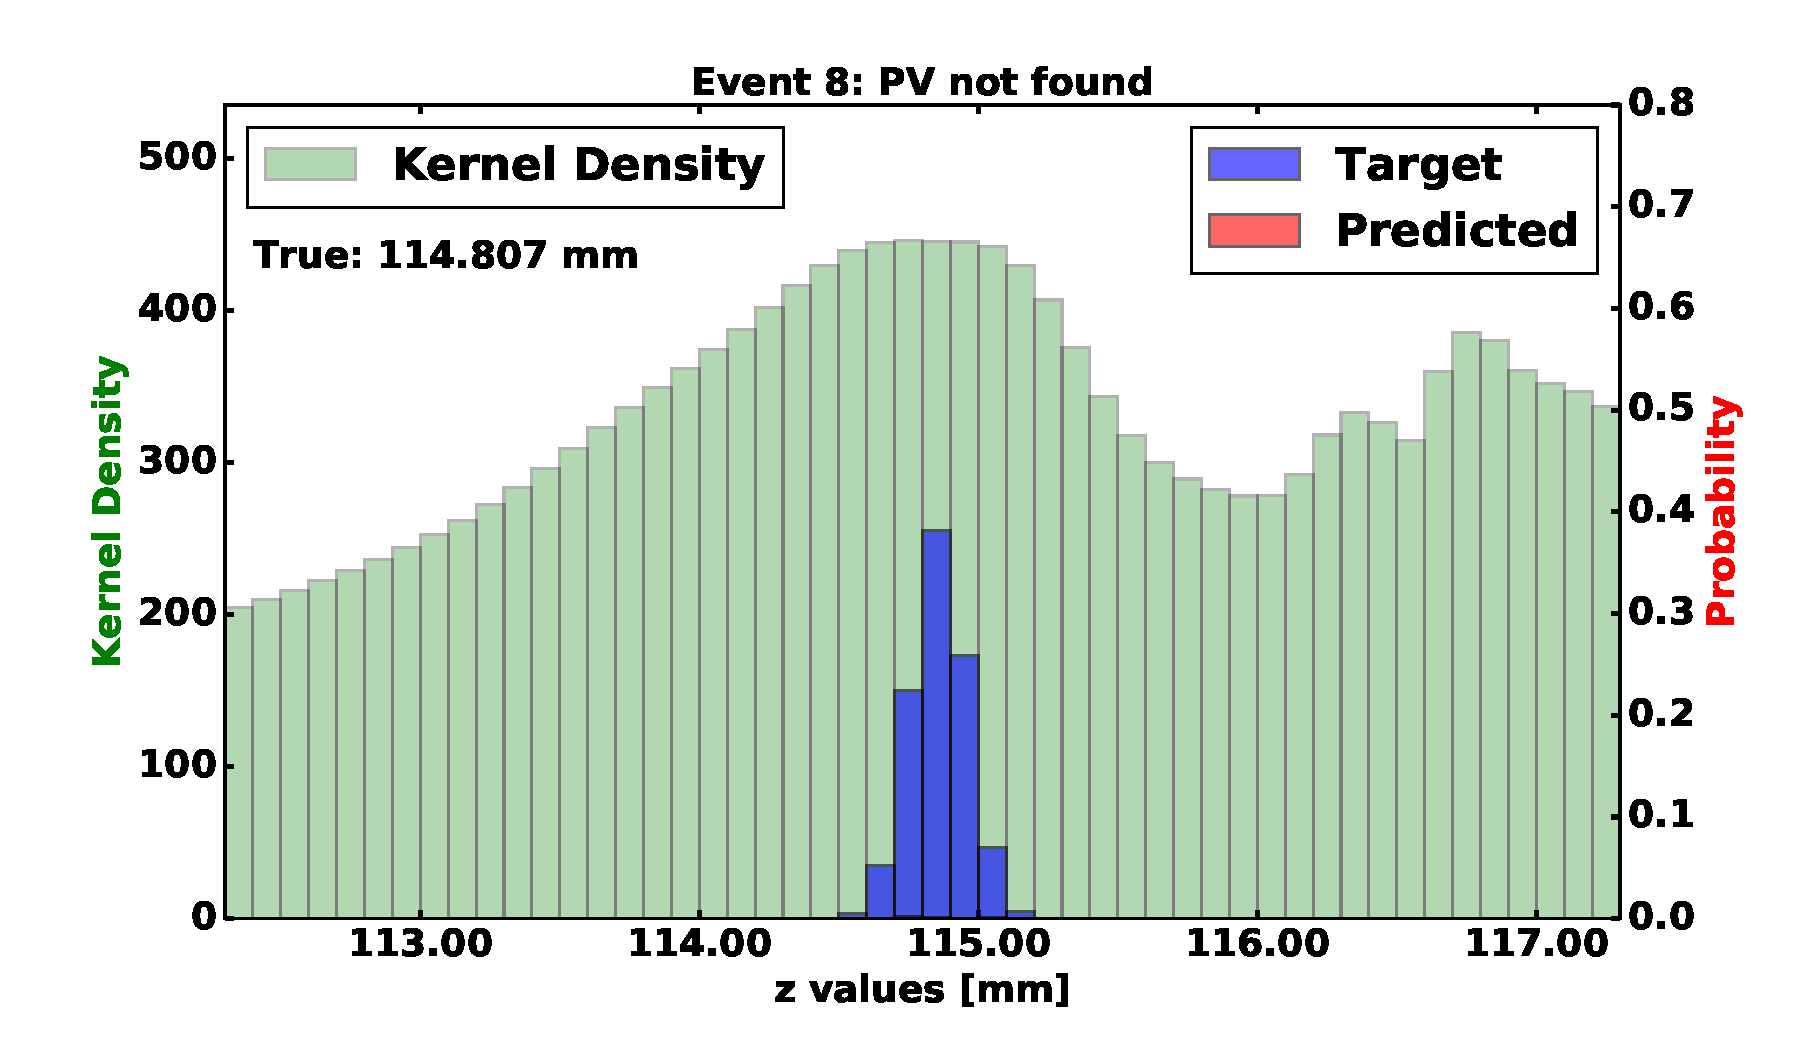
\includegraphics[width=1\textwidth,height=0.45\textwidth, trim=18 0 18 0]{images/120000_3layer_49.pdf}

            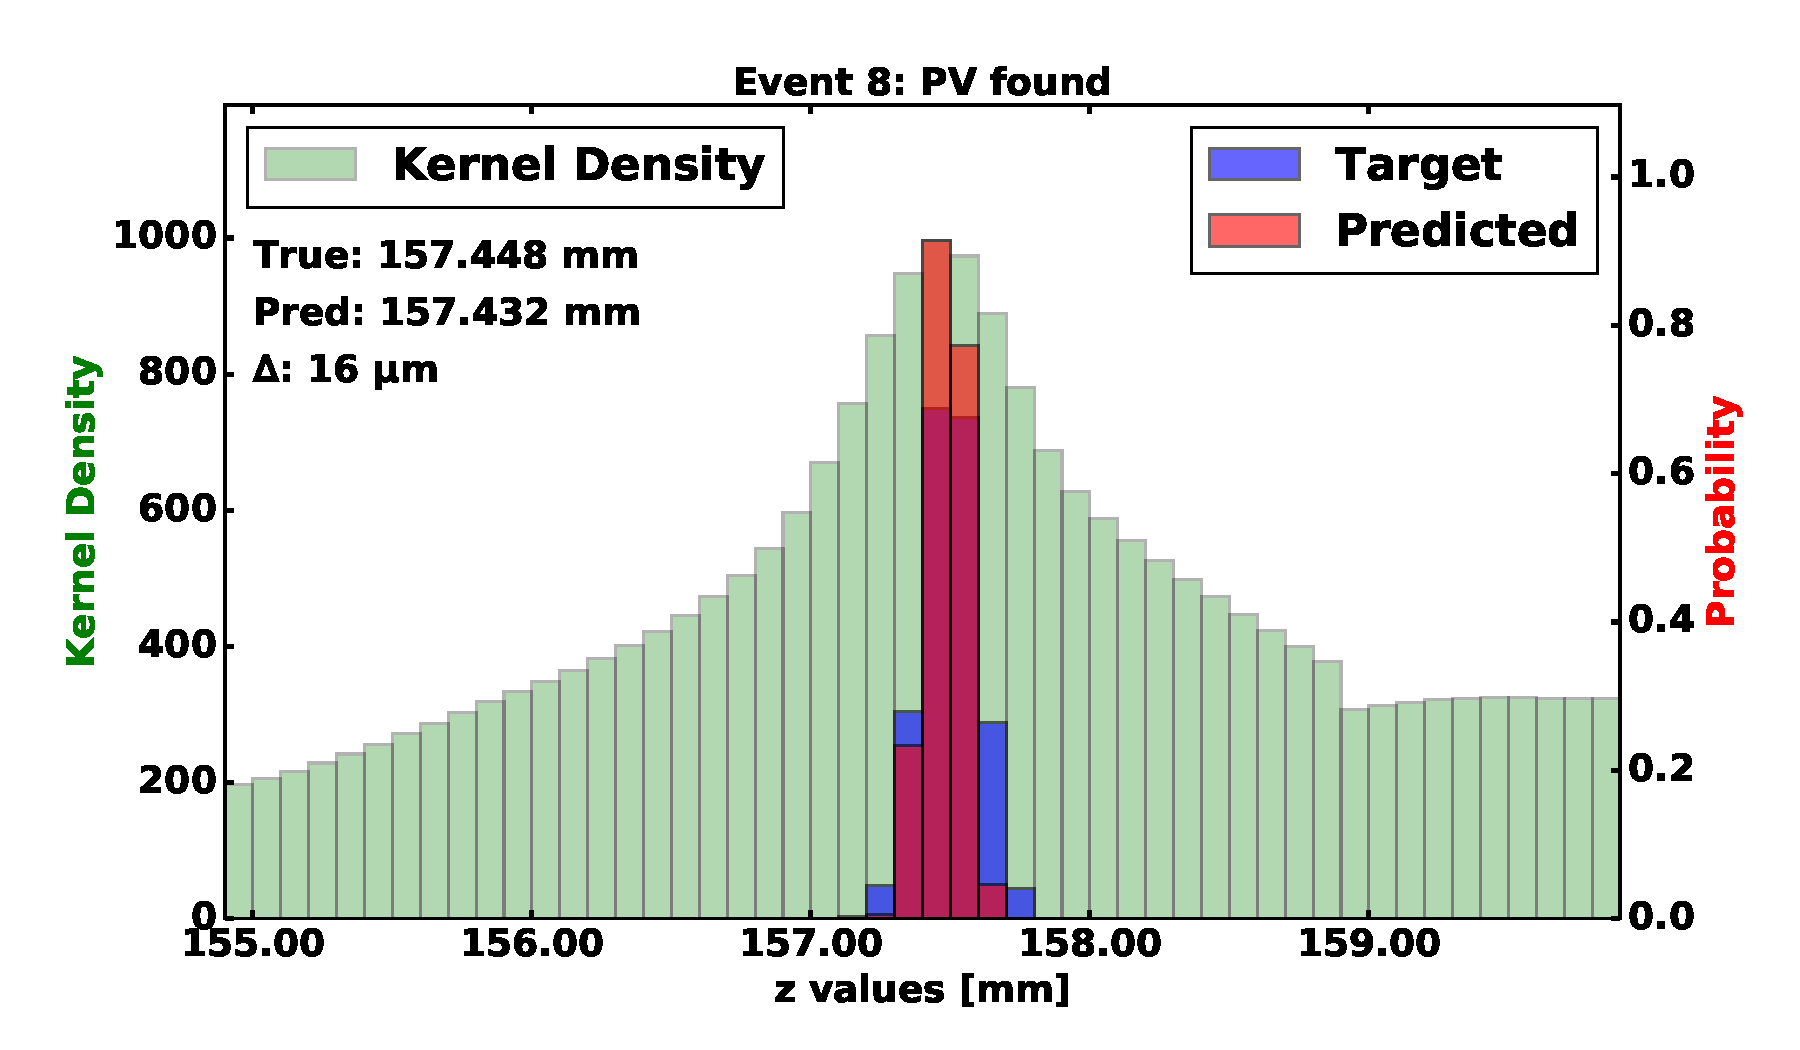
\includegraphics[width=1\textwidth, height=0.45\textwidth,trim=18 0 18 0]{images/120000_3layer_50.pdf}

        \end{center}
    \column{.5\textwidth}
        \begin{center}
           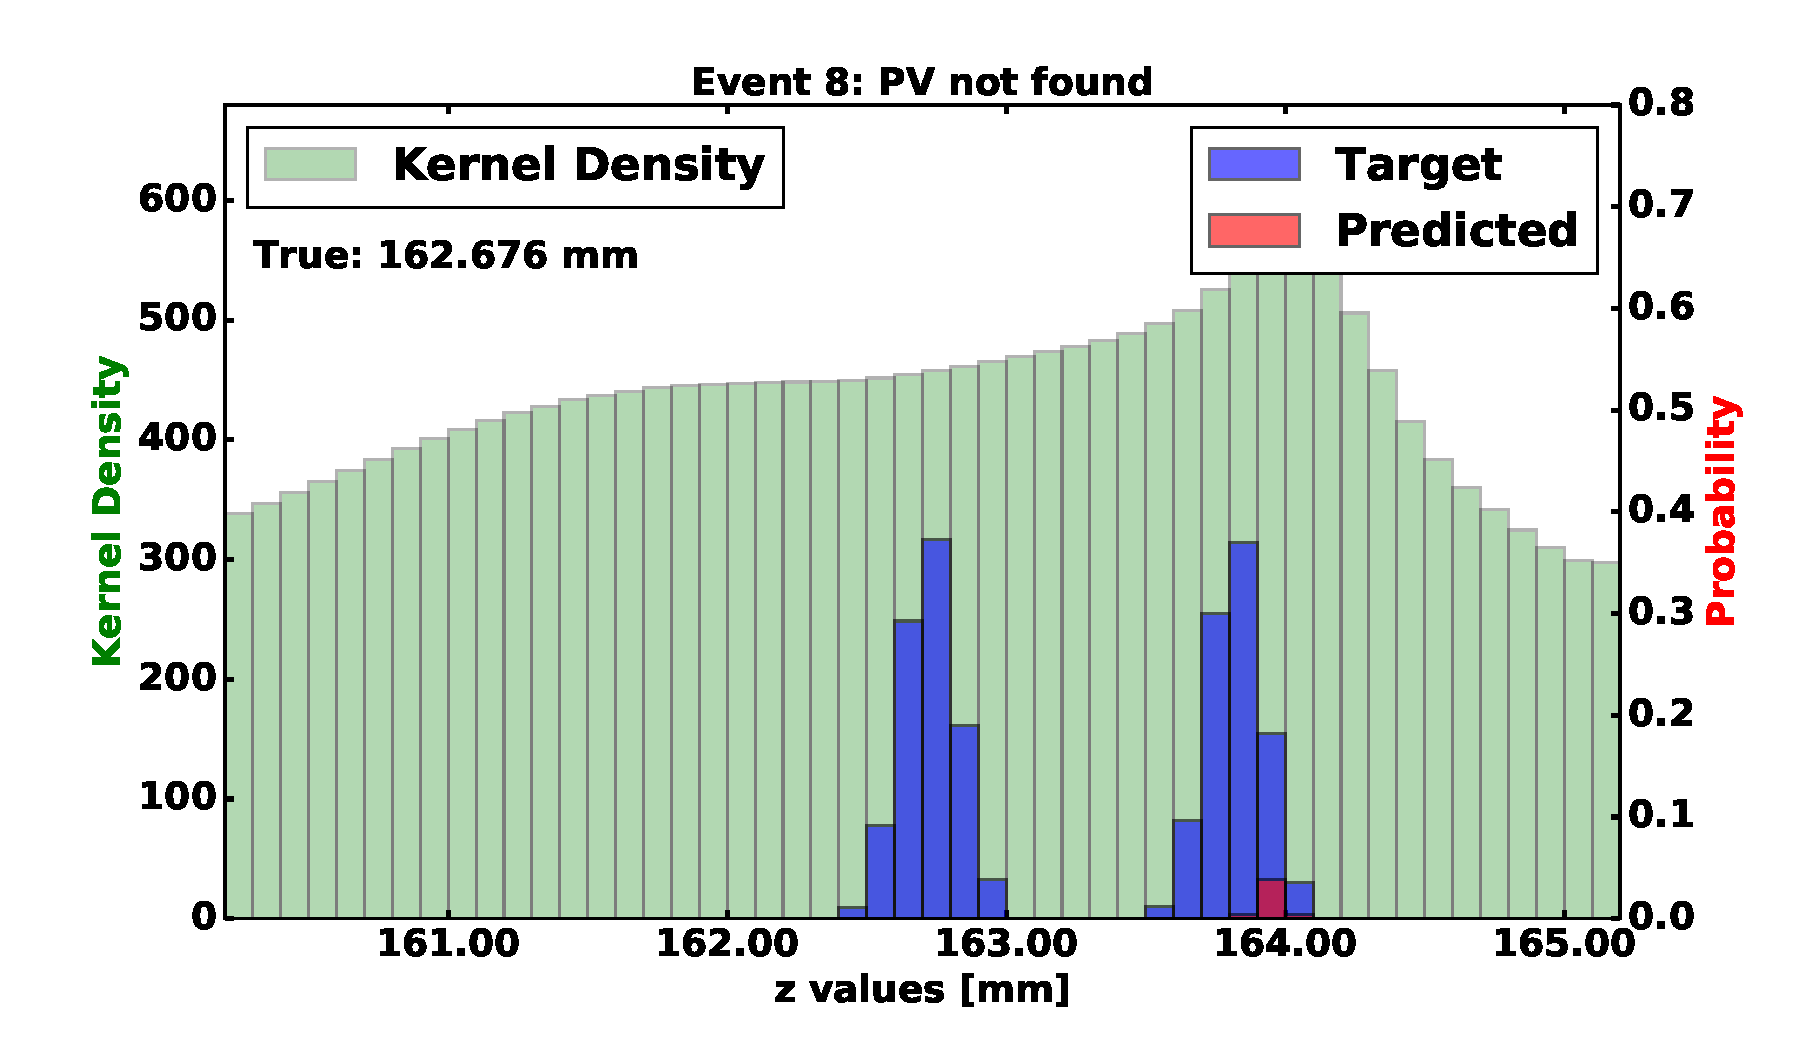
\includegraphics[width=1\textwidth, height=0.45\textwidth, trim=18 0 18 0]{images/120000_3layer_51.pdf}

           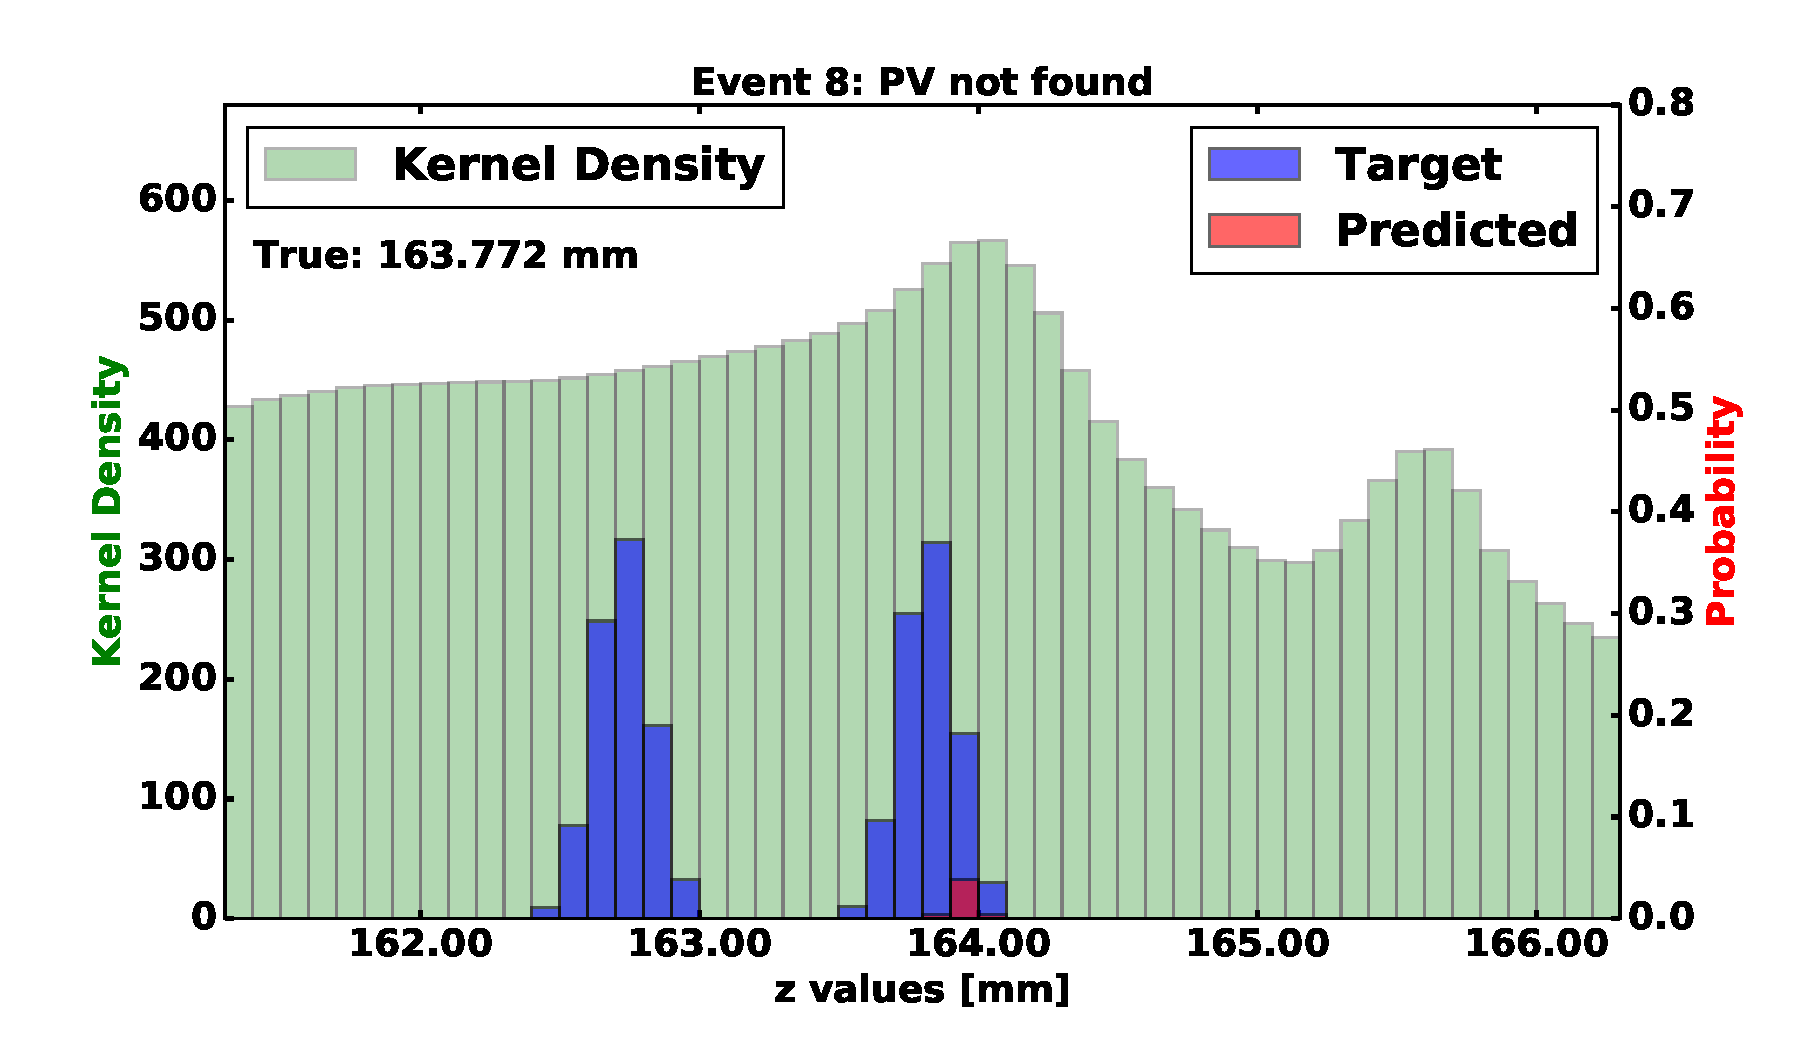
\includegraphics[width=1\textwidth, height=0.45\textwidth, trim=18 0 18 0]{images/120000_3layer_52.pdf}
       \end{center}
  \end{columns}
\end{frame}

\begin{frame}{More Predictions with Targets (3 CVN layers)}
  \begin{columns}[c]
    \column{.5\textwidth}
        \begin{center}
            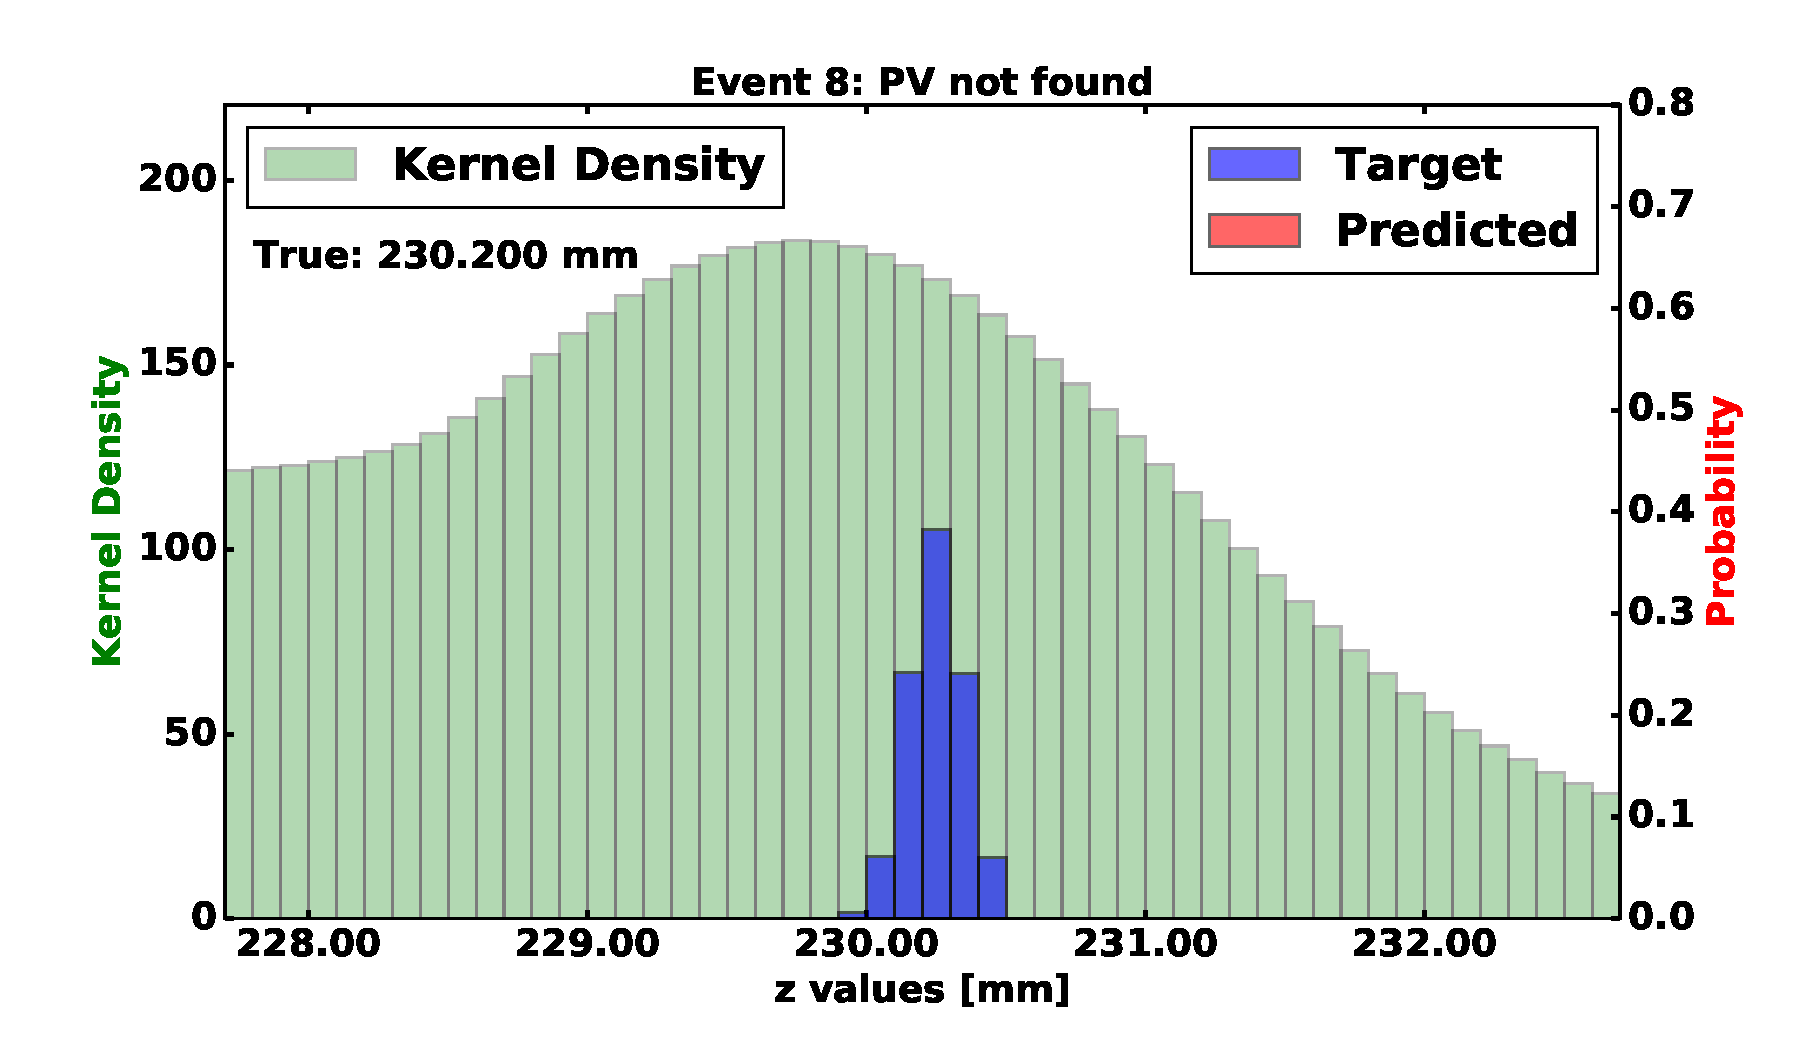
\includegraphics[width=1\textwidth,height=0.45\textwidth, trim=18 0 18 0]{images/120000_3layer_53.pdf}

            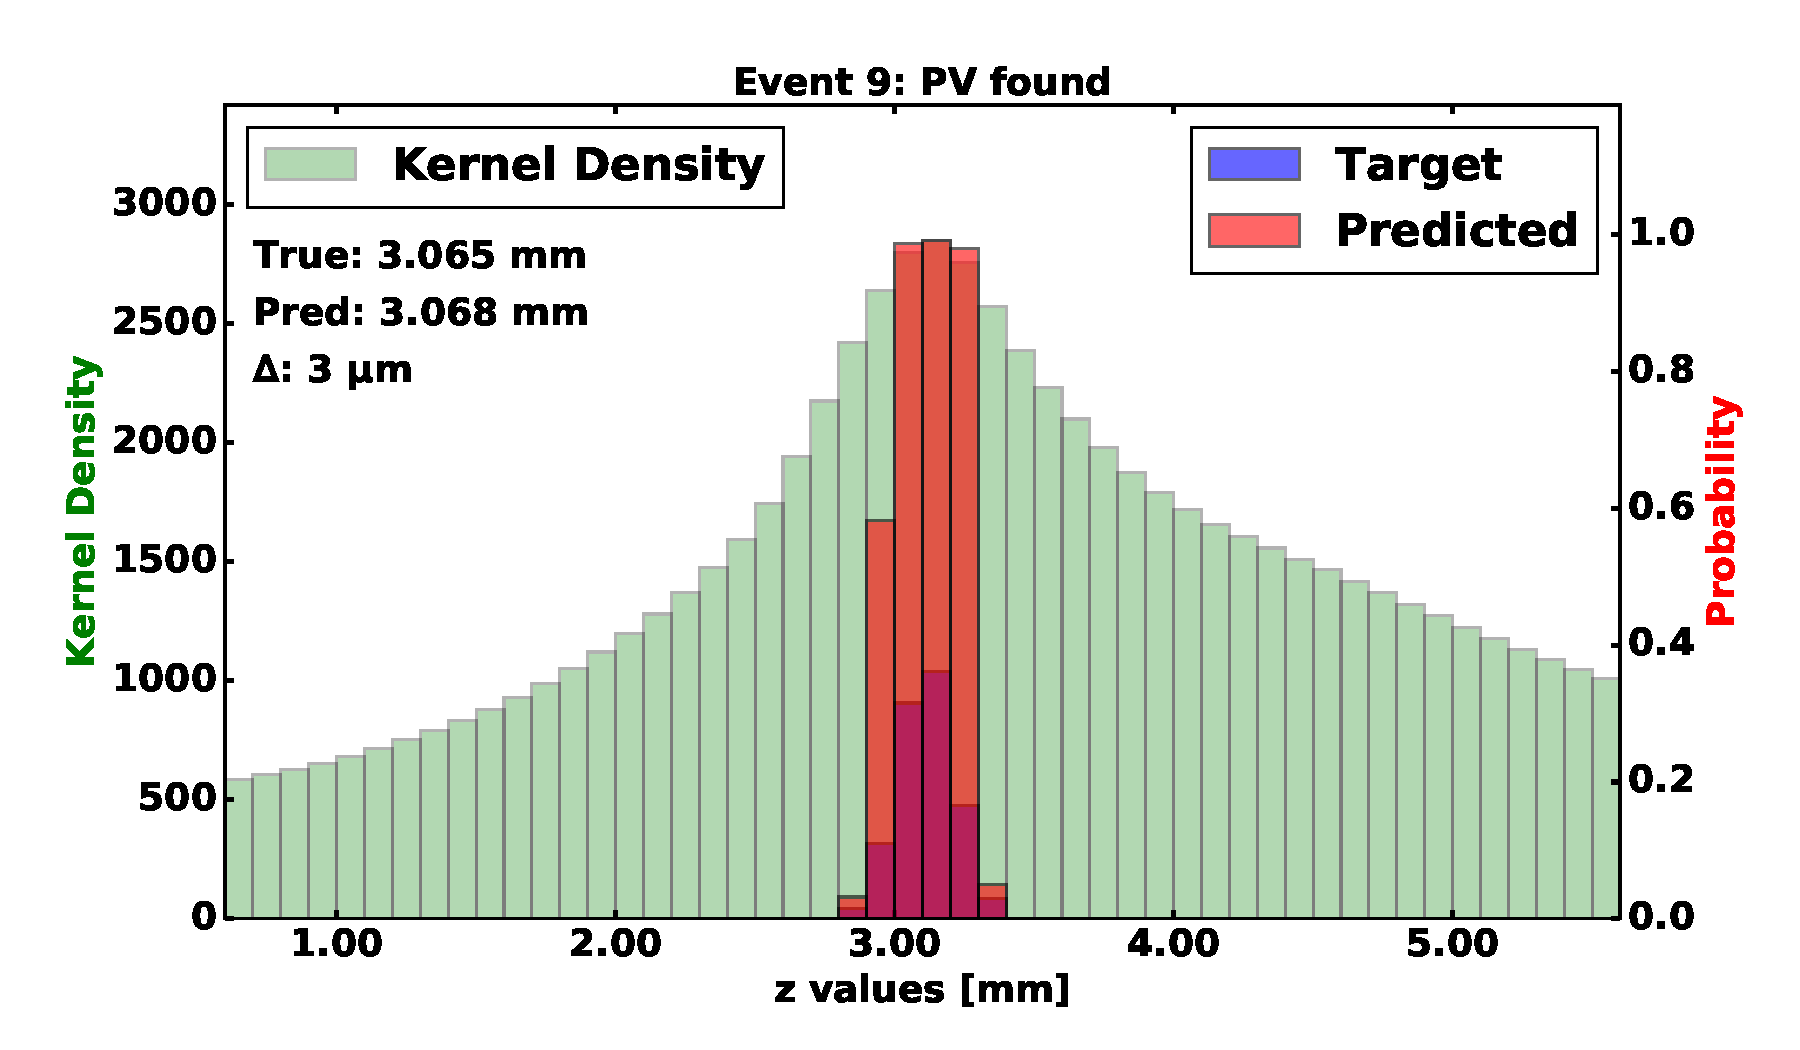
\includegraphics[width=1\textwidth, height=0.45\textwidth,trim=18 0 18 0]{images/120000_3layer_54.pdf}

        \end{center}
    \column{.5\textwidth}
        \begin{center}
           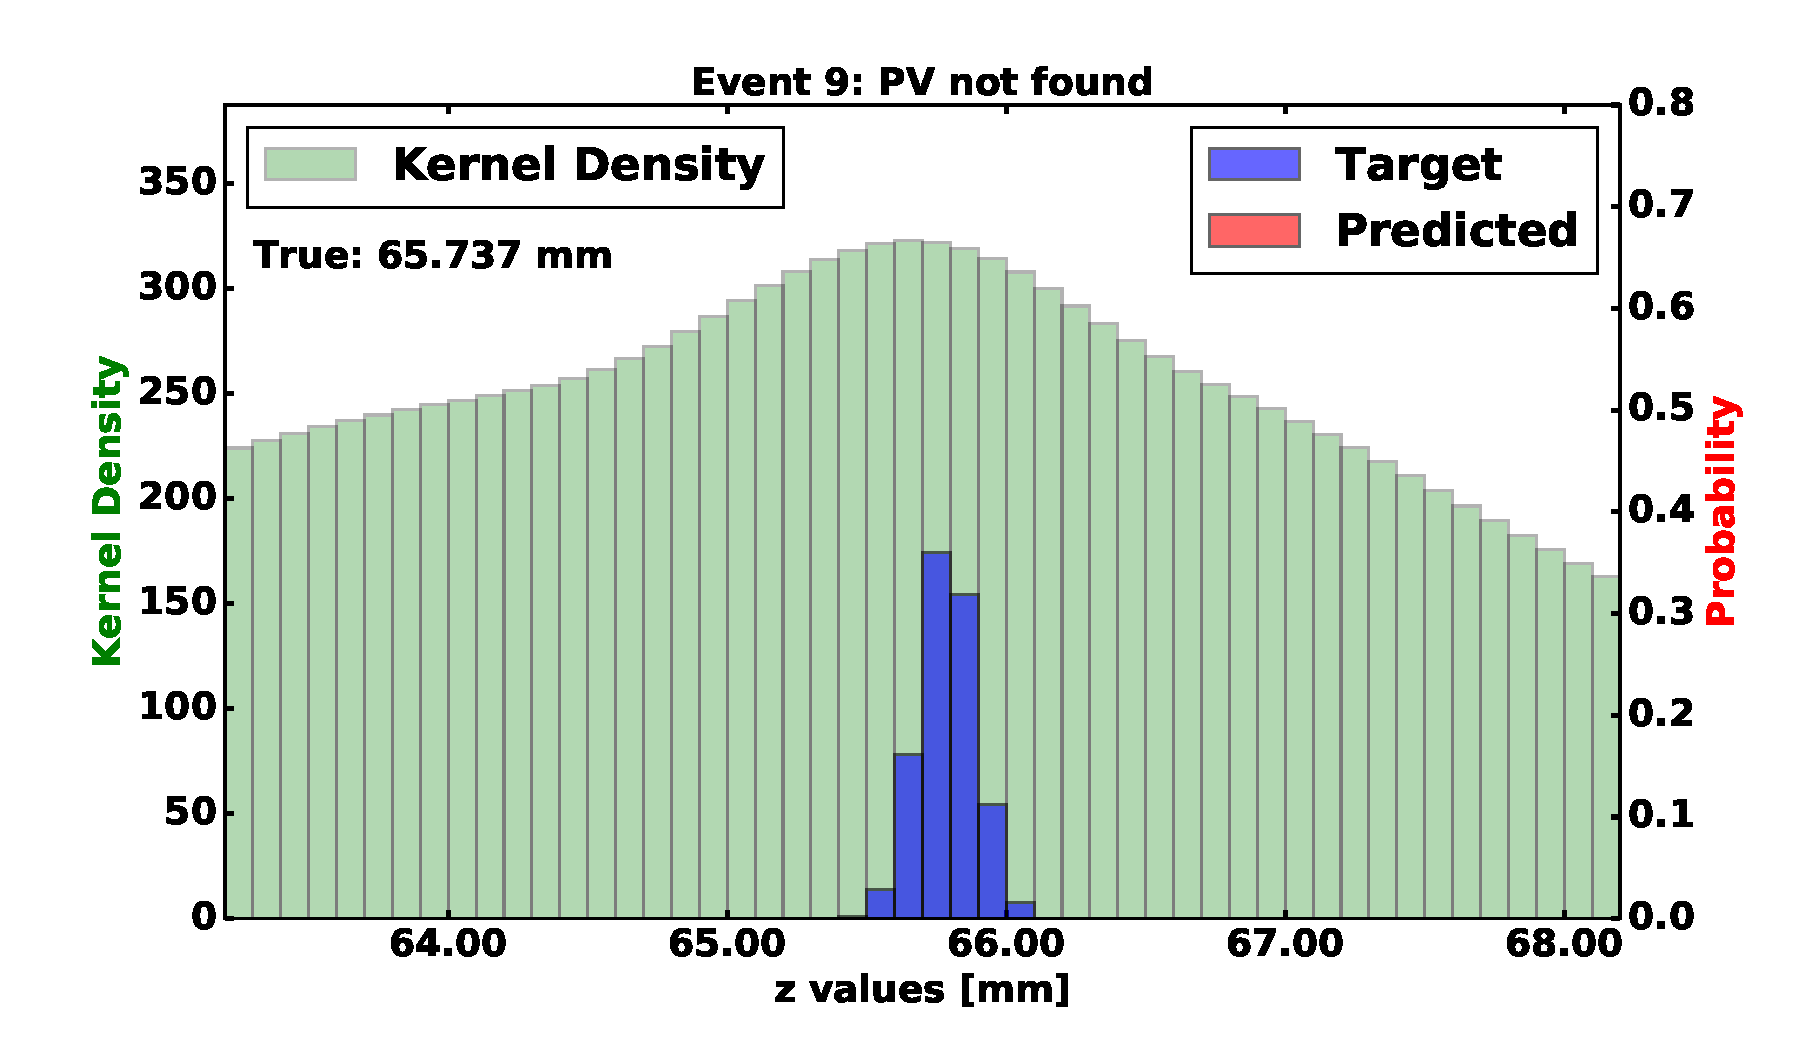
\includegraphics[width=1\textwidth, height=0.45\textwidth, trim=18 0 18 0]{images/120000_3layer_55.pdf}

           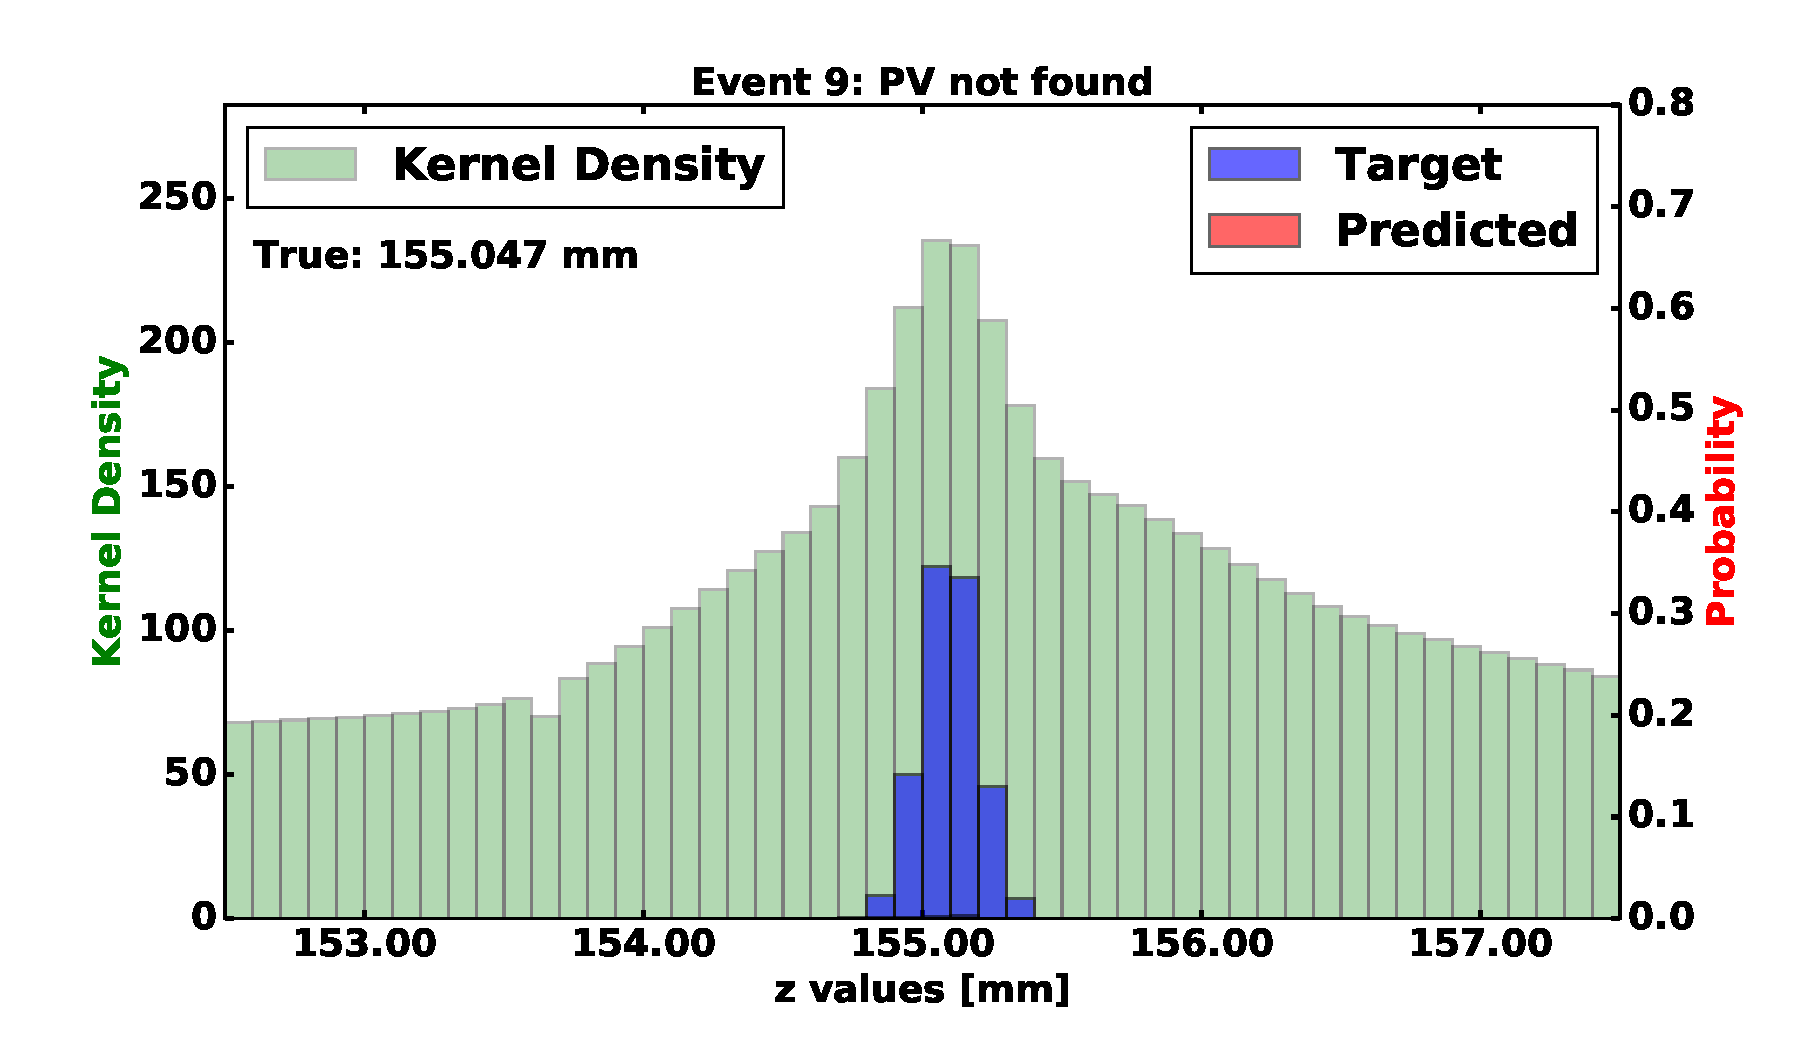
\includegraphics[width=1\textwidth, height=0.45\textwidth, trim=18 0 18 0]{images/120000_3layer_56.pdf}
       \end{center}
  \end{columns}
\end{frame}

\subsection{The VELO}
\begin{frame}{The VELO}
  \begin{columns}[c]
    \column{.6\textwidth}
    \begin{block}{Tracks}
      \begin{itemize}
          \item Originate from vertices (not shown)
          \item Hits originate from tracks
          \item We only know the true track in simulation
          \item Nearly straight, but tracks may scatter in material
      \end{itemize}
    \end{block}
    \begin{block}{The VELO}
      \begin{itemize}
          \item A set of 26 planes that detect tracks
          \item Tracks should hit one or more pixels per plane
          \item Sparse 3D dataset (41M pixels)
      \end{itemize}
    \end{block}
    \column{.4\textwidth}
    \centering
    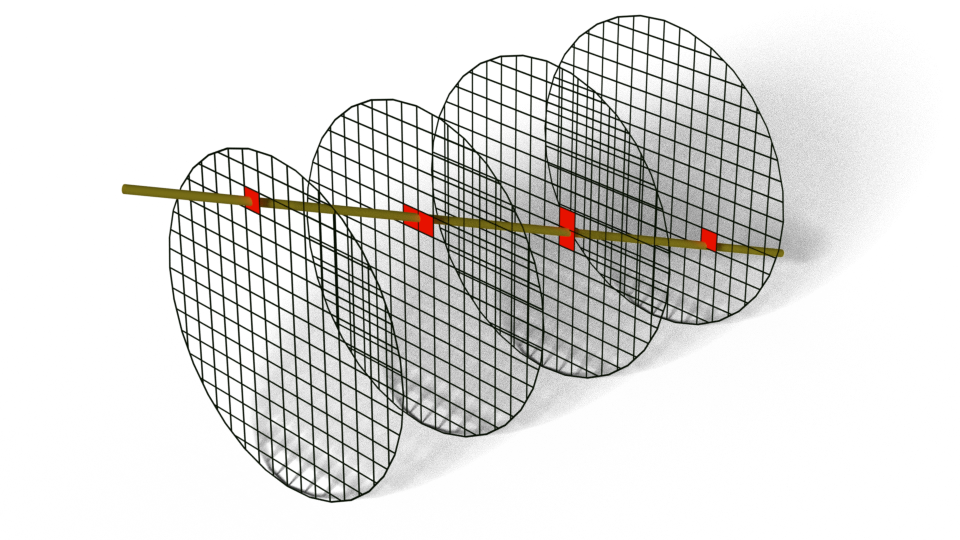
\includegraphics[width=\textwidth, trim=200 0 100 0]{images/Intersections.png}
  \end{columns}
\end{frame}
